\addbibresource{bib/os.bib}
\addbibresource{bib/wikipedia.bib}

\AtBeginPart{\frame{\partpage}}
\mode<beamer>{\AtBeginSection{\frame{\sectionpage}}}

% \includeonlylecture{intro}
% \includeonlylecture{proc}
% \includeonlylecture{ipc}
% \includeonlylecture{sched}
% \includeonlylecture{deadlock}
% \includeonlylecture{mm}
% \includeonlylecture{fs}
% \includeonlylecture{io}

\title{Operating Systems}
\author{Wang Xiaolin\\{\small \url{wx672ster+os@gmail.com}}}

\begin{document}

\mode<article>{  
  \subtitle{Lecture Handouts}
  \maketitle
  \tableofcontents
  \printbibliography[title={References}]}

\mode<beamer>{\frame{\titlepage}}

\begin{frame}<beamer>{Textbooks}
  \begin{refsection}
    \nocite{tanenbaum2008modern, silberschatz11essentials, bovet2005understanding,
      zhenggang2016, linuxkernelart13, yuyuan2009orange}%
    \printbibliography[heading=none]
  \end{refsection}
\end{frame}

\begin{frame}{Course Web Links}
  \begin{description}
  \item[Course web site:] \url{https://cs6.swfu.edu.cn/moodle}
  \item[Lecture slides:] \url{https://cs2.swfu.edu.cn/~wx672/lecture_notes/os/slides/}
  \item[Source code:] \url{https://cs2.swfu.edu.cn/~wx672/lecture_notes/os/src/}
  \item[Lab instructions] \url{https://cs2.swfu.edu.cn/~wx672/lecture_notes/os/lab.html}
  \item[Sample lab report:] \url{https://cs2.swfu.edu.cn/~wx672/lecture_notes/os/sample-report/}
  \end{description}
\end{frame}

\part{Introduction}

\lecture[intro]{intro}{intro}

\section{What's an Operating System}

\begin{frame}{What's an Operating System?}
  \begin{itemize}
  \item \emph{``Everything a vendor ships when you order an operating system''}
  \item It's the program that runs all the time
  \item It's a \alert{resource manager}
    \begin{itemize}
    \item[-] Each program gets time with the resource
    \item[-] Each program gets space on the resource
    \end{itemize}
  \item It's a \alert{control program}
    \begin{itemize}
    \item[-] Controls execution of programs to prevent errors and improper use of the
      computer
    \end{itemize}
  \item No universally accepted definition
  \end{itemize}
\end{frame}

\begin{frame}<beamer>{What's in the OS?}
  \begin{center}
    \includegraphics[height=.85\textheight]{kernel-block}
  \end{center}
\end{frame}

\begin{center}
  \includegraphics[width=\textwidth]{kernel-block}
\end{center}

\begin{frame}{Abstractions}{To hide the complexity of the actual implementations}
  \begin{center}
    \mode<beamer>{ 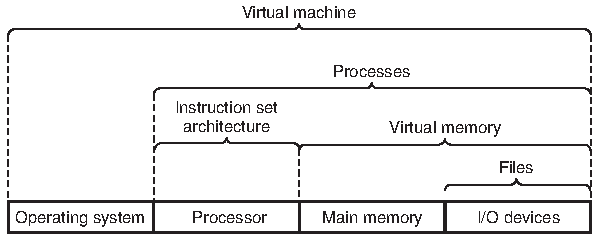
\includegraphics[width=\textwidth]{abstraction} }%
    \mode<article>{ 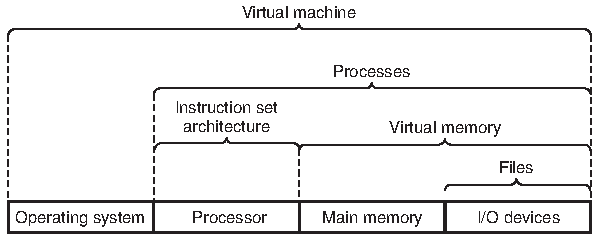
\includegraphics[width=.5\textwidth]{abstraction} }
  \end{center}
\end{frame}

See also: \citetitle[Sec.~1.9.2, \emph{The Importance of Abstractions in Computer
  Systems}]{Bryant2010computersystems}.

\begin{frame}{System Goals}
  \begin{block}{Convenient vs. Efficient}
    \begin{itemize}
    \item Convenient for the user --- for PCs
    \item Efficient --- for mainframes, multiusers
    \item UNIX
      \begin{itemize}
      \item[-] Started with keyboard + printer, none paid to convenience
      \item[-] Now, still concentrating on efficiency, with GUI support
      \end{itemize}
    \end{itemize}
  \end{block}
\end{frame}

\begin{frame}{History of Operating Systems}
  \begin{center}
    \mode<beamer>{ 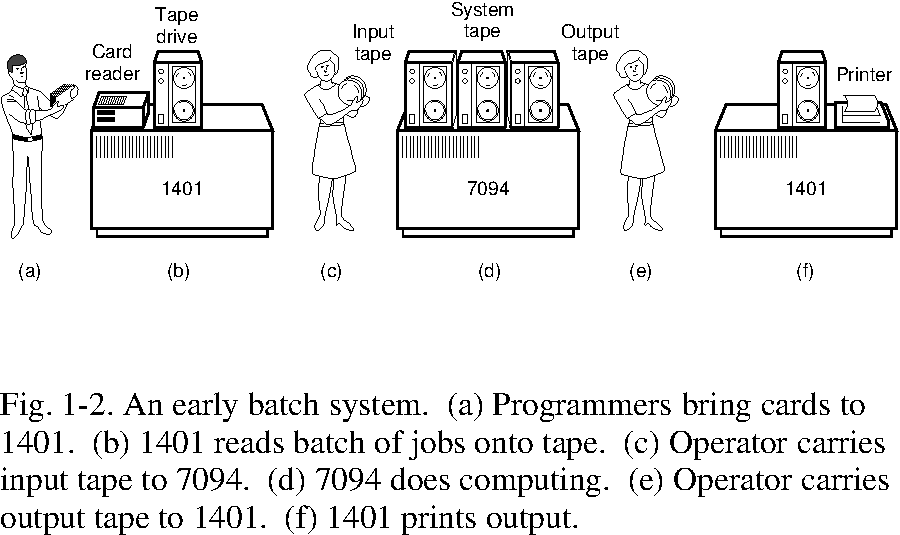
\includegraphics[width=\textwidth]{mos-figs-1-2} }%
    \mode<article>{ 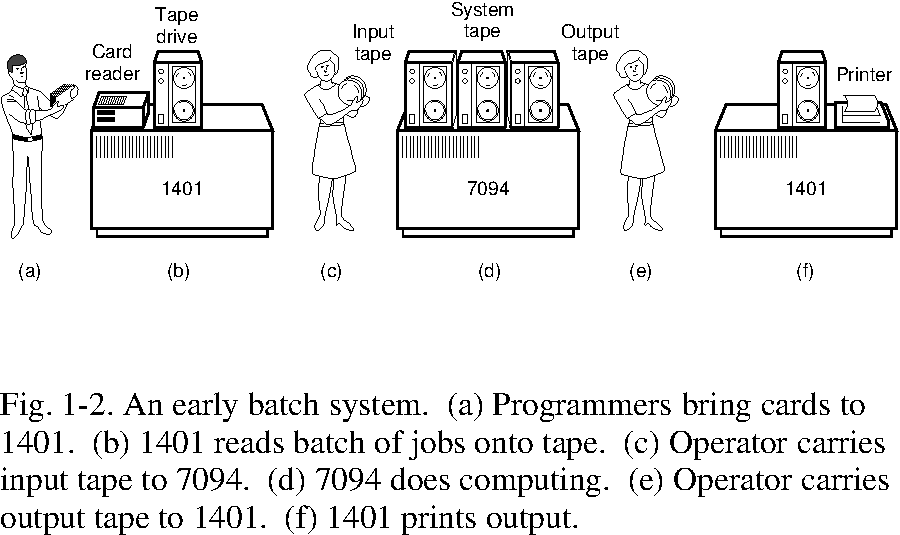
\includegraphics[width=.7\textwidth]{mos-figs-1-2} }
  \end{center}
\end{frame}

\begin{frame}
  \begin{description}
  \item[1945 - 1955] First generation 
    \begin{itemize}
    \item[-] vacuum tubes, plug boards
    \end{itemize}
  \item[1955 - 1965] Second generation 
    \begin{itemize}
    \item[-] transistors, batch systems
    \end{itemize}
  \item[1965 - 1980] Third generation 
    \begin{itemize}
    \item[-] ICs and multiprogramming
    \end{itemize}
  \item[1980 - present] Fourth generation 
    \begin{itemize}
    \item[-] personal computers
    \end{itemize}
  \end{description}
\end{frame}

\begin{frame}
  \begin{block}{Multi-programming is the first instance where the OS must make decisions
      for the users}
    \begin{minipage}{.65\linewidth}
      \begin{description}
      \item[Job scheduling] --- decides which job should be loaded into the memory.
      \item[Memory management] --- because several programs in memory at the same time
      \item[CPU scheduling] --- choose one job among all the jobs are ready to run
      \item[Process management] --- make sure processes don't offend each other
      \end{description}
    \end{minipage}\quad
    \begin{minipage}{.3\linewidth}
      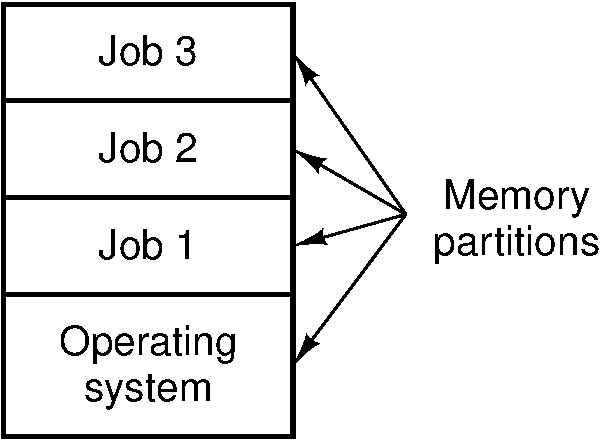
\includegraphics[width=\textwidth]{mos-figs-1-4}
    \end{minipage}
  \end{block}
\end{frame}

\begin{frame}{The Operating System Zoo}
    \begin{itemize}
    \item {\huge Mainframe OS}
    \item {\LARGE Server OS}
    \item {\Large Multiprocessor OS}
    \item {\large Personal computer OS}
    \item Real-time OS
    \item {\small Embedded OS}
    \item {\scriptsize Smart card OS}
    \end{itemize}
\end{frame}

\section{OS Services}

\begin{frame}{OS Services}{Like a government}
  \begin{block}{Helping the users:}
    \begin{multicols}{2}
      \begin{itemize}
      \item User interface
      \item Program execution
      \item I/O operation
      \item File system manipulation
      \item Communication
      \item Error detection
      \end{itemize}
    \end{multicols}
  \end{block}
  \begin{block}{Keeping the system efficient:}
  \begin{itemize}
  \item Resource allocation
  \item Accounting
  \item Protection and security
  \end{itemize}
  \end{block}
\end{frame}

\begin{frame}{A Computer System}
  \begin{center}
    \mode<beamer>{ 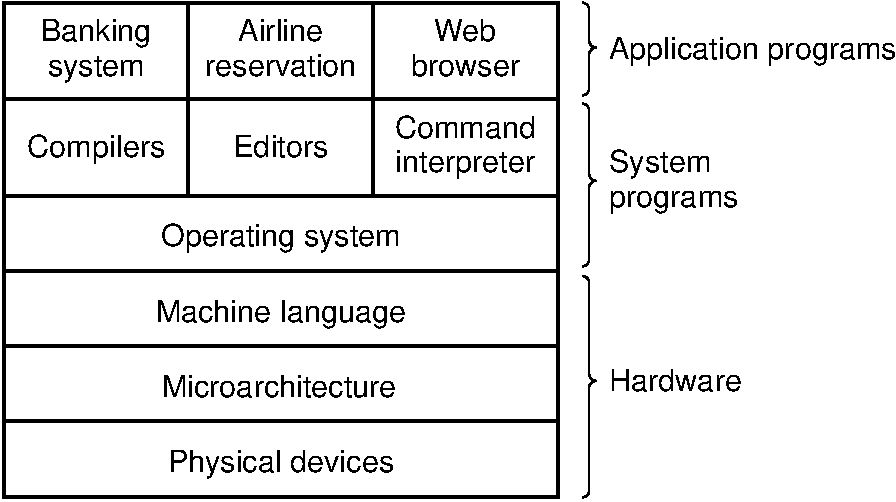
\includegraphics[width=\textwidth]{mos-figs-1-1} }%
    \mode<article>{ 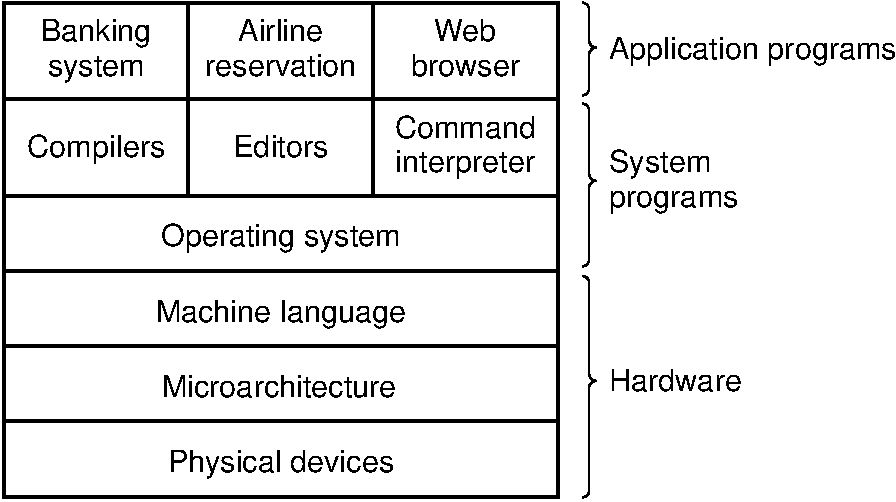
\includegraphics[width=.5\textwidth]{mos-figs-1-1} }
  \end{center}
\end{frame}

\section{Hardware}
\label{sec:cpu}

% \begin{frame}<beamer>{Outline}
%   \tableofcontents[currentsection,currentsubsection]
% \end{frame}

\begin{frame}{CPU Working Cycle}
  \begin{center}
    \mode<beamer>{ 
\includegraphics[width=.6\textwidth]{mos-figs-1-6} }%
    \mode<article>{ 
\includegraphics[width=.3\textwidth]{mos-figs-1-6} }
  \end{center}
  \begin{enumerate}
  \item Fetch the first instruction from memory
  \item Decode it to determine its type and operands
  \item execute it
  \end{enumerate}
  \begin{block}{Special CPU Registers}
    \begin{description}
    \item[Program counter (PC):] keeps the memory address of the next instruction to
      be fetched
    \item[Stack pointer (SP):] {\symbola ☛} the top of the current stack in memory
    \item[Program status (PS):] holds
      \begin{itemize}
      \item[-] condition code bits
      \item[-] processor state
      \end{itemize}
    \end{description}
  \end{block}
\end{frame}

\begin{frame}{System Bus}
  \begin{center}
    \mode<beamer>{ 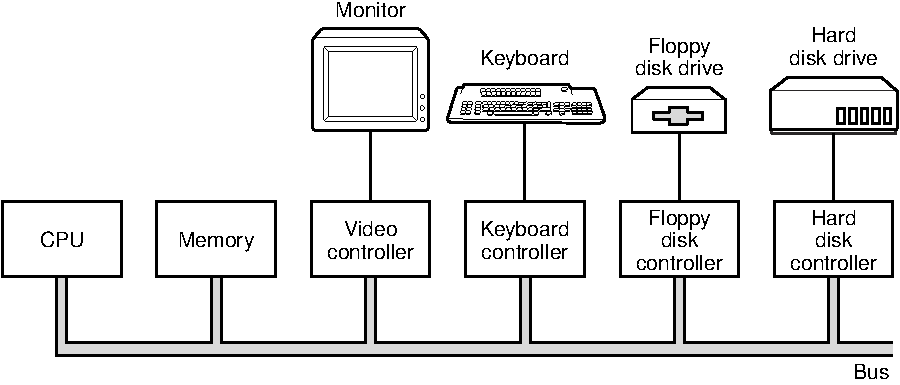
\includegraphics[width=\textwidth]{mos-figs-1-5} }%
    \mode<article>{ 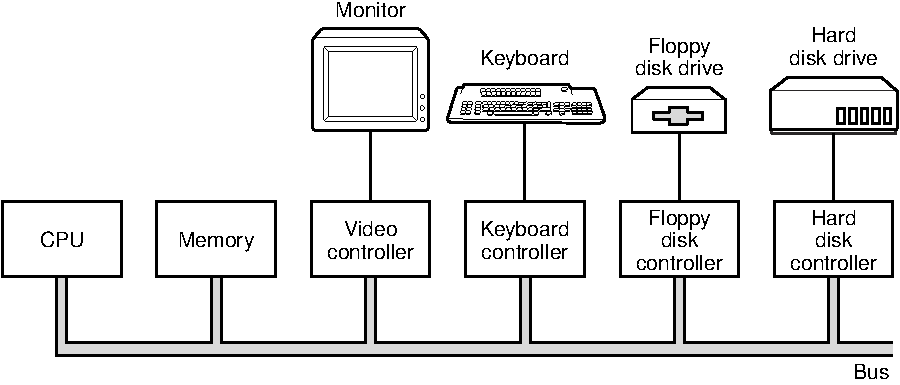
\includegraphics[width=.6\textwidth]{mos-figs-1-5} }
  \end{center}
  \begin{description}
  \item[Address Bus:] specifies the memory locations (addresses) for the
    data transfers
  \item[Data Bus:] holds the data transfered. Bidirectional
  \item[Control Bus:] contains various lines used to route timing and
    control signals throughout the system
  \end{description}
\end{frame}

\begin{frame}{Controllers and Peripherals}
  \begin{itemize}
  \item Peripherals are real devices controlled by controller chips
  \item Controllers are processors like the CPU itself, have control registers
  \item Device driver writes to the registers, thus control it
  \item Controllers are connected to the CPU and to each other by a variety of buses
  \end{itemize}
\end{frame}

\begin{frame}
  \begin{center}
    \mode<beamer>{ 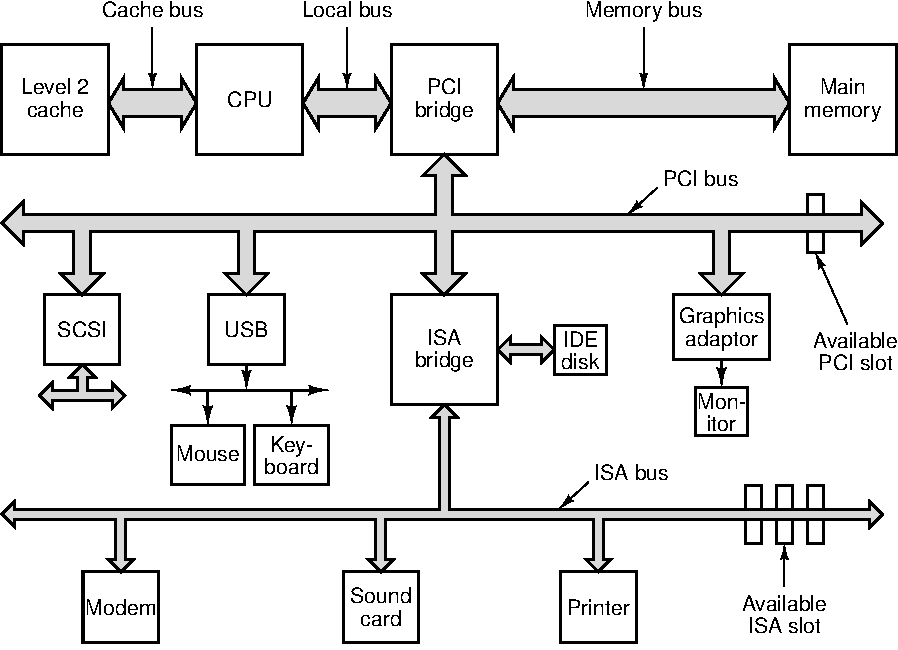
\includegraphics[width=\textwidth]{mos-figs-1-11} }%
    \mode<article>{ 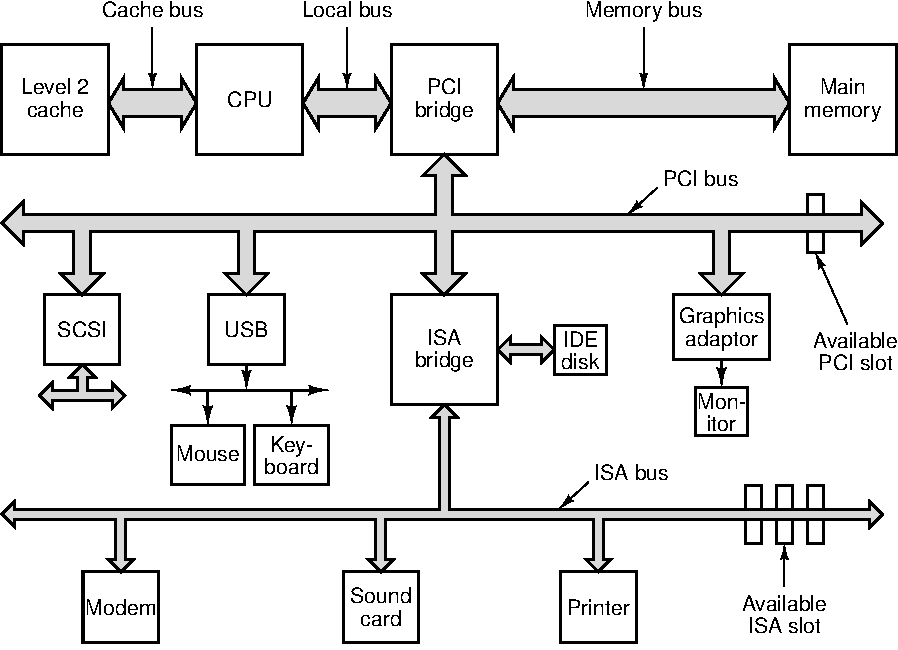
\includegraphics[width=.6\textwidth]{mos-figs-1-11} }
  \end{center}
\end{frame}

\begin{frame}{Motherboard Chipsets}
  \begin{center}
    \mode<beamer>{ 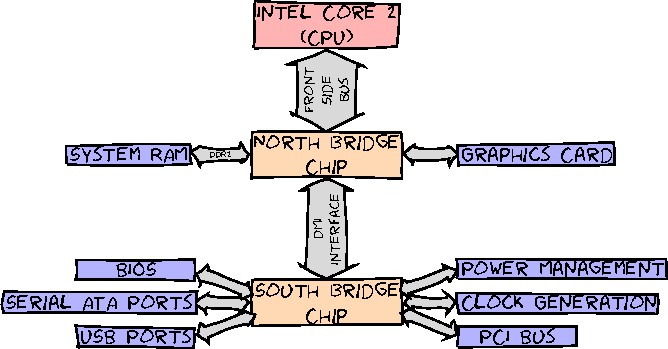
\includegraphics[width=\textwidth]{chipsets} }
    \mode<article>{ \includegraphics[width=.5\textwidth]{chipsets-bw} }
  \end{center}
\end{frame}

See also:
\href{http://duartes.org/gustavo/blog/post/motherboard-chipsets-memory-map}{\emph{Motherboard
    Chipsets And The Memory Map}}
\footnote{\url{http://duartes.org/gustavo/blog/post/motherboard-chipsets-memory-map}}.

\begin{frame}
  \begin{itemize}
  \item The CPU doesn't know what it's connected to
    \begin{itemize}
    \item[-] CPU test bench?\quad{}network router?\quad{}toaster?\quad{}brain implant?
    \end{itemize}
  \item The CPU talks to the outside world through its pins
    \begin{itemize}
    \item[-] some pins to transmit the physical memory address
    \item[-] other pins to transmit the values
    \end{itemize}
  \item The CPU's gateway to the world is the \alert{front-side bus}
  \end{itemize}
  \begin{block}{Intel Core 2 QX6600}
    \begin{itemize}
    \item 33 pins to transmit the physical memory address
      \begin{itemize}
      \item[-] so there are $2^{33}$ choices of memory locations
      \end{itemize}
    \item 64 pins to send or receive data
      \begin{itemize}
      \item[-] so data path is 64-bit wide, or 8-byte chunks
      \end{itemize}
    \end{itemize}
    This allows the CPU to physically address 64GB of memory ($2^{33}\times{}8B$)    
  \end{block}
\end{frame}

See also:
\href{http://download.intel.com/design/processor/datashts/31559205.pdf}{\emph{Datasheet
    for Intel Core 2 Quad-Core Q6000 Sequence}}
\footnote{\url{http://download.intel.com/design/processor/datashts/31559205.pdf}}.

\begin{frame}[plain]
  \begin{minipage}{.65\linewidth}
    \begin{block}{Some physical memory addresses are mapped away!}
      \begin{itemize}
      \item only the addresses, not the spaces
      \item Memory holes
        \begin{itemize}
        \item[-] $640KB \sim 1MB$
        \item[-] \texttt{/proc/iomem}
        \end{itemize}
      \end{itemize}
    \end{block}
    \begin{block}{Memory-mapped I/O}
      \begin{itemize}
      \item BIOS ROM
      \item video cards
      \item PCI cards
      \item \ldots
      \end{itemize}
      This is why 32-bit OSes have problems using 4 gigs of RAM.
    \end{block}
  \end{minipage}\quad
  \begin{minipage}{.3\linewidth}
    \tikz[baseline,overlay]{
      \node [xshift=1.5cm,yshift=-1cm] at (0,0) {
        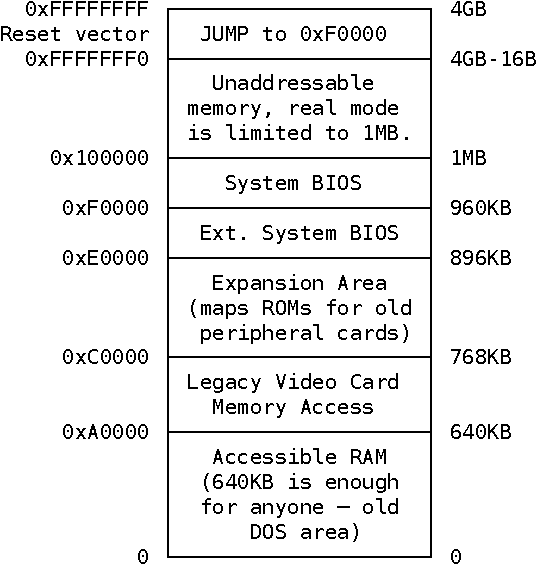
\includegraphics[scale=0.62]{boot-mem}}}
  \end{minipage}
  % \begin{center}
  %   What if you don't have 4G RAM?
  % \end{center}
\end{frame}

\begin{frame}
  \begin{block}{the northbridge}
    \begin{enumerate}
    \item receives a physical memory request
    \item decides where to route it
      \begin{itemize}
      \item[-] to RAM? to video card? to \ldots{}?
      \item[-] decision made via the \alert{memory address map}
      \end{itemize}
    \end{enumerate}
  \end{block}
\end{frame}

\begin{itemize}
\item When is the memory address map built? \texttt{setup()}.
\end{itemize}

\section{Bootstrapping}
\label{sec:bootstrapping}

\begin{frame}{Bootstrapping}
  \begin{block}{Can you pull yourself up by your own bootstraps?}
    \begin{itemize}
    \item[] A computer cannot run without first loading software but must be running
      before any software can be loaded.
    \end{itemize}
  \end{block}
  \begin{center}
    \mode<beamer>{ 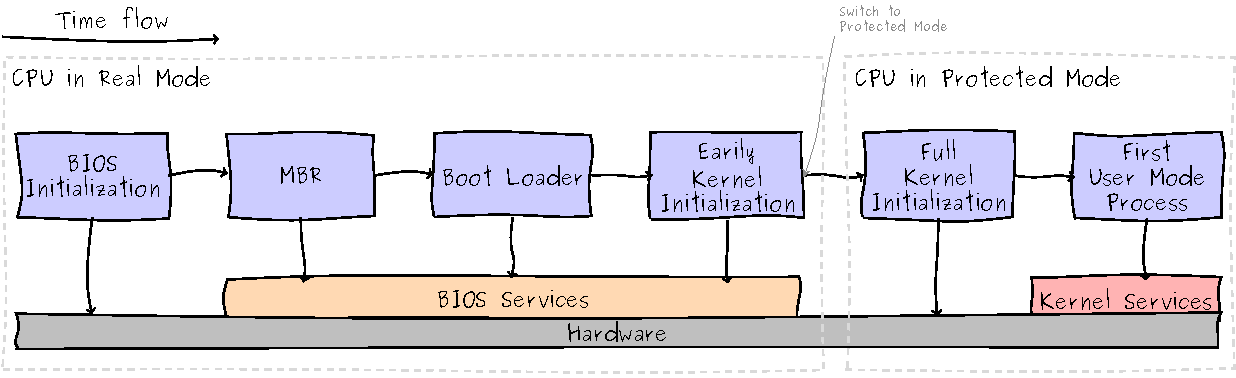
\includegraphics[width=\textwidth]{boot}}%
    \mode<article>{ \includegraphics[width=.7\textwidth]{boot-bw}}
  \end{center}
\end{frame}

\begin{frame}{Intel x86 Bootstrapping}
  \begin{enumerate}
  \item BIOS (\texttt{0xfffffff0})\\
    \begin{small}
      {\Symbol{➠}} POST\quad
      {\Symbol{➠}} HW init\quad
      {\Symbol{➠}} Find a boot device (FD,CD,HD\ldots{})\quad
      {\Symbol{➠}} Copy \alert{sector zero (MBR)} to RAM (\texttt{0x00007c00})
    \end{small}
  \item MBR -- the first 512 bytes, contains
    \begin{itemize}
    \item Small code ($< 446\,Bytes$), e.g. GRUB stage 1, for loading GRUB stage 2
    \item the primary partition table ($16\times{}4=64\,Bytes$)
    \item its job is to load the second-stage boot loader.
    \end{itemize}
  \item GRUB stage 2 --- load the OS kernel into RAM
  \item {\linux} startup
  \item init --- the first user-space program
  \end{enumerate}
  \begin{center}
    \mode<beamer>{ \includegraphics[width=.8\textwidth]{mbr}}%
    \mode<article>{ \includegraphics[width=.5\textwidth]{mbr}}
  \end{center}
  \begin{itemize}
  \item[\$] \texttt{sudo hd -n512 /dev/sda}
  \end{itemize}
\end{frame}

\section{Interrupt}
\label{sec:interrupt}

% \begin{frame}<beamer>{Outline}
%   \tableofcontents[currentsection,currentsubsection]
% \end{frame}

\begin{frame}{Why Interrupt?}
  \begin{block}{While a process is reading a disk file, can we do...}
    \begin{center}
      \mode<beamer>{ \includegraphics[width=.6\textwidth]{interrupt}}%
      \mode<article>{ 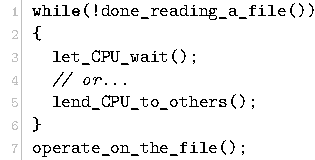
\includegraphics[width=.3\textwidth]{interrupt-bw}}
    \end{center}
  \end{block}
\end{frame}

\begin{frame}{Modern OS are Interrupt Driven}
  \begin{description}
  \item[HW INT] by sending a signal to CPU
  \item[SW INT] by executing a \alert{system call}
  \item[Trap (exception)] is a software-generated INT coursed by an error or by a
    specific request from an user program
  \item[Interrupt vector] is an array of pointers {\pright} the memory addresses
    of \alert{interrupt handlers}. This array is indexed by a unique device number
    \begin{itemize}
    \item[\$] \texttt{less /proc/devices}
    \item[\$] \texttt{less /proc/interrupts}
    \end{itemize}
  \end{description}
\end{frame}

\begin{frame}{Programmable Interrupt Controllers}
  \begin{center}
    \mode<beamer>{ 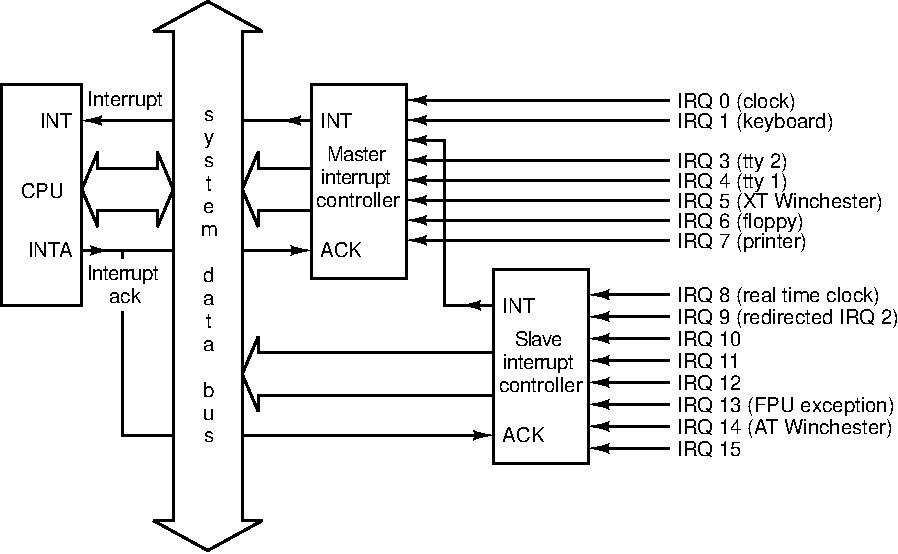
\includegraphics[width=\textwidth]{int-osdi-34}}%
    \mode<article>{ 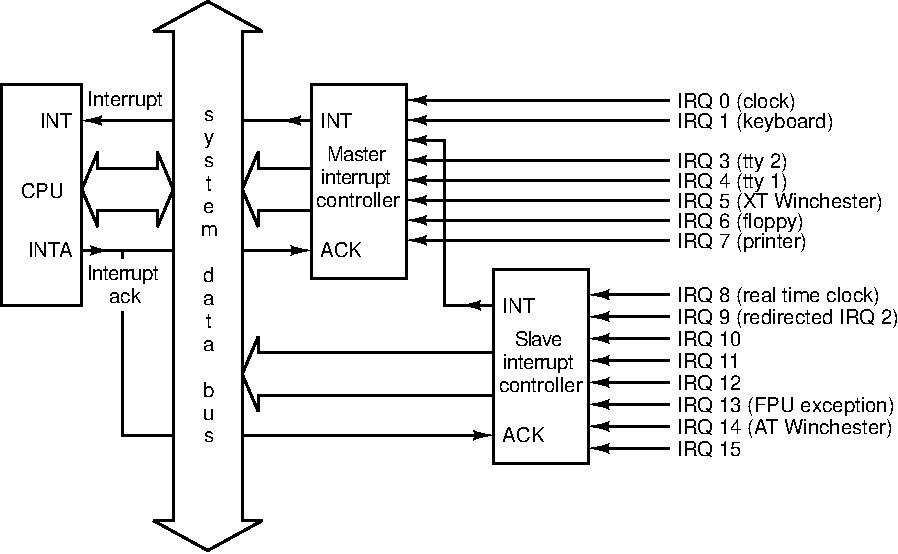
\includegraphics[width=.5\textwidth]{int-osdi-34}}
  \end{center}
\end{frame}

\begin{frame}{Interrupt Processing}
  % 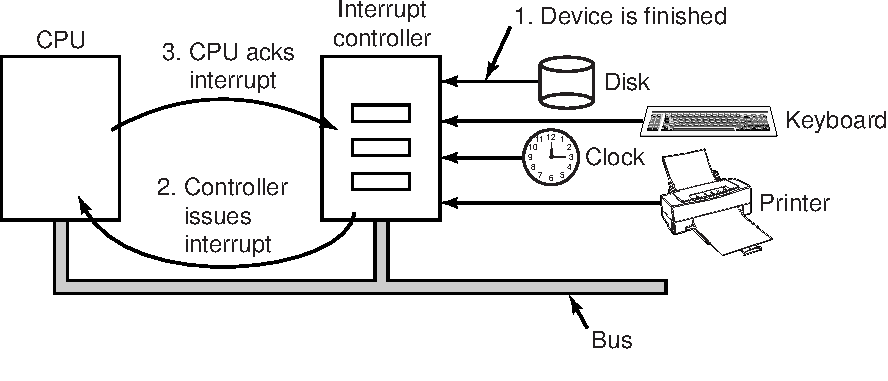
\includegraphics[width=.9\textwidth]{int-mos-figs-5-6}\\
  \begin{center}
    \mode<beamer>{ 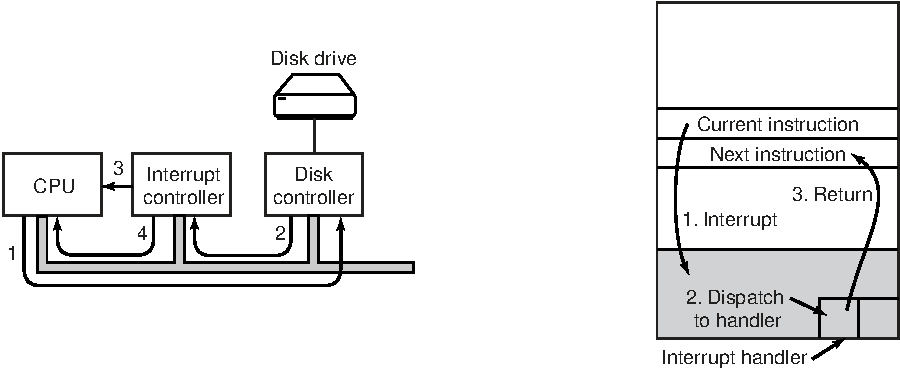
\includegraphics[width=\textwidth]{mos-figs-1-10} }%
    \mode<article>{ 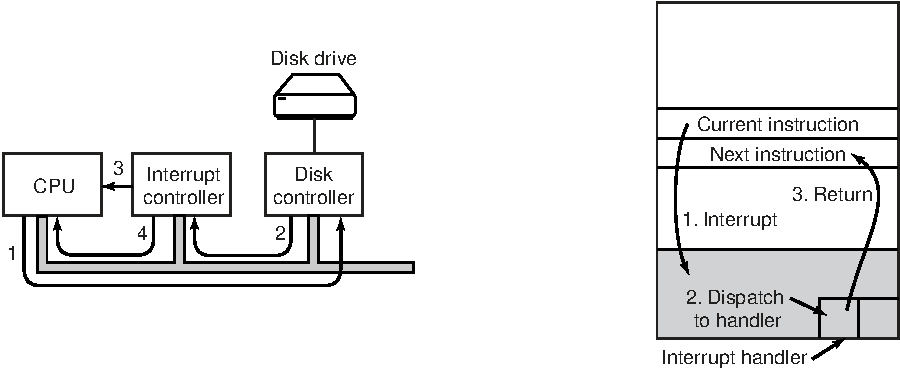
\includegraphics[width=.7\textwidth]{mos-figs-1-10} }
  \end{center}
\end{frame}

Detailed explanation: in \citetitle[Sec.~1.3.5, \emph{I/O Devices}]{tanenbaum2008modern}.

\begin{frame}{Interrupt Timeline}
  \begin{center}
    \mode<beamer>{ 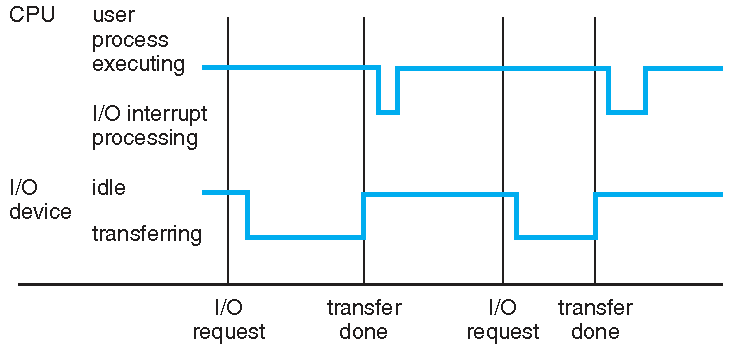
\includegraphics[width=\textwidth]{ir-timeline} }%
    \mode<article>{ 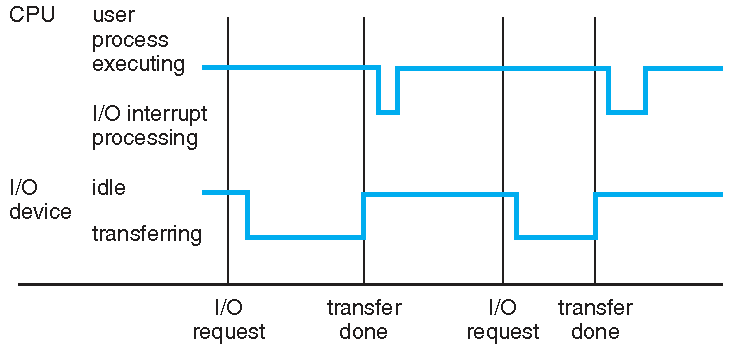
\includegraphics[width=.5\textwidth]{ir-timeline} }
  \end{center}
\end{frame}

\section{System Calls}
\label{sec:system-calls}

% \begin{frame}<beamer>{Outline}
%   \tableofcontents[currentsection,currentsubsection]
% \end{frame}

\begin{frame}{System Calls}
  \begin{block}{A System Call}
  \begin{itemize}
  \item is how a program requests a service from an OS kernel
  \item provides the interface between a process and the OS
  \end{itemize}
  \end{block}
\end{frame}

\begin{frame}
  \begin{center}
    \mode<beamer>{
      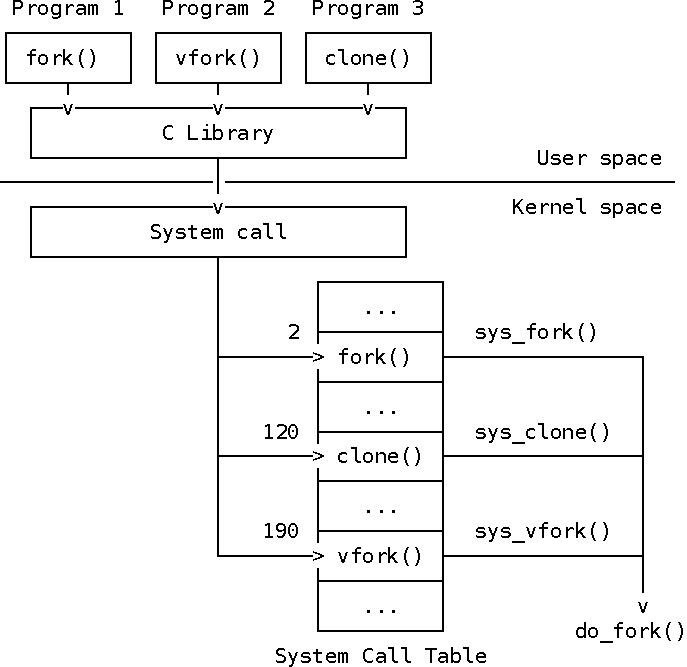
\includegraphics[height=\textheight]{syscall}
    }
    \mode<article>{
      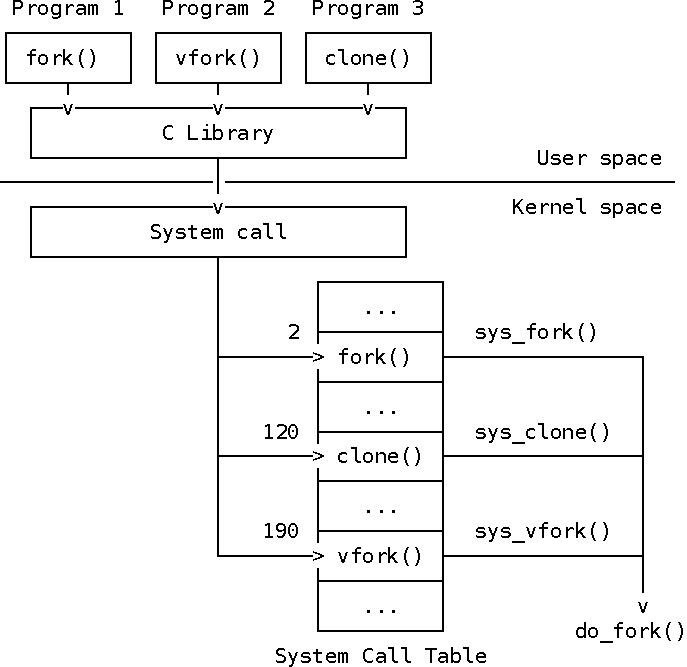
\includegraphics[width=.5\textwidth]{syscall}
    }
  \end{center}
\end{frame}

\begin{frame}%{System Calls}
  \begin{center}
    \mode<beamer>{
      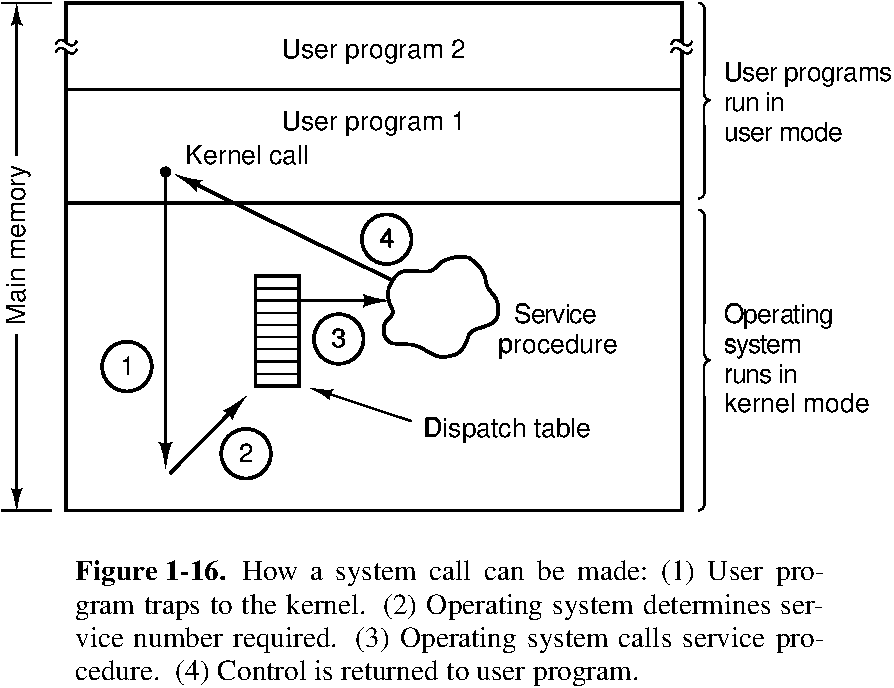
\includegraphics[width=\textwidth]{osdi2-1-18}
    }
    \mode<article>{
      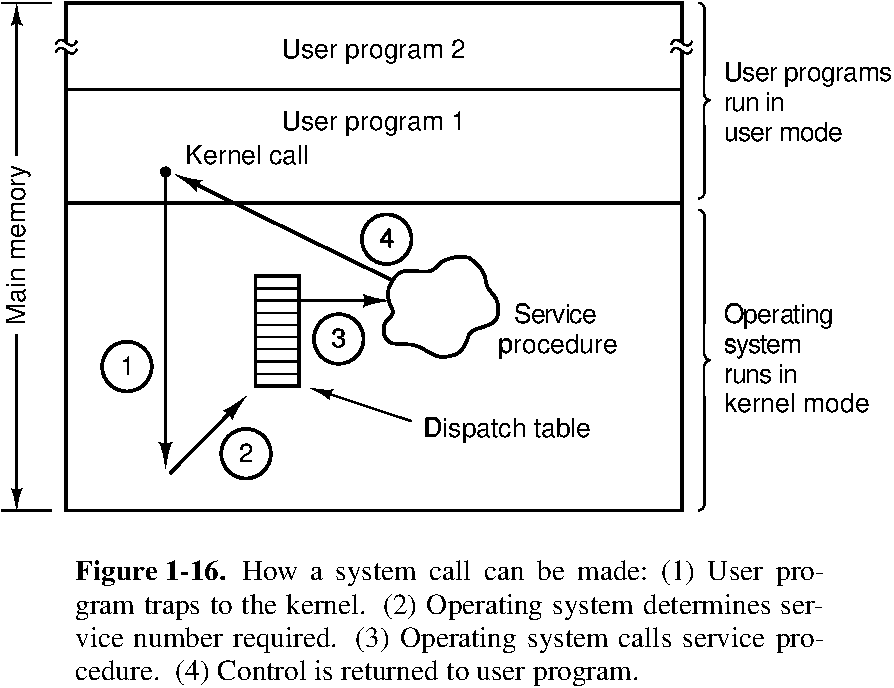
\includegraphics[width=.7\textwidth]{osdi2-1-18}
    }
  \end{center}
\end{frame}

% \begin{frame} {System Calls}
%   \includegraphics[width=\textwidth]{syscall1}
% \end{frame}

\begin{frame}
  \begin{block}{The 11 steps in making the system call \texttt{read(fd,buffer,nbytes)}}
    \begin{center}
      \mode<beamer>{
        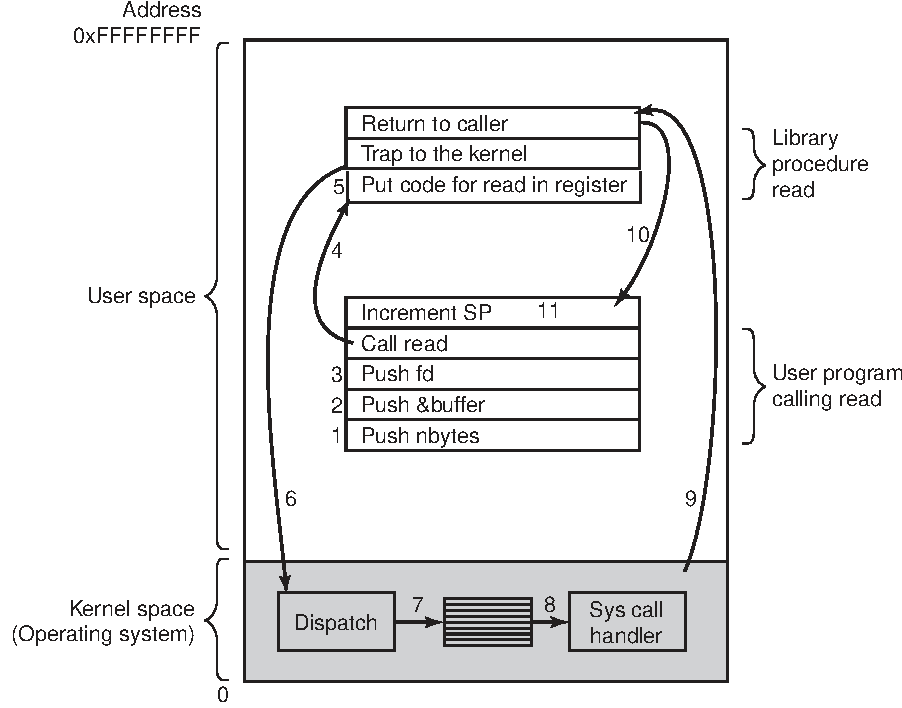
\includegraphics[width=.85\textwidth]{mos-figs-1-18}
      }
      \mode<article>{
        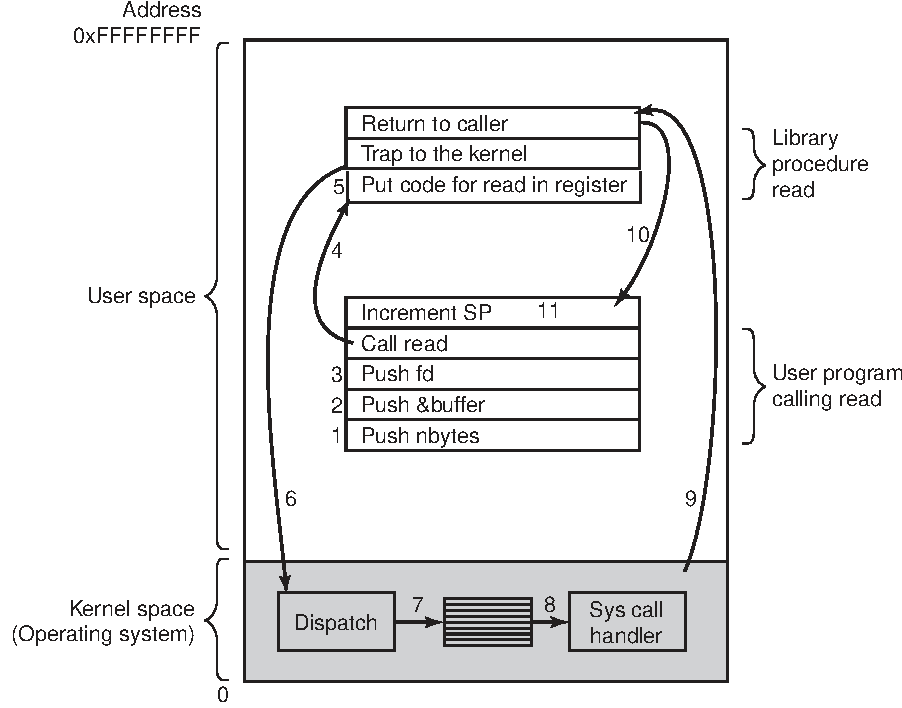
\includegraphics[width=.7\textwidth]{mos-figs-1-18}
      }
    \end{center}
  \end{block}
\end{frame}

\begin{frame}{Example}{Linux INT80h}
  \begin{description}
  \item[Interrupt Vector Table:] The very first 1KiB of x86 memory. 
    \begin{itemize} 
    \item 256 entries $\times$ 4B = 1KiB
    \item Each entry is a complete memory address (segment:offset)
    \item It's populated by Linux and BIOS
    \item Slot 80h: address of the kernel services dispatcher ({\pright} sys-call table)
    \end{itemize}
  \end{description}
\end{frame}

\begin{frame}[fragile]{Example}
\begin{nasmcode}
Msg: db "Hello, world"
MsgLen: equ $-Msg

mov eax,4      ; Specify sys_write syscall
mov ebx,1      ; Specify File Descriptor 1 (STDOUT)
mov ecx,Msg    ; Pass offset of the message
mov edx,MsgLen ; Pass the length of the message
int 80H        ; Make syscall to output the text to STDOUT
\end{nasmcode}
\end{frame}
%$
% \begin{frame} {System Calls}
%   \includegraphics[width=\textwidth]{syscall2}
% \end{frame}

\begin{frame}%{System Calls}
  \begin{center}
    \mode<beamer>{
      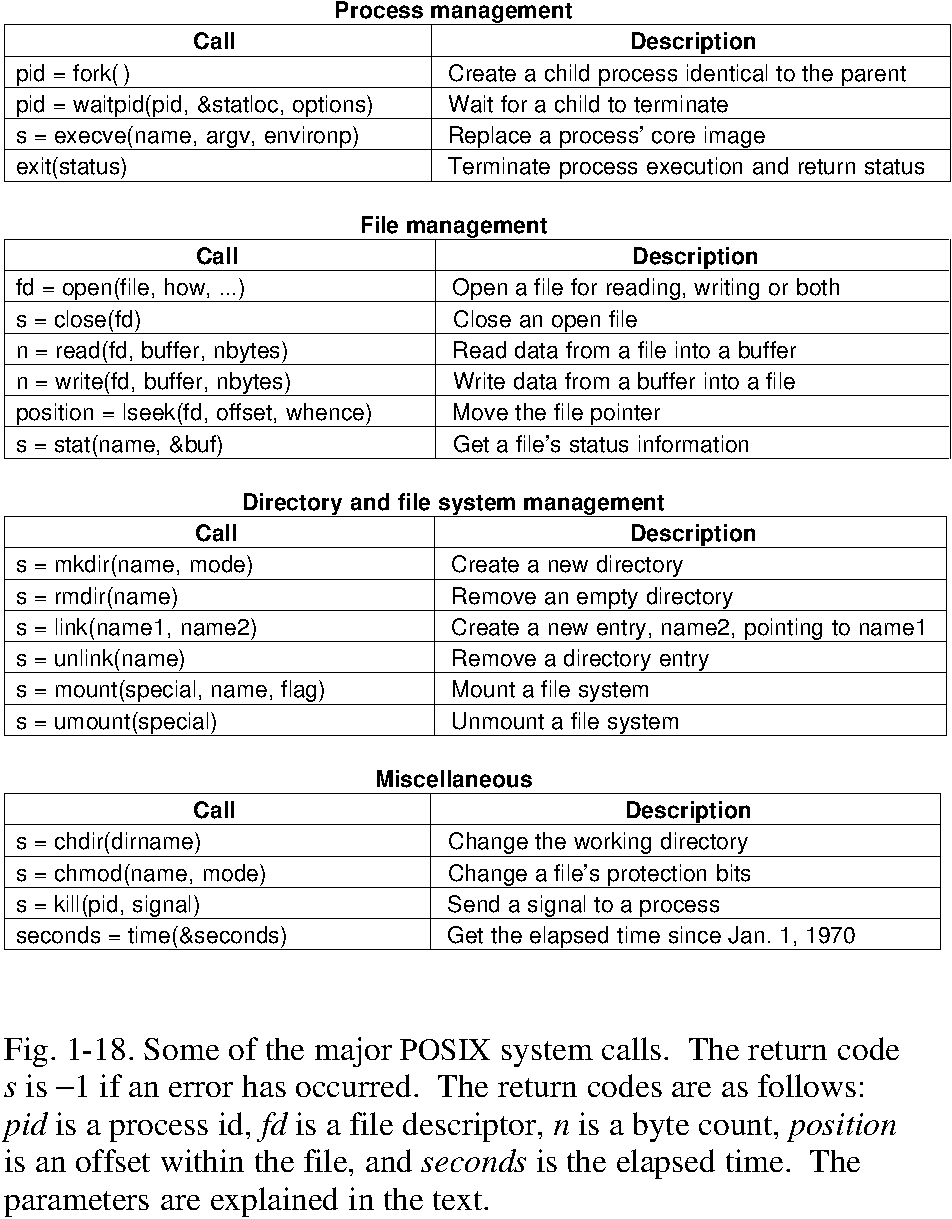
\includegraphics[width=.85\textwidth]{mos-figs-1-19}
    }
    \mode<article>{
      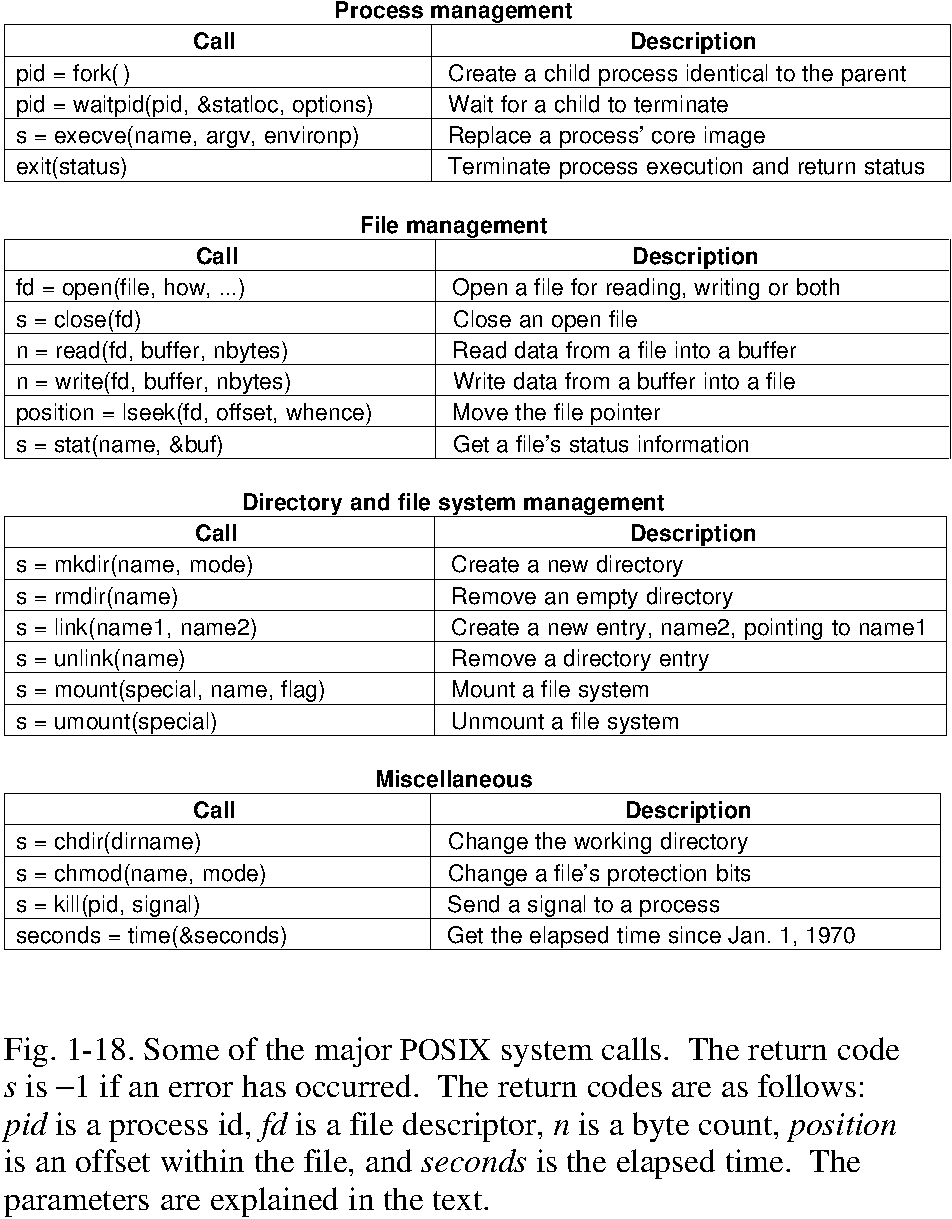
\includegraphics[width=.7\textwidth]{mos-figs-1-19}
    }
  \end{center}
\end{frame}

\begin{frame}{System Call Examples}
  \begin{block}{\texttt{fork()}}
    \begin{center}
      \mode<beamer>{
        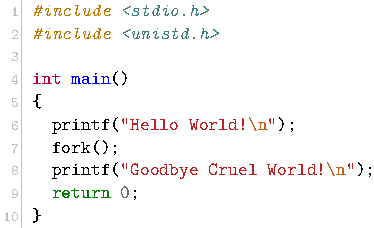
\includegraphics[width=.8\textwidth]{fork}
      } \mode<article>{
        \includegraphics[width=.4\textwidth]{fork-bw}
      }
    \end{center}
  \end{block}
  \begin{itemize}
  \item[\$] \texttt{man 2 fork}
  \end{itemize}
\end{frame}

\begin{frame}
  \begin{block}{\texttt{exec()}}
    \begin{center}
      \mode<beamer>{
        \includegraphics[width=\textwidth]{fork-exec}
      } \mode<article>{
        \includegraphics[width=.7\textwidth]{fork-exec-bw}
      }
    \end{center}
  \end{block}
  \begin{itemize}
  \item[\$] \texttt{man 3 exec}
  \end{itemize}
\end{frame}

Quoted from
\href{https://stackoverflow.com/questions/20823371/what-is-the-difference-between-the-functions-of-the-exec-family-of-system-calls}{
  stackoverflow: What is the difference between the functions of the \emph{exec} family of system calls}:

\begin{quote}
  There is no \emph{exec} system call --- this is usually used to refer to all the
  \emph{execXX} calls as a group. They all do essentially the same thing: loading a new
  program into the current process, and provide it with arguments and environment
  variables. The differences are in how the program is found, how the arguments are
  specified, and where the environment comes from.

  \begin{itemize}
  \item The calls with \emph{v} in the name take an array parameter to specify the
    \texttt{argv[]} array (\emph{vector}) of the new program.
  \item The calls with \emph{l} in the name take the arguments of the new program as a
    variable-length argument \emph{list} to the function itself.
  \item The calls with \emph{e} in the name take an extra argument to provide the
    \emph{environment} of the new program; otherwise, the program inherits the current
    process's environment.
  \item The calls with \emph{p} in the name search the \emph{PATH} environment variable to
    find the program if it doesn't have a directory in it (i.e. it doesn't contain a /
    character). Otherwise, the program name is always treated as a path to the executable.
  \end{itemize}
\end{quote}

\begin{frame}{Hardware INT vs. Software INT}
  \begin{center}
    \mode<beamer>{
      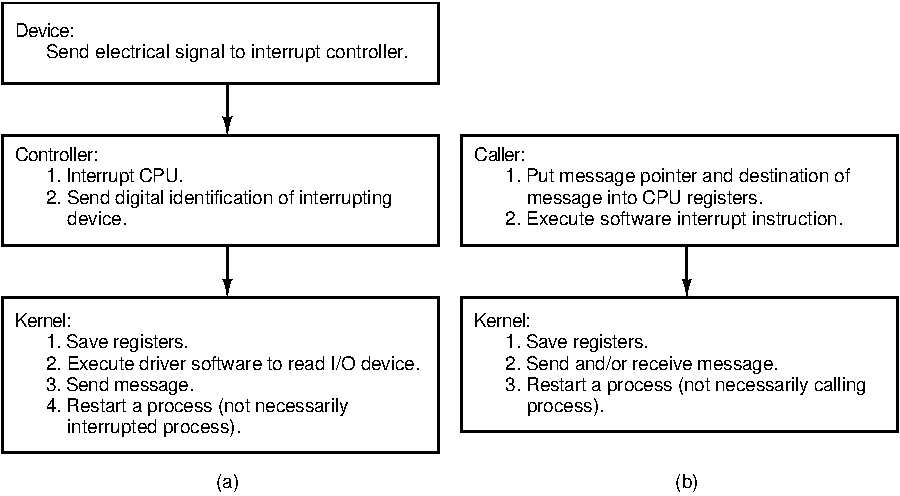
\includegraphics[width=\textwidth]{int-osdi-35}
    }
    \mode<article>{
      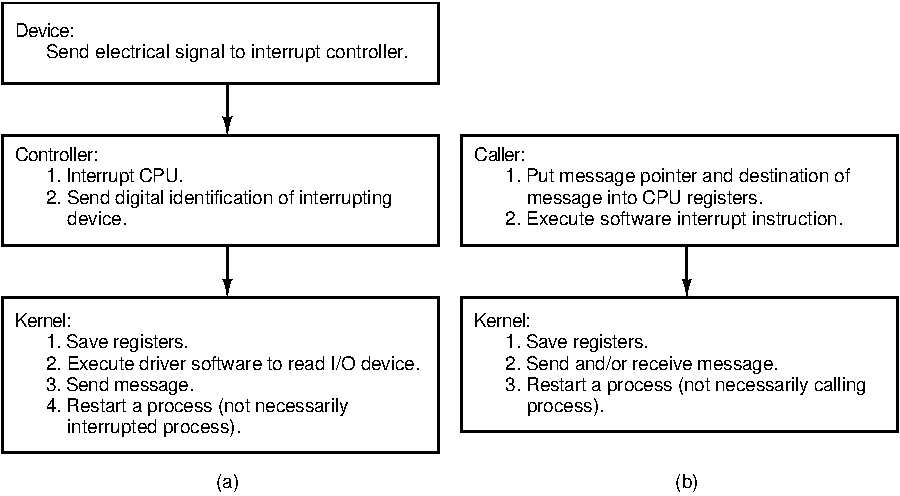
\includegraphics[width=.7\textwidth]{int-osdi-35}
    }
  \end{center}
\end{frame}

\begin{frame}\mode<beamer>{\frametitle{References}}
  \begin{refsection}
    \nocite{wiki:interrupt, wiki:syscall}
    \printbibliography[heading=subbibliography,title={References}]
  \end{refsection}
\end{frame}


\part{Process And Thread}

\lecture[proc]{proc}{proc}

\section{Processes}
\label{sec:processes}

\subsection{What's a Process}
\label{sec:whats-process}

\begin{frame}{Process}
  \begin{description}
  \item[A process] is an instance of a program in execution
  \end{description}
  \begin{minipage}{.65\linewidth}
    \begin{block}{\mbox{Processes are like human beings:}}
        \begin{itemize}
        \item[\Symbol{➠}] they are generated
        \item[\Symbol{➠}] they have a life
        \item[\Symbol{➠}] they optionally generate one or more child processes, and
        \item[\Symbol{➠}] eventually they die
        \end{itemize}
        A small difference:
        \begin{itemize}
        \item sex is not really common among processes
        \item each process has just one parent
        \end{itemize}
      \end{block}
  \end{minipage}\quad
  \begin{minipage}{.3\linewidth}
    \begin{center}
      \mode<beamer>{ 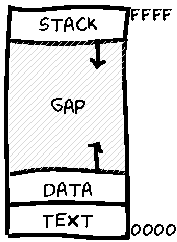
\includegraphics[width=\textwidth]{mos-figs-1-20} }%
      \mode<article>{ 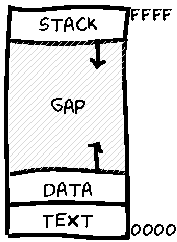
\includegraphics[width=.5\textwidth]{mos-figs-1-20} }
    \end{center}
  \end{minipage}
\end{frame}

The term "process" is often used with several different meanings. In this book, we stick
to the usual OS textbook definition: a process is an instance of a program in
execution. You might think of it as \emph{the collection of data structures that fully
  describes how far the execution of the program has progressed}. \citetitle[Sec.~3.1,
\emph{Processes, Lightweight Processes, and Threads}]{bovet2005understanding}

Processes are like human beings: they are generated, they have a more or less significant
life, they optionally generate one or more child processes, and eventually they die. A
small difference is that sex is not really common among processes each process has just
one parent.

From the kernel's point of view, the purpose of a process is to act as an entity to which
system resources (CPU time, memory, etc.) are allocated.

In general, a computer system process consists of (or is said to 'own') the following
resources \citetitle{wiki:process}:
\begin{itemize}
\item An image of the executable machine code associated with a program.
\item Memory (typically some region of virtual memory); which includes the executable
  code, process-specific data (input and output), a call stack (to keep track of active
  subroutines and/or other events), and a heap to hold intermediate computation data
  generated during run time.
\item Operating system descriptors of resources that are allocated to the process, such as
  file descriptors (Unix terminology) or handles (Windows), and data sources and sinks.
\item Security attributes, such as the process owner and the process' set of permissions
  (allowable operations).
\item Processor state (context), such as the content of registers, physical memory
  addressing, etc. The state is typically stored in computer registers when the process is
  executing, and in memory otherwise.
\end{itemize}
The operating system holds most of this information about active processes in data
structures called process control blocks.

Any subset of resource, but typically at least the processor state, may be associated with
each of the process' threads in operating systems that support threads or 'daughter'
processes.

The operating system keeps its processes separated and allocates the resources they need,
so that they are less likely to interfere with each other and cause system failures (e.g.,
deadlock or thrashing). The operating system may also provide mechanisms for inter-process
communication to enable processes to interact in safe and predictable ways.


\subsection{PCB}
\label{sec:pcb}

% 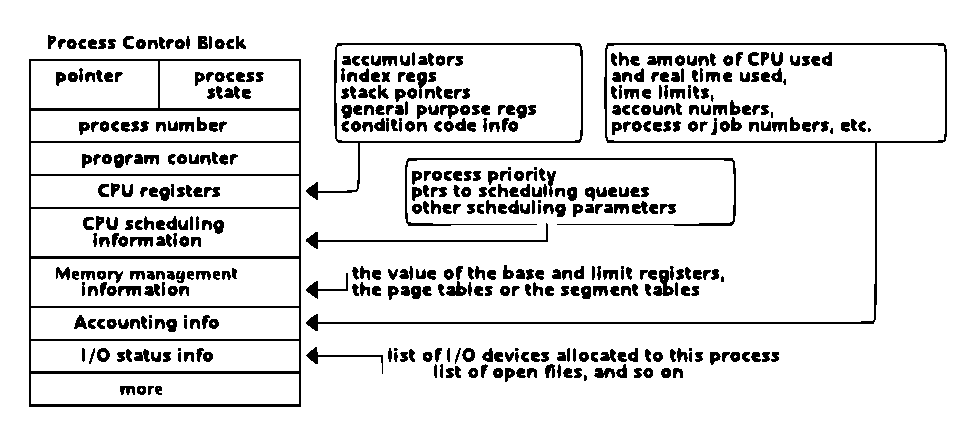
\includegraphics[width=\textwidth]{pcbpdf2}
% \includegraphics[width=\textwidth]{mos-figs-2-4}

\begin{frame}{Process Control Block (PCB)}
  \begin{varwidth}{.7\textwidth}
    \begin{block}{Implementation}
        A process is \alert{the collection of data structures} that fully describes how far
        the execution of the program has progressed.
        \begin{itemize}
        \item Each process is represented by a \alert{PCB}
        \item \texttt{task\_struct} in \linux{}
        \end{itemize}
      \end{block}
    \end{varwidth}\quad
    \begin{varwidth}{.2\textwidth}
      \begin{center}
        \mode<beamer>{
          \includegraphics[width=1.5\textwidth]{pcb}
        }
        \mode<article>{
          \includegraphics[width=\textwidth]{pcb}
        }
      \end{center}      
    \end{varwidth}
\end{frame}

To manage processes, the kernel must have a clear picture of what each process is
doing. It must know, for instance, the process's priority, whether it is running on a CPU
or blocked on an event, what address space has been assigned to it, which files it is
allowed to address, and so on. This is the role of the process descriptor a
\texttt{task\_struct} type structure whose fields contain all the information related to a
single process. As the repository of so much information, the process descriptor is rather
complex. In addition to a large number of fields containing process attributes, the
process descriptor contains several pointers to other data structures that, in turn,
contain pointers to other structures\citetitle[Sec.~3.2, \emph{Process
  Descriptor}]{bovet2005understanding}.

\subsection{Process Creation}
\label{sec:process-creation}

\begin{frame}{Process Creation}
  \begin{center}
    \mode<beamer>{ \includegraphics[width=\textwidth]{process-creation} }%
    \mode<article>{ \includegraphics[width=.5\textwidth]{process-creation} }
  \end{center}
  \begin{itemize}
  \item When a process is created, it is almost identical to its parent
    \begin{itemize}
    \item It receives a (logical) copy of the parent's address space, and
    \item executes the same code as the parent
    \end{itemize}
  \item The parent and child have separate copies of the data (stack and heap)
  \end{itemize}
\end{frame}


When a process is created, it is almost identical to its parent. It receives a (logical)
copy of the parent's address space and executes the same code as the parent, beginning at
the next instruction following the process creation system call. Although the parent and
child may share the pages containing the program code (text), they have separate copies of
the data (stack and heap), so that changes by the child to a memory location are invisible
to the parent (and vice versa)\citetitle[Sec.~3.1, \emph{Processes, Lightweight Processes, and
  Threads}]{bovet2005understanding}.

While earlier Unix kernels employed this simple model, modern Unix systems do not. They
support \emph{multi-threaded applications} user programs having many relatively
independent execution flows sharing a large portion of the application data structures. In
such systems, a process is composed of several \emph{user threads} (or simply
\emph{threads}), each of which represents an execution flow of the process. Nowadays, most
multi-threaded applications are written using standard sets of library functions called
\emph{pthread (POSIX thread) libraries}.

Traditional Unix systems treat all processes in the same way: resources owned by the
parent process are duplicated in the child process. This approach makes process creation
very slow and inefficient, because it requires copying the entire address space of the
parent process. The child process rarely needs to read or modify all the resources
inherited from the parent; in many cases, it issues an immediate \texttt{execve()} and
wipes out the address space that was so carefully copied\citetitle[Sec.~3.4, \emph{Creating
  Processes}]{bovet2005understanding}.

Modern Unix kernels solve this problem by introducing three different mechanisms:
\begin{itemize}
\item Copy On Write
\item Lightweight processes
\item The \texttt{vfork()} system call
\end{itemize}


\begin{frame}{Forking in C}
  \begin{center}
    \mode<beamer>{
      \includegraphics[width=.7\textwidth]{fork}
    } \mode<article>{
      \includegraphics[width=.4\textwidth]{fork-bw}
    }
  \end{center}
  \begin{itemize}
  \item[\$] \texttt{man fork}
  \end{itemize}
\end{frame}

\begin{frame}{\texttt{exec()}}
  \begin{center}
    \mode<beamer>{
      \includegraphics[width=.7\textwidth]{fork-exec-osc}
    } \mode<article>{
      \includegraphics[width=.4\textwidth]{fork-exec-osc-bw}
    }
  \end{center}
  \begin{itemize}
  \item[\$] \texttt{man 3 exec}
  \end{itemize}
\end{frame}

\subsection{Process State}

\begin{frame}{Process State Transition}
  \begin{center}
    \mode<beamer>{
      \includegraphics[width=\textwidth]{mos-figs-2-2}
    } \mode<article>{
      \includegraphics[width=.7\textwidth]{mos-figs-2-2}
    }
  \end{center}
\end{frame}

See also: \citetitle[Sec.~3.2.1, \emph{Process State}]{bovet2005understanding}.

\subsection{CPU Switch From Process To Process}
\label{sec:cpu-switch-from}

\begin{frame}{CPU Switch From Process To Process}
  \begin{center}
    \mode<beamer>{
      \includegraphics[width=\textwidth]{cpu-switch}
    }
    \mode<article>{
      \includegraphics[width=.7\textwidth]{cpu-switch}
    }
  \end{center}
\end{frame}

See also: \citetitle[Sec.~3.3, \emph{Process Switch}]{bovet2005understanding}.


\section{Threads}
\label{sec:threads}

\subsection{Processes vs. Threads}
\label{sec:proc-vs.-thre}

\begin{frame}{Process vs. Thread}
    \begin{tabular}{rcl}
      a single-threaded process&=&resource + execution\\
      a  multi-threaded process&=&resource + executions\\
    \end{tabular}
    \begin{center}
      \mode<beamer>{ \includegraphics[width=.7\textwidth]{mos-figs-2-6} }%
      \mode<article>{ \includegraphics[width=.6\textwidth]{mos-figs-2-6} }
    \end{center}
  \begin{description}
  \item[A process] = a unit of resource ownership, used to group resources together;
  \item[A thread] = a unit of scheduling, scheduled for execution on the CPU.
  \end{description}  
\end{frame}

\begin{frame}{Process vs. Thread}
  \begin{center}
    \begin{tabularx}{.9\textwidth}{X|X}
      \textbf{multiple threads running in one process:}&
      \textbf{multiple processes running in one computer:}\\
      share an address space and other resources&
      share physical memory, disk, printers ...\\
    \end{tabularx}
  \end{center}
  \begin{block}{No protection between threads}
    \begin{description}
    \item[impossible] --- because process is the minimum unit of resource management
    \item[unnecessary] --- a process is owned by a single user
    \end{description}    
  \end{block}
\end{frame}

\begin{frame}{Threads}
  \begin{center}
    \mode<beamer>{ \includegraphics[width=.8\textwidth]{thread-components} }%
    \mode<article>{ \includegraphics[width=.4\textwidth]{thread-components} }
  \end{center}
\end{frame}

\subsection{Why Thread?}
\label{sec:why-thread}

\begin{frame}{A Multi-threaded Web Server}\label{webserver}
  \begin{center}
    \mode<beamer>{ \includegraphics[width=.6\textwidth]{mos-figs-2-10} }%
    \mode<article>{ \includegraphics[width=.5\textwidth]{mos-figs-2-10} }
  \end{center}
  \begin{center}
    \mode<beamer>{ \includegraphics[width=\textwidth]{mos-figs-2-11} }%
    \mode<article>{ \includegraphics[width=.6\textwidth]{mos-figs-2-11} }
  \end{center}
\end{frame}

\begin{frame}{A Word Processor With 3 Threads}
  \begin{center}
    \mode<beamer>{ \includegraphics[width=\textwidth]{mos-figs-2-9} }%
    \mode<article>{ \includegraphics[width=.6\textwidth]{mos-figs-2-9} }
  \end{center}
\end{frame}

\begin{frame}{Why Having a Kind of Process Within a Process?}{}
  \begin{itemize}
  \item Responsiveness
    \begin{itemize}
    \item Good for interactive applications.
    \item A process with multiple threads makes a great server (e.g. a web server):
      \begin{itemize}
      \item[] Have one server process, many "worker" threads -- if one thread blocks (e.g. on a
        read), others can still continue executing
      \end{itemize}
    \end{itemize}
  \item Economy -- Threads are cheap!
    \begin{itemize}
    \item Cheap to create -- only need a stack and storage for registers
    \item Use very little resources -- don't need new address space, global data, program code, or
      OS resources
    \item switches are fast -- only have to save/restore PC, SP, and registers
    \end{itemize}
  \item Resource sharing -- Threads can pass data via shared memory; no need for IPC
    \item Can take advantage of multiprocessors
  \end{itemize}
\end{frame}

\subsection{Thread Characteristics}
\label{sec:thread-char}

\begin{frame}{Thread States Transition}{Same as process states transition}
  \begin{center}
    \mode<beamer>{ \includegraphics[width=\textwidth]{mos-figs-2-2} }%
    \mode<article>{ \includegraphics[width=.6\textwidth]{mos-figs-2-2} }
  \end{center}
\end{frame}

\begin{frame}{Each Thread Has Its Own Stack}
  \begin{itemize}
  \item A typical stack stores local data and call information for (usually nested) procedure
    calls. 
  \item Each thread generally has a different execution history.
  \end{itemize}
  \begin{center}
    \mode<beamer>{ \includegraphics[width=.8\textwidth]{mos-figs-2-8} }%
    \mode<article>{ \includegraphics[width=.6\textwidth]{mos-figs-2-8} }
  \end{center}
\end{frame}

\begin{frame}{Thread Operations}
  \begin{center}
    \mode<beamer>{ \includegraphics[width=.8\textwidth]{thread-operations} }%
    \mode<article>{ \includegraphics[width=.6\textwidth]{thread-operations} }
  \end{center}
\end{frame}

\subsection{POSIX Threads}
\label{sec:posix-threads}

\begin{frame}{POSIX Threads}
  \begin{description}
  \item[IEEE 1003.1c] The standard for writing portable threaded programs. The threads package it
    defines is called \alert{Pthreads}, including over 60 function calls, supported by most UNIX
    systems.
  \end{description}
  \begin{block}{Some of the Pthreads function calls}
    \begin{center}
      \begin{small}
        \begin{tabularx}{\textwidth}{>{\ttfamily}lX}
          \toprule
          \textbf{Thread call}&\textbf{Description}\\\midrule
          pthread\_create&Create a new thread\\
          pthread\_exit&Terminate the calling thread\\
          pthread\_join&Wait for a specific thread to exit\\
          pthread\_yield&Release the CPU to let another thread run\\
          pthread\_attr\_init&Create and initialize a thread's attribute structure\\
          pthread\_attr\_destroy&Remove a thread's attribute structure\\\bottomrule
        \end{tabularx}
      \end{small}
    \end{center}
  \end{block}
\end{frame}

\begin{frame}{Pthreads}{Example 1}
  \begin{center}
    \mode<beamer>{ \includegraphics[width=.75\textwidth]{thread1} }%
    \mode<article>{ \includegraphics[width=.7\textwidth]{thread1-bw} }
  \end{center}
\end{frame}

See also:
\begin{itemize}
\item IBM Developworks: POSIX threads
  explained\footnote{\url{http://www.ibm.com/developerworks/linux/library/l-posix1/index.html}}.
\item stackoverflow.com: What is the difference between \texttt{exit()} and
  \texttt{abort()}?\footnote{\url{http://stackoverflow.com/questions/397075/what-is-the-difference-between-exit-and-abort}}.
\end{itemize}

\begin{frame}{Pthreads}
  \begin{description}
  \item[\texttt{pthread\_t}] defined in \texttt{pthread.h}, is often called a "thread id"
    (\texttt{tid});
  \item[\texttt{pthread\_create()}] returns zero on success and a non-zero value on failure;
  \item[\texttt{pthread\_join()}] returns zero on success and a non-zero value on failure;
  \end{description}
  \begin{block}{How to use pthread?}
    \begin{itemize}
    \item \texttt{\#include<pthread.h>}
    \item[\$] \texttt{gcc thread1.c -o thread1 -pthread}
    \item[\$] \texttt{./thread1}
    \end{itemize}
  \end{block}
\end{frame}

\begin{frame}{Pthreads}{Example 2}
  \begin{center}
    \mode<beamer>{
      \includegraphics[width=.9\textwidth]{thread2}
    } \mode<article>{
      \includegraphics[width=.9\textwidth]{thread2-bw}
    }
  \end{center}
\end{frame}

\begin{frame}{Pthreads}
  With or without \texttt{pthread\_join()}? Check it by yourself.
\end{frame}

\subsection{User-Level Threads vs. Kernel-level Threads}
\label{sec:user-threads-vs}

\begin{frame}{User-Level Threads vs. Kernel-Level Threads}
  \begin{center}
    \mode<beamer>{
      \includegraphics[width=\textwidth]{mos-figs-2-13}
    }
    \mode<article>{
      \includegraphics[width=.6\textwidth]{mos-figs-2-13}
    }
  \end{center}
\end{frame}

\begin{frame}{User-Level Threads}
  \begin{description}
  \item[User-level threads] provide a library of functions to allow user processes to create and
    manage their own threads.
  \end{description}
  \begin{itemize}
  \item[\good] No need to modify the OS\\[-.5ex]
  \item[\good] Simple representation\\[-.5ex]
    \begin{itemize}
    \item each thread is represented simply by a PC, regs, stack, and a small TCB, all
        stored in the user process' address space
    \end{itemize}
  \item[\good] Simple Management\\[-.5ex]
    \begin{itemize}
    \item creating a new thread, switching between threads, and synchronization between threads can
      all be done without intervention of the kernel
    \end{itemize}
  \item[\good] Fast\\[-.5ex]
    \begin{itemize}
    \item thread switching is not much more expensive than a procedure call
    \end{itemize}
  \item[\good] Flexible\\[-.5ex]
    \begin{itemize}
    \item CPU scheduling (among threads) can be customized to suit the needs of the algorithm --
      each process can use a different thread scheduling algorithm
    \end{itemize}
  \end{itemize}
\end{frame}

\begin{frame}{User-Level Threads}
  \begin{itemize}
  \item[\alert{\bad}]  Lack of coordination between threads and OS kernel
    \begin{itemize}
    \item Process as a whole gets one time slice
    \item Same time slice, whether process has 1 thread or 1000 threads
    \item Also -- up to each thread to relinquish control to other threads in that process
    \end{itemize}
  \item[\alert{\bad}] Requires non-blocking system calls (i.e. a multithreaded kernel)
    \begin{itemize}
    \item Otherwise, entire process will blocked in the kernel, even if there are runnable threads
      left in the process
    \item part of motivation for user-level threads was not to have to modify the OS
    \end{itemize}
  \item[\alert{\bad}] If one thread causes a page fault(interrupt!), the entire process
    blocks
  \end{itemize}
\end{frame}

See also: \emph{More about blocking and non-blocking calls}\footnote{\url{http://www.daniweb.com/software-development/computer-science/threads/384575/synchronous-vs-asynchronous-blocking-vs-non-blocking}}.

\begin{frame}{Kernel-Level Threads}
  \begin{description}
  \item[Kernel-level threads] kernel provides system calls to create and manage threads
  \end{description}
  \begin{itemize}
  \item[\good] Kernel has full knowledge of all threads
    \begin{itemize}
    \item Scheduler may choose to give a process with 10 threads more time than process with only 1
      thread
    \end{itemize}
  \item[\good] Good for applications that frequently block (e.g. server processes with
    frequent interprocess communication)
  \item[\alert{\bad}] Slow -- thread operations are 100s of times slower than for
    user-level threads
  \item[\alert{\bad}] Significant overhead and increased kernel complexity -- kernel must
    manage and schedule threads as well as processes
    \begin{itemize}
    \item Requires a full thread control block (TCB) for each thread
    \end{itemize}
  \end{itemize}
\end{frame}

\begin{frame}{Hybrid Implementations}{Combine the advantages of two}
  \begin{center}
    \mode<beamer>{
      \includegraphics[width=.9\textwidth]{mos-figs-2-14}
    }
    \mode<article>{
      \includegraphics[width=.5\textwidth]{mos-figs-2-14}
    }
  \end{center}
\end{frame}

% \begin{frame}{Two-Level Thread Model}{Digital UNIX, Solaris, IRIX, HP-UX}
%   \begin{center}
%     \includegraphics[width=\textwidth]{thread-walker}
%   \end{center}
% \end{frame}

% \begin{frame}{Two-Level Thread Model}{Digital UNIX, Solaris, IRIX, HP-UX}
%   \begin{itemize}
%   \item User-level threads for user processes
%     \begin{itemize}
%     \item Lightweight process (LWP) serves as a "virtual CPU" where user threads can run
%     \end{itemize}
%   \item Kernel-level threads for use by kernel
%     \begin{itemize}
%     \item One for each LWP
%     \item Others perform tasks not related to LWPs
%     \item OS supports multiprocessor systems
%     \end{itemize}
%   \end{itemize}
% \end{frame}

\begin{frame}{Programming Complications}
  \begin{itemize}
  \item \texttt{fork()}: shall the child has the threads that its parent has?
  \item What happens if one thread closes a file while another is still reading from it?
  \item What happens if several threads notice that there is too little memory?
  \end{itemize}
  \alert{And sometimes, threads fix the symptom, but not the problem.}
\end{frame}

\subsection{Linux Threads}
\label{sec:linux-threads}

\begin{frame}{Linux Threads}
  \begin{block}{To the Linux kernel, there is no concept of a thread}
    \begin{itemize}
    \item Linux implements all threads as standard processes
    \item To Linux, a thread is merely a process that shares certain resources with other
      processes
    \item Some OS (MS Windows, Sun Solaris) have cheap threads and expensive processes.
    \item Linux processes are already quite lightweight
      \begin{itemize}
      \item[] On a 75MHz Pentium
        \begin{tabular}{r}
          thread: $1.7\mu{}s$\\
          fork: $1.8\mu{}s$
        \end{tabular}
      \end{itemize}
    \end{itemize}
  \end{block}
\end{frame}


\citetitle[Sec.~3.1, \emph{Processes, Lightweight Processes, and
  Threads}]{bovet2005understanding} Older versions of the Linux kernel offered no support
for multithreaded applications. From the kernel point of view, a multithreaded application
was just a normal process. The multiple execution flows of a multithreaded application
were created, handled, and scheduled entirely in User Mode, usually by means of a
POSIX-compliant \emph{pthread} library.

However, such an implementation of multithreaded applications is not very
satisfactory. For instance, suppose a chess program uses two threads: one of them controls
the graphical chessboard, waiting for the moves of the human player and showing the moves
of the computer, while the other thread ponders the next move of the game. While the first
thread waits for the human move, the second thread should run continuously, thus
exploiting the thinking time of the human player. However, if the chess program is just a
single process, the first thread cannot simply issue a blocking system call waiting for a
user action; otherwise, the second thread is blocked as well. Instead, the first thread
must employ sophisticated nonblocking techniques to ensure that the process remains
runnable.

Linux uses \emph{lightweight processes} to offer better support for multithreaded
applications. Basically, two lightweight processes may share some resources, like the
address space, the open files, and so on. Whenever one of them modifies a shared resource,
the other immediately sees the change. Of course, the two processes must synchronize
themselves when accessing the shared resource.

A straightforward way to implement multithreaded applications is to associate a
light-weight process with each thread. In this way, the threads can access the same set of
application data structures by simply sharing the same memory address space, the same set
of open files, and so on; at the same time, each thread can be scheduled independently by
the kernel so that one may sleep while another remains runnable. Examples of
POSIX-compliant pthread libraries that use Linux's lightweight processes are
\emph{LinuxThreads}, \emph{Native POSIX Thread Library (NPTL)}, and IBM's \emph{Next
  Generation Posix Threading Package (NGPT)}.

POSIX-compliant multithreaded applications are best handled by kernels that support
"thread groups". In Linux a \emph{thread group} is basically a set of lightweight
processes that implement a multithreaded application and act as a whole with regards to
some system calls such as \texttt{getpid()}, \texttt{kill()}, and \texttt{\_exit()}.


\begin{frame}{Linux Threads}
  \begin{itemize}
  \item[\texttt{clone()}] creates a separate process that shares the address space of the
    calling process. The cloned task behaves \emph{much like} a separate thread.
  \end{itemize}
  \begin{center}
    \includegraphics[width=.6\textwidth]{syscall}
  \end{center}
\end{frame}

\begin{frame}{\texttt{clone()}}
  \begin{center}
    \mode<beamer>{
      \includegraphics[width=\textwidth]{clone-prototype}
    } \mode<article>{
      \includegraphics[width=.8\textwidth]{clone-prototype-bw}
    }
  \end{center}
  \begin{small}
    \begin{description}
    \item[arg 1] the function to be executed, i.e. \texttt{fn(arg)}, which returns an \texttt{int};
    \item[arg 2] a pointer {\pright} a (usually malloced) memory space to be used as
      the stack for the new thread;
    \item[arg 3] a set of flags used to indicate how much the calling process is to be
      shared. In fact,
      \begin{itemize}
      \item[]  \texttt{clone(0) == fork()}
      \end{itemize}
    \item[arg 4] the arguments passed to the function.
    \end{description}
    It returns the PID of the child process or -1 on failure.
  \end{small}
  \begin{itemize}
    \item[\$] \texttt{man clone}
  \end{itemize}
\end{frame}

\begin{frame}{The \texttt{clone()} System Call}
  \begin{block}{Some flags:}
    \begin{center}
      \begin{tabular}{>{\ttfamily}ll}
        \toprule
        \textbf{flag}&\textbf{Shared}\\\midrule
        CLONE\_FS&File-system info\\
        CLONE\_VM&Same memory space\\
        CLONE\_SIGHAND&Signal handlers\\
        CLONE\_FILES&The set of open files\\\bottomrule
      \end{tabular}
    \end{center}
  \end{block}
  \begin{block}{In practice, one should try to avoid calling \texttt{clone()} directly}
    \begin{itemize}
    \item[] Instead, use a threading library (such as pthreads) which use \texttt{clone()}
      when starting a thread (such as during a call to \texttt{pthread\_create()})
    \end{itemize}
  \end{block}
\end{frame}

\begin{frame}{\texttt{clone()} Example}
  \begin{center}
    \mode<beamer>{
      \includegraphics[width=\textwidth]{clone2}
      \pause
      \begin{tikzpicture}[remember picture, overlay]
        \node [yshift=-7em,xshift=5em,rotate=-20,scale=6,text opacity=0.7,color=red] at
        (current page.center) {\Symbol{✘}};
      \end{tikzpicture}
    } \mode<article>{
      \includegraphics[width=.6\textwidth]{clone2-bw-crop}
    }
  \end{center}
\end{frame}

\begin{frame}[fragile]{Stack Grows Downwards}
\begin{ccode}
child_stack = (void**)malloc(8192) + 8192/sizeof(*child_stack);
\end{ccode}
  \mode<beamer>{
    \begin{tikzpicture}[remember picture, overlay]
      \node [yshift=-0.1em,xshift=9em,rotate=0,scale=12,text opacity=0.7,color=red] at
      (current page.center) {\Symbol{✔}};
    \end{tikzpicture}}
\end{frame}

% \begin{frame}{}{}
%   \begin{center}
%     \includegraphics[width=\textwidth]{mos-figs-2-15}
%   \end{center}
% \end{frame}

% \begin{frame}{}{}
%   \begin{center}
%     \includegraphics[width=\textwidth]{mos-figs-2-16}
%   \end{center}
% \end{frame}

% \begin{frame}{}{}
%   \begin{center}
%     \includegraphics[width=\textwidth]{mos-figs-2-17}
%   \end{center}
% \end{frame}

% \begin{frame}{}{}
%   Several systems today (QNX and Plan 9, for instance) take the stance that threads `fix the
%   symptom, but not the problem'. Rather than using threads because the OS context switch time is too
%   slow, a better approach, according to the architects of these systems, is to fix the OS. It's
%   ironic, now that even PC-hosted desktop OSes provide MMU-protected multitasking, the fashionable
%   programming model has become multiple threads running in a common address space, making debugging
%   difficult, and also making it more difficult to generate reliable code. With fast context
%   switching, existing OS services like explicitly allocated shared memory between a team of
%   cooperating processes can create a `threaded' environment, without opening the Pandora's box of
%   problems that a fully shared memory space entails.
% \end{frame}

\begin{frame}\mode<beamer>{\frametitle{References}}
  \begin{refsection}
    \nocite{wiki:process, wiki:thread, wiki:pcb}
    \printbibliography[heading=subbibliography,title={References}]
  \end{refsection}
\end{frame}

\lecture[ipc]{ipc}{ipc}

\section{Process Synchronization}
\label{sec:proc-synchr}

\subsection{IPC}
\label{sec:ipc}

\begin{frame}{Interprocess Communication}
  \begin{block}{Example:}
    \begin{itemize}
    \item[\$] \texttt{ps | head -2 | tail -1 | cut -f2 -d' '}
    \end{itemize}
  \end{block}
  \begin{block}{IPC issues:}
    \begin{enumerate}
    \item How one process can pass information to another
    \item Be sure processes do not get into each other's way
      \begin{itemize}
      \item[e.g.] in an airline reservation system, two processes compete for the last
        seat
      \end{itemize}
    \item Proper sequencing when dependencies are present
      \begin{itemize}
      \item[e.g.] if A produces data and B prints them, B has to wait until A has produced
        some data
      \end{itemize}
    \end{enumerate}
  \end{block}
  \begin{block}{Two models of IPC:}
    \begin{itemize}
    \item Shared memory
    \item Message passing (e.g. sockets)
    \end{itemize}
  \end{block}
\end{frame}

\begin{frame}{Producer-Consumer Problem}
\begin{center}
  \mode<beamer>{
    \includegraphics[width=.9\textwidth]{ipc}
  } \mode<article>{
    \includegraphics[width=.4\textwidth]{ipc-bw}
  }
\end{center}
\end{frame}

\subsection{Shared Memory}
\label{sec:shared-memory}

\begin{frame}{Process Synchronization}{Producer-Consumer Problem}
  \begin{itemize}
  \item Consumers don't try to remove objects from Buffer when it is empty.
  \item Producers don't try to add objects to the Buffer when it is full.
  \end{itemize}
  \begin{center}
    \mode<beamer>{
      \includegraphics[width=\textwidth]{producer-consumer}
    } \mode<article>{
      \includegraphics[width=.5\textwidth]{producer-consumer-bw}
    }
  \end{center}
  \begin{center}
    How to define \alert{full/empty}?
  \end{center}
\end{frame}

\begin{frame}{Producer-Consumer Problem}{--- Bounded-Buffer Problem (Circular Array)}
  \begin{minipage}{.65\linewidth}
  \begin{description}
  \item[Front(out):] the first full position
  \item[Rear(in):] the next free position
  \end{description}
  \end{minipage}\quad
  \begin{minipage}{.3\linewidth}
    \mode<beamer>{ \includegraphics[width=\textwidth]{circular} }%
    \mode<article>{ \includegraphics[width=.7\textwidth]{circular-bw} }
  \end{minipage}
  Full or empty when ``$front == rear$''?
\end{frame}

\begin{frame}{Producer-Consumer Problem}
  \begin{block}{Common solution:}
    \begin{description}
    \item[Full:] when ``$\mathtt{(in+1)\%BUFFER\_SIZE == out}$''
      \begin{itemize}
      \item[] Actually, this is ``$\mathtt{full - 1}$''
      \end{itemize}
    \item[Empty:] when ``$\mathtt{in == out}$''
    \end{description}
    Can only use ``$\mathtt{BUFFER\_SIZE-1}$'' elements
  \end{block}
  
  \begin{block}{Shared data:}
    \begin{center}
      \mode<beamer>{
        \includegraphics[width=.8\textwidth]{shared-data}
      } \mode<article>{
        \includegraphics[width=.4\textwidth]{shared-data-bw}
      }
    \end{center}
  \end{block}
\end{frame}

\begin{frame}{Bounded-Buffer Problem}
  \begin{minipage}{.7\linewidth}
    \begin{block}{Producer:}
      \begin{center}
        \mode<beamer>{
          \includegraphics[width=\textwidth]{bounded-buffer-1}
        } \mode<article>{
          \includegraphics[width=.8\textwidth]{bounded-buffer-1-bw}
        }
      \end{center}
    \end{block}
    \begin{block}{Consumer:}
      \begin{center}
        \mode<beamer>{
          \includegraphics[width=\textwidth]{bounded-buffer-2}
        } \mode<article>{
          \includegraphics[width=.8\textwidth]{bounded-buffer-2-bw}
        }
      \end{center}
    \end{block}
  \end{minipage}\hfill
  \begin{minipage}{.28\linewidth}
    \begin{center}
      \mode<beamer>{ \includegraphics[width=\textwidth]{circular} }%
      \mode<article>{ \includegraphics[width=\textwidth]{circular-bw} }
    \end{center}
  \end{minipage}
\end{frame}

\subsection{Race Condition and Mutual Exclusion}
\label{sec:race-condition}

\begin{frame}{Race Conditions}
  \begin{block}{Now, let's have two producers}
    \begin{center}
      \mode<beamer>{ \includegraphics[width=.8\textwidth]{mos-figs-2-18} }%
      \mode<article>{ \includegraphics[width=.45\textwidth]{mos-figs-2-18} }
    \end{center}
  \end{block}
\end{frame}

\begin{frame}{Race Conditions}{Two producers}
  \begin{center}
    \mode<beamer>{ \includegraphics[width=.6\textwidth]{two-producer} }%
    \mode<article>{ \includegraphics[width=.4\textwidth]{two-producer-bw} }
  \end{center}
  \begin{block}{Process A and B do the same thing:}
    \begin{center}
      \mode<beamer>{ \includegraphics[width=.8\textwidth]{two-producer-2} }%
      \mode<article>{ \includegraphics[width=.5\textwidth]{two-producer-2-bw} }
    \end{center}
  \end{block}
\end{frame}

\begin{frame}{Race Conditions}
  \begin{description}
  \item[Problem:] Process \texttt{B} started using one of the \emph{shared variables} before
    Process \texttt{A} was finished with it.
  \item[Solution:] \alert{Mutual exclusion}. If one process is using a shared variable or
    file, the other processes will be excluded from doing the same thing.
  \end{description}
\end{frame}

\begin{frame}{Critical Regions}{Mutual Exclusion}
  \begin{description}
  \item[Critical Region:] is a piece of code accessing a common resource.
  \end{description}
  \begin{center}
    \mode<beamer>{ \includegraphics[width=\textwidth]{mos-figs-2-19} }%
    \mode<article>{ \includegraphics[width=.7\textwidth]{mos-figs-2-19} }
  \end{center}
\end{frame}

\begin{frame}[label=cond]{Critical Region}
  A solution to the critical region problem must satisfy three conditions:
  \begin{description}
  \item[Mutual Exclusion:] No two process may be simultaneously inside their critical regions.
  \item[Progress:] No process running outside its critical region may block other processes.
  \item[Bounded Waiting:] No process should have to wait forever to enter its critical region.
  \end{description}
\end{frame}

\begin{frame}{Mutual Exclusion With Busy Waiting}{Disabling Interrupts}
  \begin{minipage}{.3\linewidth}
    \mode<beamer>{ \includegraphics[width=\textwidth]{disable-int} }%
    \mode<article>{ \includegraphics[width=\textwidth]{disable-int} }
  \end{minipage}\quad
  \begin{minipage}{.65\linewidth}
    \begin{block}{Problems:}
      \begin{itemize}
      \item It's not wise to give user process the power of turning off INTs.
        \begin{itemize}
        \item Suppose one did it, and never turned them on again
        \end{itemize}
      \item useless for multiprocessor system
      \end{itemize}
    \end{block}
  \end{minipage}\\[1em]
  Disabling INTs is often a useful technique within the kernel itself but is not a general
  mutual exclusion mechanism for user processes.
\end{frame}

\begin{frame}{Mutual Exclusion With Busy Waiting}{Lock Variables}
  \begin{minipage}{.45\linewidth}
    \mode<beamer>{ \includegraphics[width=\textwidth]{lock-var} }%
    \mode<article>{ \includegraphics[width=\textwidth]{lock-var-bw} }
  \end{minipage}\quad
  \begin{minipage}{.5\linewidth}
    \begin{block}{Problem:}
      \begin{itemize}
      \item What if an interrupt occurs right at line 5?
      \item Checking the lock again while backing from an interrupt?
      \end{itemize}
    \end{block}
  \end{minipage}
\end{frame}

\begin{frame}{Mutual Exclusion With Busy Waiting}{Strict Alternation}
  \begin{center}
    \mode<beamer>{ \includegraphics[width=\textwidth]{strict-alternation} }%
    \mode<article>{ \includegraphics[width=.5\textwidth]{strict-alternation-bw} }
  \end{center}
  \begin{block}{Problem: violates \hyperlink{cond}{condition-2}}
    \begin{itemize}
    \item One process can be blocked by another not in its critical region.
    \item Requires the two processes strictly alternate in entering their critical region.
    \end{itemize}
  \end{block}
\end{frame}

\begin{frame}{Mutual Exclusion With Busy Waiting}{Peterson's Solution}
  \begin{center}
    \mode<beamer>{
      \includegraphics[width=\textwidth]{peterson}
    } \mode<article>{
      \includegraphics[width=.6\textwidth]{peterson-bw}
    }
  \end{center}
  \begin{refsection}
    \nocite{wiki:peterson}
    \printbibliography[heading=subbibliography,title={References}]
  \end{refsection}
\end{frame}

\begin{frame}{Mutual Exclusion With Busy Waiting}{Hardware Solution: The TSL Instruction}
  \begin{block}{Lock the memory bus}
    \begin{center}
      \mode<beamer>{
        \includegraphics[width=\textwidth]{mos-figs-2-22}
      } \mode<article>{
        \includegraphics[width=.6\textwidth]{mos-figs-2-22}
      }
    \end{center}
  \end{block}
\end{frame}

See also: \citetitle[Sec.~2.3.3, \emph{Mutual Exclusion With Busy Waiting},
p.~124]{tanenbaum2008modern}.

\begin{frame}{Mutual Exclusion Without Busy Waiting}{Sleep \& Wakeup}
  % \includegraphics[width=.7\textwidth]{mos-figs-2-23}
  \begin{center}
    \mode<beamer>{
      \includegraphics[width=\textwidth]{sleep-wakeup}\pause
      \begin{tikzpicture}[remember picture, overlay]
        \node [rotate=10,scale=5,text opacity=0.5,color=red] at (current page.center)
        {Deadlock!};
      \end{tikzpicture}
    } \mode<article>{
      \includegraphics[width=.7\textwidth]{sleep-wakeup-bw-crop}
    }
  \end{center}
\end{frame}

\begin{frame}{Producer-Consumer Problem}{Race Condition}
  \begin{block}{Problem}
    \begin{enumerate}
    \item Consumer is going to sleep upon seeing an empty buffer, but INT occurs;
    \item Producer inserts an item, increasing \texttt{count} to \texttt{1}, then call
      \texttt{wakeup(consumer)};
    \item But the consumer is not asleep, though \texttt{count} was \texttt{0}. So \emph{the
        \texttt{wakeup()} signal is lost};
    \item Consumer is back from INT remembering \texttt{count} is \texttt{0}, and goes to
      sleep;
    \item Producer sooner or later will fill up the buffer and also goes to sleep;
    \item Both will sleep forever, and waiting to be waken up by the other
      process. Deadlock!
    \end{enumerate}
  \end{block}
\end{frame}

\begin{frame}{Producer-Consumer Problem}{Race Condition}
  \begin{block}{Solution: Add a \emph{wakeup waiting bit}}
    \begin{enumerate}
    \item The bit is set, when a wakeup is sent to an awaken process;
    \item Later, when the process wants to sleep, it checks the bit first. Turns it off if it's set,
      and stays awake.
    \end{enumerate}
    What if many processes try going to sleep?
  \end{block}
\end{frame}

\subsection{Semaphores}
\label{sec:semaphores}

\begin{frame}[fragile,squeeze]{What is a Semaphore?\,\includegraphics[width=1em]{semaphore-papa}}
  \begin{itemize}
  \item A locking mechanism
  \item An integer or ADT\\[1em]
  \end{itemize}
  \begin{minipage}{.42\linewidth}
    \begin{small}{\ttfamily
      \begin{tabular}{ll}\toprule
        \multicolumn2{c}{\emph{Atomic} Operations}\\\midrule
        P()         &V()\\
        Wait()      &Signal()\\
        Down()      &Up()\\
        Decrement() &Increment()\\
        ...         &...\\\bottomrule
      \end{tabular}}
    \end{small}
  \end{minipage}\quad
  \begin{minipage}{.53\linewidth}
    \mode<beamer>{ \includegraphics[width=\textwidth]{down-up} }%
    \mode<article>{ \includegraphics[width=\textwidth]{down-up-bw} }
  \end{minipage}
  \begin{block}{More meaningful names:}
    \begin{itemize}
    \item \texttt{increment\_and\_wake\_a\_waiting\_process\_if\_any()}
    \item \texttt{decrement\_and\_block\_if\_the\_result\_is\_negative()}
    \end{itemize}
  \end{block}
\end{frame}

\begin{frame}{Semaphore\,\includegraphics[width=1em]{semaphore-papa}}%{P/V, Down/Up, Wait/Signal...}
\begin{block}{How to ensure atomic?}
  \begin{enumerate}
  \item For single CPU, implement \texttt{up()} and \texttt{down()} as system calls, with the
    OS disabling all interrupts while accessing the semaphore;
  \item For multiple CPUs, to make sure only one CPU at a time examines the semaphore, a lock
    variable should be used with the TSL instructions.
  \end{enumerate}
\end{block}
\end{frame}

\begin{frame}{Semaphore is a Special Integer\,\includegraphics[width=1em]{semaphore-papa}}
  \begin{block}{A semaphore is like an integer, with three differences:}
    \begin{enumerate}
    \item You can initialize its value to any integer, but after that the only operations you are
      allowed to perform are \emph{increment} (\texttt{S++}) and \emph{decrement} (\texttt{S-\,-}).
    \item When a thread decrements the semaphore, if the result is negative
      ($\mathtt{S\le{}0}$), the thread blocks itself and cannot continue until another
      thread increments the semaphore.
    \item When a thread increments the semaphore, if there are other threads waiting, one of the
      waiting threads gets unblocked.
    \end{enumerate}
  \end{block}
\end{frame}

\begin{frame}{Why Semaphores?\,\includegraphics[width=1em]{semaphore-papa}}
  We don't need semaphores to solve synchronization problems, but there are some advantages to using
  them:
  \begin{itemize}
  \item Semaphores impose deliberate constraints that help programmers avoid errors.
  \item Solutions using semaphores are often clean and organized, making it easy to demonstrate
    their correctness.
  \item Semaphores can be implemented efficiently on many systems, so solutions that use semaphores
    are portable and usually efficient.
  \end{itemize}
\end{frame}

\begin{frame}{The Simplest Use of Semaphore}{Signaling}
  \begin{itemize}
  \item One thread sends a signal to another thread to indicate that something has
    happened
  \item it solves the serialization problem
    \begin{itemize}
    \item[] Signaling makes it possible to guarantee that a section of code in one thread
      will run before a section of code in another thread
    \end{itemize}
  \end{itemize}
  \begin{center}
    \mode<beamer>{
      \includegraphics[width=.7\textwidth]{sem-signaling}
    } \mode<article>{
      \includegraphics[width=.4\textwidth]{sem-signaling}
    }
  \end{center}
  \begin{center}
    What's the initial value of \texttt{sem}?
  \end{center}
\end{frame}

\begin{frame}{Semaphore}{Rendezvous Puzzle}
  \begin{center}
    \mode<beamer>{
      \includegraphics[width=.8\textwidth]{rendezvous}
    } \mode<article>{
      \includegraphics[width=.4\textwidth]{rendezvous}
    }
  \end{center}
  \begin{itemize}
  \item[Q:] How to guarantee that
    \begin{enumerate}
    \item \texttt{a1} happens before \texttt{b2}, and
    \item \texttt{b1} happens before \texttt{a2}
    \end{enumerate}
    \texttt{a1} $\rightarrow{}$ \texttt{b2};\quad \texttt{b1} $\rightarrow{}$ \texttt{a2}
  \item[Hint:] Use two semaphores initialized to 0.
  \end{itemize}
\end{frame}

\begin{frame}[fragile]
  \begin{center}
    \begin{tabular}{rp{.35\textwidth}p{.35\textwidth}}\toprule
      &\textbf{Thread A:}&\textbf{Thread B:}\\\midrule
      Solution 1:& \begin{minipage}[m]{\linewidth}
                     \begin{pythoncode}
statement a1
sem1.wait()  
sem2.signal()
statement a2 
\end{pythoncode}
                   \end{minipage}
                         & \begin{minipage}[m]{\linewidth}
\begin{pythoncode}
statement b1
sem1.signal()
sem2.wait()
statement b2 
\end{pythoncode}
                         \end{minipage}\\
      &&\\
      &&\\
      Solution 2:& \begin{minipage}[m]{\linewidth}
\begin{pythoncode}
statement a1 
sem2.signal()
sem1.wait()  
statement a2 
\end{pythoncode}
                   \end{minipage}
                         & \begin{minipage}[m]{\linewidth}
\begin{pythoncode}
statement b1
sem1.signal()
sem2.wait()
statement b2 
\end{pythoncode}
                         \end{minipage} \\
      &&\\
      &&\\
      Solution 3:& \begin{minipage}[m]{\linewidth}
\begin{pythoncode}
statement a1 
sem2.wait()  
sem1.signal()
statement a2 
\end{pythoncode}
                   \end{minipage}
                         & \begin{minipage}[m]{\linewidth}
\begin{pythoncode}
statement b1
sem1.wait()
sem2.signal()
statement b2 
\end{pythoncode}
                           \end{minipage}\\\bottomrule
    \end{tabular}
  \end{center}
  \mode<beamer>{\pause
    \begin{tikzpicture}[remember picture, overlay]
      \node [rotate=10,scale=3,opacity=0.5,color=red,anchor=south,yshift=2.5ex] at
      (current page.south) {Deadlock!};
    \end{tikzpicture}
  } \mode<article>{ \alert{Solution 3 has deadlock!}  }
\end{frame}

\begin{frame}
  \begin{block}{Mutex}
    \begin{itemize}
    \item A second common use for semaphores is to enforce \underline{mut}ual
      \underline{ex}clusion
    \item It guarantees that only one thread accesses the shared variable at a time
    \item A \texttt{mutex} is like a token that passes from one thread to another, allowing
      one thread at a time to proceed
    \end{itemize}
  \end{block}
  \begin{itemize}
  \item[Q:] Add semaphores to the following example to enforce mutual exclusion to the
    shared variable \texttt{i}.
  \end{itemize}
  \begin{multicols}{2}
    \begin{description}
    \item[Thread A:] \cfbox{violet}{\texttt{i++}}
    \item[Thread B:] \cfbox{violet}{\texttt{i++}}
    \end{description}
  \end{multicols}
  \begin{description}
  \item[Why?] Because \texttt{i++} is not atomic.
  \end{description}
\end{frame}

\begin{frame}%{\texttt{i++} is Not Thread Safe}
  \begin{block}{\texttt{i++} is not atomic in assembly language}
    \begin{center}
      \mode<beamer>{
        \includegraphics[width=.8\textwidth]{ipp}
      } \mode<article>{
        \includegraphics[width=.5\textwidth]{ipp-bw}
      }
    \end{center}
  \end{block}
  Interrupts might occur in between. So, \texttt{i++} needs to be protected with a \texttt{mutex}.
\end{frame}

\begin{frame}{Mutex Solution}
  \begin{block}{Create a semaphore named \texttt{mutex} that is initialized to
      \texttt{1}}
    \begin{itemize}
    \item[1:] a thread may proceed and access the shared variable
    \item[0:] it has to wait for another thread to release the mutex
    \end{itemize}
  \end{block}
  \begin{center}
    \mode<beamer>{
      \includegraphics[width=.8\textwidth]{mutex-ipp}
    } \mode<article>{
      \includegraphics[width=.5\textwidth]{mutex-ipp}
    }
  \end{center}
\end{frame}

\begin{frame}[label=comp,fragile]{Multiplex --- Without Busy Waiting}
  \begin{center}
    \mode<beamer>{
      \includegraphics[width=.7\textwidth]{sem-multiplex}
    } \mode<article>{
      \includegraphics[width=.5\textwidth]{sem-multiplex-bw}
    }
  \end{center}
  \vskip -1ex
  {\ttfamily
    \begin{itemize}
    \item[if] S.space < 0,\\
      S.space == Number of queuing producers
    \item[if] S.space > 5,\\
      S.space == Number of queuing consumers + 5
    \end{itemize}}
\end{frame}

\paragraph{The work flow}

There are several processes running simultaneously. They all need to
access some common resources.
\begin{enumerate}
\item Assuming \texttt{S.space == 3} in the beginning
\item Process P1 comes and take one resource away. \texttt{S.space == 2} now.
\item Process P2 comes and take the 2nd resource away. \texttt{S.space == 1} now.
\item Process P3 comes and take the last resource away. \texttt{S.space == 0} now.
\item Process P4 comes and sees nothing left. It has to sleep. \texttt{S.space == -1} now.
\item Process P5 comes and sees nothing left. It has to sleep. \texttt{S.space == -2} now.
\item At this moment, there are 2 processes (P4 and P5) sleeping. In another word, they
  are queuing for resources.
\item Now, P1 finishes using the resource, and released it. After it does a
  \texttt{S.space++}, it finds out that \texttt{S.space <= 0}. So it wakes up a Process
  (say P4) in the queue.
\item P4 wakes up, and back to execute the instruction right after \texttt{sleep()}.
\item P4 (or P2|P3) finishes using the resource, and releases it. After it does a
  \texttt{S.space++}, it finds out that \texttt{S.space <= 0}. So it wakes up P5 in the
  queue.
\item the queue is empty now.
\end{enumerate}

\begin{frame}{Barrier}
  % the little book of semaphores
  \begin{center}
    \mode<beamer>{
      \includegraphics[width=.7\textwidth]{barrier}
    }
    \mode<article>{
      \includegraphics[width=.6\textwidth]{barrier}
    }
  \end{center}
  \begin{enumerate}
  \item Processes approaching a barrier
  \item All processes but one blocked at the barrier
  \item When the last process arrives at the barrier, all of them are let through
  \end{enumerate}
  \begin{block}{Synchronization requirement:}
    \begin{center}
      \begin{tabular}{l}
        \texttt{specific\_task()}\\
        \texttt{critical\_point()}
      \end{tabular}
    \end{center}
    No thread executes \texttt{critical\_point()} until after all threads have executed
    \texttt{specific\_task()}.
  \end{block}
\end{frame}

\begin{frame}{Barrier Solution}
  \begin{center}
    \mode<beamer>{
      \includegraphics[width=.45\textwidth]{barrier-1}
    } \mode<article>{
      \includegraphics[width=.4\textwidth]{barrier-1}
    }
  \end{center}
  \begin{small}
    \begin{itemize}
    \item[count:] keeps track of how many threads have arrived
    \item[mutex:] provides exclusive access to \texttt{count}
    \item[barrier:] is locked ($\le 0$) until all threads arrive%; then it should be
      %unlocked ($\ge 1$)
    \end{itemize}
    When \texttt{barrier.value<0},
    \begin{center}
      \texttt{barrier.value == Number of queueing processes}
    \end{center}
  \end{small}
  \begin{center}
    \mode<beamer>{
      \includegraphics[width=.8\textwidth]{barrier-2}
    } \mode<article>{
      \includegraphics[width=.5\textwidth]{barrier-2-bw}
    }
  \end{center}
  \pause
  \begin{center}
    \alert{Only one thread can pass the barrier!}
  \end{center}
  \mode<beamer>{
    \begin{tikzpicture}[remember picture, overlay]
      \node [scale=10,text opacity=0.3,color=red,yshift=-.8em,xshift=-.4em] at (current
      page.center) {\Symbol{✔}};

      \node [scale=2.2,text opacity=0.3,color=red,yshift=-3em,xshift=3em,rotate=20] at
      (current page.center) {Deadlock!};
    \end{tikzpicture}
  }
\end{frame}

\begin{frame}{Barrier Solution}
  \begin{center}
    \mode<beamer>{
      \includegraphics[width=\textwidth]{barrier-3}
    } \mode<article>{
      \includegraphics[width=.5\textwidth]{barrier-3-bw}
    }
  \end{center}
  \mode<beamer>{
    \pause
    \begin{center}
      {\color{red}\danger{}} \alert{Blocking on a semaphore while holding a
        mutex!} {\color{red}\danger{}} 
    \end{center}
    \begin{tikzpicture}[remember picture, overlay]
      \node [rotate=40,scale=3.5,text opacity=0.3,color=red,xshift=2.2em,yshift=-1em] at
      (current page.center) {Deadlock!};
    \end{tikzpicture}
  }
  \mode<article>{
    \begin{center}
      \danger{} Blocking on a semaphore while holding a mutex!\danger{}
    \end{center}
  }
\end{frame}

\begin{frame}%{Barrier Solution}
  \begin{center}
    \begin{tabular}{l}
      \texttt{barrier.wait();}\\
      \texttt{barrier.signal();}
    \end{tabular}
  \end{center}
  \begin{block}{Turnstile}
    This pattern, a \texttt{wait} and a \texttt{signal} in rapid succession, occurs often
    enough that it has a name called a \emph{turnstile}, because
    \begin{itemize}
    \item it allows one thread to pass at a time, and
    \item it can be locked to bar all threads
    \end{itemize}
  \end{block}
\end{frame}

\begin{frame}{Semaphores}{Producer-Consumer Problem}
  \begin{block}{Whenever an event occurs}
    \begin{itemize}
    \item a producer thread creates an \emph{event object} and adds it to the event
      buffer. Concurrently,
    \item consumer threads take events out of the buffer and process them. In this case,
      the consumers are called ``\emph{event handlers}''.
    \end{itemize}
  \end{block}
  \begin{center}
    \mode<beamer>{
      \includegraphics[width=.9\textwidth]{event}
    } \mode<article>{
      \includegraphics[width=.5\textwidth]{event-bw}
    }
  \end{center}
  \begin{itemize}
  \item[Q:] Add synchronization statements to the producer and consumer code to enforce
    the synchronization constraints
    \begin{enumerate}
    \item Mutual exclusion
    \item Serialization
    \end{enumerate}
  \end{itemize}
\end{frame}

See also: \citetitle[Sec.~4.1, \emph{Producer-Consumer Problem}]{downey2008semaphores}.

\begin{frame}{Semaphores --- Producer-Consumer Problem}{Solution}
  \begin{block}{Initialization:}
    \begin{center}
      \begin{tabular}{>{\ttfamily}l}
        mutex = Semaphore(1)\\
        items = Semaphore(0)
      \end{tabular}
    \end{center}
    \begin{itemize}
    \item \texttt{mutex} provides exclusive access to the buffer
    \item \texttt{items}:
      \begin{itemize}
      \item[{\nerd }] number of items in the buffer
      \item[{\nerd }] number of consumer threads in queue
      \end{itemize}
    \end{itemize}
  \end{block}
\end{frame}

\begin{frame}{Semaphores --- Producer-Consumer Problem}{Solution}
  \begin{center}
    \mode<beamer>{ \includegraphics[width=\textwidth]{event-2} }%
    \mode<article>{ \includegraphics[width=.5\textwidth]{event-2-bw} }
  \end{center}
  
  \mode<article>{
    \begin{itemize}
    \item[\danger{}] any time you wait for a semaphore while holding a mutex!
    \end{itemize}}
  \mode<beamer>{\pause    
    \begin{itemize}
    \item[{\color{red}\danger{}}] any time you wait for a semaphore while holding a mutex!
    \end{itemize}
    \begin{tikzpicture}[remember picture, overlay]
      \node [rotate=15,scale=2.5,text opacity=0.4,color=red,yshift=-3em,xshift=2.5em] at
      (current page.center) {Deadlock!};
    \end{tikzpicture}}
\end{frame}

\begin{minipage}{.4\linewidth}
\begin{ccode}
  items.signal()
  {
    items++;
    if(items == 0)
      wakeup(consumer);
  }  
\end{ccode} 
\end{minipage}
\qquad\qquad
\begin{minipage}{.4\linewidth}
\begin{ccode}
  items.wait()
  {
    items--;
    if(items < 0)
      sleep();
  }
\end{ccode} 
\end{minipage}

\begin{frame}{Producer-Consumer Problem With Bounded-Buffer}
  \begin{block}{Given:}
    \begin{center}
      \begin{tabular}{>{\ttfamily}l}
        semaphore items = 0;\\
        semaphore spaces = BUFFER\_SIZE;
      \end{tabular}
    \end{center}
  \end{block}
  \begin{block}{Can we?}
    \begin{center}
      \begin{tabular}{>{\ttfamily}r}
        if (items >= BUFFER\_SIZE)\\
        producer.block();
      \end{tabular}
    \end{center}
    \begin{description}
    \item[if:] the buffer is full
    \item[then:] the producer blocks until a consumer removes an item
    \end{description}
  \end{block}
  \pause 
  \alert{No!} We can't check the current value of a semaphore, because
  \begin{itemize}
  \item[!] \alert{the only operations are \texttt{wait} and \texttt{signal}}.
  \item[?] \hyperlink{comp}{But...}
  \end{itemize}
  \mode<beamer>{
    \begin{tikzpicture}[remember picture, overlay]
      \node [rotate=-20,scale=3,text opacity=0.7,color=red,yshift=0em,xshift=.7em] at
      (current page.center) {\Symbol{✘}};
    \end{tikzpicture}
  }
\end{frame}

\paragraph{Why can't check the current value of a semaphore?}

We DO have seen:
  
\begin{minipage}{.4\linewidth}
  \begin{ccode}
void S.down(){
  S.value--;
  if(S.value < 0){
    addToQueue(S.L);
    sleep();
  }
}      
\end{ccode}
\end{minipage}
\qquad
\begin{minipage}{.4\linewidth}
  \begin{ccode}
void S.up(){
  S.value++;
  if(S.value <= 0){
    rmFromQueue(S.L);
    wakeup(S.L);
  }
}    
  \end{ccode}
\end{minipage}

Notice that the checking is within \texttt{down()} and \texttt{up()}, and is not available to
user process to use it directly.

\begin{frame}{Producer-Consumer Problem With Bounded-Buffer}
  \begin{center}
    \mode<beamer>{
      \includegraphics[width=\textwidth]{sem-putintobuf}
    } \mode<article>{
      \includegraphics[width=.6\textwidth]{sem-putintobuf-bw}
    }
  \end{center}
  \pause
  \begin{itemize}
  \item[] works fine when there is only one producer and one consumer, because
      \texttt{putIntoBuffer()} is not atomic.
  \end{itemize}
  \mode<beamer>{
    \begin{tikzpicture}[remember picture, overlay]
      \node [rotate=-20,scale=15,text opacity=0.7,color=red,yshift=0em,xshift=0em] at
      (current page.center) {!};
    \end{tikzpicture}
  }
\end{frame}

\begin{frame}%{Producer-Consumer Problem With Bounded-Buffer}
  \begin{block}{\texttt{putIntoBuffer()} could contain two actions:}
    \begin{enumerate}
    \item determining the next available slot
    \item writing into it
    \end{enumerate}
  \end{block}
  \begin{block}{Race condition:}
    \begin{enumerate}
    \item Two producers decrement spaces
    \item One of the producers determines the next empty slot in the buffer
    \item Second producer determines the next empty slot and gets the same result as the
      first producer
    \item Both producers write into the same slot
    \end{enumerate}
  \end{block}
  \texttt{putIntoBuffer()} needs to be protected with a \texttt{mutex}.
\end{frame}

\begin{frame}{With a \texttt{mutex}}%{Producer-Consumer Problem With Bounded-Buffer}
  \begin{center}
    \mode<beamer>{
      \includegraphics[width=\textwidth]{putintobuf-2}
    } \mode<article>{
      \includegraphics[width=.6\textwidth]{putintobuf-2-bw}
    }
  \end{center}
\end{frame}

\subsection{Monitors}
\label{sec:monitors}

\begin{frame}{Monitors}
  \begin{description}
  \item[Monitor] a high-level synchronization object for achieving mutual exclusion.
  \end{description}
  \begin{minipage}{.6\linewidth}
    \begin{itemize}
    \item It's a language concept, and C does not have it.
    \item Only one process can be active in a monitor at any instant.
    \item It is up to the compiler to implement mutual exclusion on monitor entries.
      \begin{itemize}
      \item The programmer just needs to know that by turning all the critical regions
        into monitor procedures, no two processes will ever execute their critical regions
        at the same time.
      \end{itemize}
    \end{itemize}
  \end{minipage}
  \hfill
  \begin{minipage}{.39\linewidth}
    \begin{center}
      \mode<beamer>{
        \includegraphics[width=\textwidth]{monitor}
      } \mode<article>{
        \includegraphics[width=\textwidth]{monitor-bw}
      }
    \end{center}
  \end{minipage}
\end{frame}

\begin{frame}{Monitor}{The producer-consumer problem}
  \begin{center}
    \mode<beamer>{
      \includegraphics[width=\textwidth]{monitor-2}
    } \mode<article>{
      \includegraphics[width=.6\textwidth]{monitor-2-bw}
    }
  \end{center}
\end{frame}

\subsection{Message Passing}
\label{sec:message-passing}  

\begin{frame}{Message Passing}
  \begin{itemize}
  \item Semaphores are too low level
  \item Monitors are not usable except in a few programming languages
  \item Neither monitor nor semaphore is suitable for distributed systems
  \item No conflicts, easier to implement
  \end{itemize}
  Message passing uses two primitives, \texttt{send} and \texttt{receive} system calls:
  \begin{itemize}
  \item[-] \texttt{send(destination,\ \&message);}
  \item[-] \texttt{receive(source, \ \&message);}
  \end{itemize}
\end{frame}

\begin{frame}{Message Passing}
  \begin{block}{Design issues}
    \begin{itemize}
    \item Message can be lost by network; --- \texttt{ACK}
    \item What if the ACK is lost? --- \texttt{SEQ}
    \item What if two processes have the same name? --- \texttt{socket}
    \item Am I talking with the right guy? Or maybe a MIM? --- \texttt{authentication}
    \item What if the sender and the receiver on the same machine? --- Copying messages is
      always slower than doing a semaphore operation or entering a monitor.
    \end{itemize}
  \end{block}
\end{frame}

\begin{frame}{Message Passing}{TCP Header Format}
  \begin{center}
    \mode<beamer>{
      \includegraphics[width=\textwidth]{tcp}
    }
    \mode<article>{
      \includegraphics[width=.7\textwidth]{tcp}
    }
  \end{center}
\end{frame}

\begin{frame}{Message Passing}{The producer-consumer problem}
  \begin{center}
    \mode<beamer>{
      \includegraphics[width=\textwidth]{msg-passing}
    } \mode<article>{
      \includegraphics[width=.7\textwidth]{msg-passing-bw}
    }
  \end{center}
\end{frame}

\subsection{Classical IPC Problems}
\label{sec:class-ipc-probl}

\subsubsection{The Dining Philosophers Problem}
\label{sec:dining-phil-probl}

\begin{frame}{The Dining Philosophers Problem}
  \begin{minipage}{.49\linewidth}
    \begin{center}
      \mode<beamer>{
        \includegraphics[width=\textwidth]{dining}
      } \mode<article>{
        \includegraphics[width=.5\textwidth]{dining-bw}
      }
    \end{center}
  \end{minipage} \hfill
  \begin{minipage}{.49\linewidth}
    \begin{center}
      \mode<beamer>{
        \includegraphics[width=.7\textwidth]{dphil-0}
      } \mode<article>{
        \includegraphics[width=.4\textwidth]{dphil-0}
      }
    \end{center}
  \end{minipage}
  
  How to implement \texttt{get\_forks()} and \texttt{put\_forks()} to ensure
  \begin{enumerate}
  \item No deadlock
  \item No starvation
  \item Allow more than one philosopher to eat at the same time
  \end{enumerate}
\end{frame}

\begin{frame}{The Dining Philosophers Problem}{Deadlock}
  \begin{center}
    \mode<beamer>{
      \includegraphics[width=\textwidth]{mos-figs-2-32}
    } \mode<article>{
      \includegraphics[width=.7\textwidth]{mos-figs-2-32}
    }
  \end{center}
  \begin{itemize}
  \item Put down the left fork and wait for a while if the right one is not available?
    Similar to CSMA/CD --- Starvation
  \end{itemize}
\end{frame}

\begin{frame}{The Dining Philosophers Problem}{With One Mutex}
  \begin{minipage}{.49\linewidth}
    \begin{center}
      \mode<beamer>{
        \includegraphics[width=\textwidth]{dining-mutex}
      } \mode<article>{
        \includegraphics[width=.7\textwidth]{dining-mutex-bw}
      }
    \end{center}
  \end{minipage} \hfill
  \begin{minipage}{.49\linewidth}
    \begin{center}
      \mode<beamer>{
        \includegraphics[width=.7\textwidth]{dphil-0}
      } \mode<article>{
        \includegraphics[width=.5\textwidth]{dphil-0}
      }
    \end{center}
  \end{minipage}
  \pause
  \begin{itemize}
  \item Only one philosopher can eat at a time.
  \item How about 2 mutexes? 5 mutexes?
  \end{itemize}
\end{frame}

% \begin{frame}{The Dining Philosophers Problem}{4 at a time}
%   \begin{block}{If only four philosophers are allowed at the table at a time,
%       deadlock is impossible}
%     \begin{center}
%       \begin{varwidth}{.4\textwidth}
%         \begin{minted}[
%           linenos=true,numbersep=2pt,
%           frame=leftline,framesep=3pt,rulecolor=\color{lightgray},
%           xleftmargin=10pt,fontsize=\small
%           ]{python}
% footman.counter = 4

% def get_forks(i):
%   footman.wait()
%   fork[right(i)].wait()
%   fork[left(i)].wait()

% def put_forks(i):
%   fork[right(i)].signal()
%   fork[left(i)].signal()
%   footman.signal()          
%         \end{minted}
%       \end{varwidth}
%     \end{center}
%   \end{block}
% \end{frame}

\begin{frame}{The Dining Philosophers Problem}{AST Solution (Part 1)}
\begin{block}{A philosopher may only move into eating state if neither neighbor is
    eating}
  \begin{center}
    \mode<beamer>{
      \includegraphics[width=.95\textwidth]{dphil-1}
    }
    \mode<article>{
      \includegraphics[width=.8\textwidth]{dphil-1-bw}
    }
  \end{center}
\end{block}
\end{frame}

\begin{frame}{The Dining Philosophers Problem}{AST Solution (Part 2)}
  \begin{center}
    \mode<beamer>{
      \includegraphics[width=\textwidth]{dphil-2}
    }
    \mode<article>{
      \includegraphics[width=.9\textwidth]{dphil-2-bw}
    }
  \end{center}\pause
\mode<beamer>{
\begin{tikzpicture}[remember picture, overlay]
  \node [rotate=15,scale=5,text opacity=0.4,color=red,xshift=-.4]
  at (current page.center) {Starvation!};
\end{tikzpicture}
}
\end{frame}

\begin{itemize}
\item[\danger{}] Starvation can happen!
\end{itemize}

\paragraph{Step by step}

\begin{enumerate}
\item If 5 philosophers \texttt{take\_forks(i)} at the same time, only one can get \texttt{mutex}.
\item The one who gets \texttt{mutex} sets his \texttt{state} to \texttt{HUNGRY}. And then,
\item \cfbox{violet}{\texttt{test(i);}} try to get 2 forks.
  \begin{enumerate}
  \item[If] his \texttt{LEFT} and \texttt{RIGHT} are not \texttt{EATING}, success to get 2 forks.
    \begin{enumerate}
    \item sets his \texttt{state} to \texttt{EATING}
    \item \cfbox{violet}{\texttt{up(\&s[i]);}} The initial value of \texttt{s(i)} is 0.
    \end{enumerate}
    Now, his \texttt{LEFT} and \texttt{RIGHT} will fail to get 2 forks, even if
    they could grab \texttt{mutex}.
  \item [If] either \texttt{LEFT} or \texttt{RIGHT} are \texttt{EATING}, fail to get 2 forks.
  \end{enumerate}
\item release \texttt{mutex}
\item \cfbox{violet}{\texttt{down(\&s[i]);}}
  \begin{enumerate}
  \item block if forks are not acquired
  \item \texttt{eat()} if 2 forks are acquired
  \end{enumerate}
\item After \texttt{eat()}ing, the philosopher doing \texttt{put\_forks(i)} has to get
  \texttt{mutex} first.
  \begin{itemize}
  \item because \texttt{state[i]} can be changed by more than one philosopher.
  \end{itemize}
\item After getting \texttt{mutex}, set his \texttt{state} to \texttt{THINKING}
\item \cfbox{violet}{\texttt{test(LEFT);}} see if \texttt{LEFT} can now eat?
  \begin{enumerate}
  \item [If] \texttt{LEFT} is \texttt{HUNGRY}, and \texttt{LEFT}'s \texttt{LEFT} is not
    \texttt{EATING}, and \texttt{LEFT}'s \texttt{RIGHT} (me) is not
    \texttt{EATING}
    \begin{enumerate}
    \item set \texttt{LEFT}'s \texttt{state} to \texttt{EATING}
    \item \cfbox{violet}{\texttt{up(\&s[LEFT]);}} 
    \end{enumerate}
  \item [If] \texttt{LEFT} is not \texttt{HUNGRY}, or \texttt{LEFT}'s \texttt{LEFT} is
    \texttt{EATING}, or \texttt{LEFT}'s \texttt{RIGHT} (me) is \texttt{EATING}, \texttt{LEFT} fails
    to get 2 forks.
  \end{enumerate}
\item \cfbox{violet}{\texttt{test(RIGHT);}} see if \texttt{RIGHT} can now eat?
\item release \texttt{mutex}
\end{enumerate}

\begin{frame}{The Dining Philosophers Problem}{More Solutions}
  \begin{itemize}
  \item If there is at least one leftie and at least one rightie, then
      deadlock is not possible
  \item \href{http://en.wikipedia.org/wiki/Dining_philosophers_problem}{Wikipedia: Dining
      philosophers problem}
  \end{itemize}
\end{frame}

\subsubsection{The Readers-Writers Problem}

\begin{frame}{The Readers-Writers Problem}
  \begin{description}
  \item[Constraint:] no process may access the shared data for reading or writing while
    another process is writing to it.
  \end{description}
  \begin{center}
    \mode<beamer>{
      \includegraphics[width=.9\textwidth]{reader-writer-1}
    } \mode<article>{
      \includegraphics[width=.7\textwidth]{reader-writer-1-bw}
    }
  \end{center}
  \pause
  \begin{description}
  \item[Starvation] The writer could be blocked forever if there are always someone
    reading.
  \end{description}
  \mode<beamer>{
    \begin{tikzpicture}[remember picture, overlay]
      \node [rotate=15,scale=5,text opacity=0.4,color=red,xshift=-.3em,yshift=-.1em] at
      (current page.center) {Starvation!};
    \end{tikzpicture}
  }% \mode<article>{\textcolor{red}{Starvation!}}
\end{frame}

\begin{frame}{The Readers-Writers Problem}{No starvation}
  \begin{center}
    \mode<beamer>{
      \includegraphics[width=.85\textwidth]{reader-writer-2}
    } \mode<article>{
      \includegraphics[width=.6\textwidth]{reader-writer-2-bw}
    }
  \end{center}
\end{frame}

\subsubsection{The Sleeping Barber Problem}
\label{sec:sleep-barb-probl}

\begin{frame}{The Sleeping Barber Problem}
  \begin{minipage}[m]{.35\linewidth}
    \mode<beamer>{ \includegraphics[width=\textwidth]{mos-slides-2-44} }%
    \mode<article>{ \includegraphics[width=.7\textwidth]{mos-slides-2-44} }
  \end{minipage}\quad
  \begin{minipage}[m]{.6\linewidth}
    \begin{block}{Where's the problem?}
      \begin{itemize}
      \item the barber saw an empty room right before a customer arrives the waiting room;
      \item Several customer could race for a single chair;
      \end{itemize}
    \end{block}
  \end{minipage}
\end{frame}

\begin{frame}{Solution}
  \begin{center}
    \mode<beamer>{
      \includegraphics[width=.9\textwidth]{barber-1}
    } \mode<article>{
      \includegraphics[width=.6\textwidth]{barber-1-bw}
    }
  \end{center}
\end{frame}

\begin{frame}{Solution2}
  \begin{center}
    \mode<beamer>{ \includegraphics[width=\textwidth]{barber-2} }%
    \mode<article>{ \includegraphics[width=.6\textwidth]{barber-2-bw} }
  \end{center}
\end{frame}

\begin{frame}\mode<beamer>{\frametitle{References}}
  \begin{refsection}
    \nocite{wiki:ipc, wiki:semaphore}
    \printbibliography[heading=subbibliography,title={References}]
  \end{refsection}
\end{frame}

\lecture[sched]{sched}{sched}

\section{CPU Scheduling}
\label{sec:cpu-scheduling}

\subsection{Process Scheduling Queues}
\label{sec:proc-sched-queu}

\begin{frame}{Scheduling Queues}
  \begin{description}
  \item[Job queue] consists all the processes in the system
  \item[Ready queue] A linked list consists processes in the main memory ready for execute
  \item[Device queue] Each device has its own device queue
  \end{description}
\end{frame}

\begin{frame}
  \begin{center}
    \mode<beamer>{
      \includegraphics[width=\textwidth]{queues}
    }
    \mode<article>{
      \includegraphics[width=.6\textwidth]{queues}
    }
  \end{center}
\end{frame}

\begin{itemize}
\item The \emph{tail} pointer --- When adding a new process to the queue, don't have
    to find the tail by traversing the list
\end{itemize}

\begin{frame}{Queueing Diagram}
  \begin{center}
    \mode<beamer>{
      \includegraphics[width=.95\textwidth]{queueing-dia}
    }
    \mode<article>{
      \includegraphics[width=.6\textwidth]{queueing-dia}
    }
  \end{center}
\end{frame}

\subsection{Scheduling}
\label{sec:scheduling}

\begin{frame}{Scheduling}
  \begin{itemize}
  \item \alert{Scheduler} uses \alert{scheduling algorithm} to choose a process from the ready
    queue
  \item Scheduling doesn't matter much on simple PCs, because
    \begin{enumerate}
    \item Most of the time there is only one active process
    \item The CPU is too fast to be a scarce resource any more
    \end{enumerate}
  \item Scheduler has to make efficient use of the CPU because process switching is expensive
    \begin{enumerate}
    \item User mode $\rightarrow{}$ kernel mode
    \item Save process state, registers, memory map...
    \item Selecting a new process to run by running the scheduling algorithm
    \item Load the memory map of the new process
    \item The process switch usually invalidates the entire memory cache
    \end{enumerate}
  \end{itemize}
\end{frame}

\begin{frame}{Scheduling Algorithm Goals}
  \begin{block}{All systems}
    \begin{description}
    \item[Fairness] giving each process a fair share of the CPU
    \item[Policy enforcement] seeing that stated policy is carried out
    \item[Balance] keeping all parts of the system busy
    \end{description}
  \end{block}
\end{frame}

\begin{frame}
  \begin{block}{Batch systems}
    \begin{description}
    \item[Throughput] maximize jobs per hour
    \item[Turnaround time] minimize time between submission and termination
    \item[CPU utilization] keep the CPU busy all the time
    \end{description}
  \end{block}
  \begin{block}{Interactive systems}
    \begin{description}
    \item[Response time] respond to requests quickly
    \item[Proportionality] meet users' expectations
    \end{description}
  \end{block}
  \begin{block}{Real-time systems}
    \begin{description}
    \item[Meeting deadlines] avoid losing data
    \item[Predictability] avoid quality degradation in multimedia systems
    \end{description}
  \end{block}
  % \begin{center}
  %   \includegraphics[width=\textwidth]{mos-figs-2-38}
  % \end{center}
\end{frame}

See also: \citetitle[Sec.~2.4.1.5, \emph{Scheduling Algorithm Goals}, p.~150]{tanenbaum2008modern}.

\subsection{Process Classification}
\label{sec:proc-class}

\begin{frame}{Process Classification}
  \begin{block}{Traditionally}
    \begin{itemize}
    \item[] CPU-bound processes vs. I/O-bound processes
    \end{itemize}
  \end{block}
  \begin{block}{Alternatively}
    \begin{description}%[style=unboxed,leftmargin=50pt]
    \item[Interactive processes] responsiveness
      \begin{itemize}
      \item command shells, editors, graphical apps
      \end{itemize}
    \item[Batch processes] no user interaction, run in background, often penalized by the
      scheduler
      \begin{itemize}
      \item programming language compilers, database search engines, scientific
        computations
      \end{itemize}
    \item[Real-time processes] video and sound apps, robot controllers, programs that
      collect data from physical sensors
      \begin{itemize}
      \item should never be blocked by lower-priority processes
      \item should have a short guaranteed response time with a minimum variance
      \end{itemize}
    \end{description}
  \end{block}
\end{frame}

The two classifications we just offered are somewhat independent. For instance, a batch
process can be either I/O-bound (e.g., a database server) or CPU-bound (e.g., an
image-rendering program).

While real-time programs are explicitly recognized as such by the scheduling algorithm in
Linux, there is no easy way to distinguish between interactive and batch programs. The
Linux 2.6 scheduler implements a sophisticated heuristic algorithm based on the past
behavior of the processes to decide whether a given process should be considered as
interactive or batch. Of course, the scheduler tends to favor interactive processes over
batch ones.

\subsection{Process Behavior}
\label{sec:process-behavior}

\begin{frame}{Process Behavior}{CPU-bound vs. I/O-bound}
  Types of CPU bursts:
  \begin{itemize}
  \item long bursts -- CPU bound (i.e. batch work)
  \item short bursts -- I/O bound (i.e. emacs)
  \end{itemize}
  \begin{center}
    \mode<beamer>{
      \includegraphics[width=\textwidth]{mos-figs-2-37}
    } \mode<article>{
      \includegraphics[width=.6\textwidth]{mos-figs-2-37}
    }
  \end{center}
  As CPUs get faster, processes tend to get more I/O-bound.
\end{frame}

\subsection{Process Schedulers}

\begin{frame}{Schedulers}
  \begin{description}
  \item[Long-term scheduler] (or job scheduler) - selects which processes should be brought into the
    ready queue.
  \item[Short-term scheduler] (or CPU scheduler) - selects which process should be executed next and
    allocates CPU.
  \item[Midium-term scheduler] swapping.
  \end{description}
  \begin{itemize}
  \item LTS is responsible for a good \emph{process mix} of I/O-bound and CPU-bound process leading
    to best performance.
  \item Time-sharing systems, e.g. UNIX, often have no long-term scheduler.
  \end{itemize}
\end{frame}

\begin{frame}{Nonpreemptive vs. preemptive}
  \begin{description}
  \item[A nonpreemptive scheduling algorithm] lets a process run as long as it wants until it
    blocks (I/O or waiting for another process) or until it voluntarily releases the CPU. 
  \item[A preemptive scheduling algorithm] will forcibly suspend a process after it runs for
    sometime. --- clock interruptable
  \end{description}
\end{frame}

\subsection{Scheduling In Batch Systems}
\label{sec:sched-batch-syst}

\begin{frame}{Scheduling In Batch Systems}{First-Come First-Served}
  \begin{itemize}
  \item nonpreemptive
  \item simple
  \item also has a disadvantage
    \begin{itemize}
    \item[] What if a CPU-bound process (e.g. runs 1s at a time) followed by many I/O-bound
      processes (e.g. 1000 disk reads to complete)?
      \begin{itemize}
      \item In this case, a preemptive scheduling is preferred.
      \end{itemize}
    \end{itemize}
  \end{itemize}
\end{frame}

\begin{frame}{Scheduling In Batch Systems}{Shortest Job First}
  \begin{center}
    \mode<beamer>{
      \includegraphics[width=\textwidth]{mos-figs-2-39}
    } \mode<article>{
      \includegraphics[width=.6\textwidth]{mos-figs-2-39}
    }
  \end{center}
  \begin{block}{Average turnaround time}
    \begin{itemize}
    \item[(a)] $(8+12+16+20)\div{}4=14$
    \item[(b)] $(4+8+12+20)\div{}4=11$
    \end{itemize}
  \end{block}
  How to know the length of the next CPU burst?
  \begin{itemize}
  \item For long-term (job) scheduling, user provides
  \item For short-term scheduling, no way
  \end{itemize}
\end{frame}

\subsection{Scheduling In Interactive Systems}
\label{sec:sched-inter-syst}

\begin{frame}{Scheduling In Interactive Systems}{Round-Robin
    Scheduling}
  \begin{center}
    \mode<beamer>{
      \includegraphics[width=\textwidth]{mos-figs-2-41}
    } \mode<article>{
      \includegraphics[width=.6\textwidth]{mos-figs-2-41}
    }
  \end{center}
  \begin{itemize}
  \item Simple, and most widely used;
  \item Each process is assigned a time interval, called its \emph{quantum};
  \item How long shoud the quantum be?
    \begin{itemize}
    \item too short --- too many process switches, lower CPU efficiency;
    \item too long --- poor response to short interactive requests;
    \item usually around $20\sim{}50$ms.
    \end{itemize}
  \end{itemize}
\end{frame}

\begin{frame}{Scheduling In Interactive Systems}{Priority Scheduling}
  \begin{center}
    \mode<beamer>{ \includegraphics[width=\textwidth]{mos-figs-2-42} }%
    \mode<article>{ \includegraphics[width=.5\textwidth]{mos-figs-2-42} }
  \end{center}
  \begin{itemize}
  \item SJF is a priority scheduling;
  \item \alert{Starvation} --- low priority processes may never execute;
    \begin{itemize}
    \item \alert{Aging} --- as time progresses increase the priority of the process;
    \end{itemize}
  \item[\$] \texttt{man nice}
  \end{itemize}  
\end{frame}

\subsection{Thread Scheduling}
\label{sec:thread-scheduling}

\begin{frame}{Thread Scheduling}
  \begin{center}
    \mode<beamer>{
      \includegraphics[width=\textwidth]{mos-figs-2-43}
    } \mode<article>{
      \includegraphics[width=.6\textwidth]{mos-figs-2-43}
    }
  \end{center}
  \begin{itemize}
  \item With kernel-level threads, sometimes a full context switch is required
  \item Each process can have its own application-specific thread scheduler, which usually works
    better than kernel can
  \end{itemize}
\end{frame}

\subsection{Linux Scheduling}

\begin{itemize}
\item \citetitle[Sec.~5.6.3, \emph{Example: Linux Scheduling}]{silberschatz11essentials}.
\item \citetitle[Sec.~15.5, \emph{Scheduling}]{silberschatz11essentials}.
\item \citetitle[Chap.~7, \emph{Process Scheduling}]{bovet2005understanding}.
\item \citetitle[Chap.~4, \emph{Process Scheduling}]{love2010linux}.
\end{itemize}

\textbf{Call graph:}
\begin{center}
  \includegraphics[width=.4\textwidth]{call-graph}
\end{center}

\begin{frame}{Process Scheduling In Linux}
  A preemptive, priority-based algorithm with two separate priority ranges:
  \begin{enumerate}
  \item \alert{real-time} range ($0\sim{}99$), for tasks where absolute priorities are
    more important than fairness
  \item \alert{nice value} range ($100\sim{}139$), for fair preemptive scheduling among
    multiple processes
  \end{enumerate}
  \begin{center}
    \mode<beamer>{ \includegraphics[width=.7\textwidth]{osc-5-41} }%
    \mode<article>{ \includegraphics[width=.4\textwidth]{osc-5-41} }
  \end{center}
\end{frame}

\begin{frame}{In Linux, Process Priority is Dynamic}
    \begin{block}{The scheduler keeps track of what processes are doing and adjusts their
      priorities periodically}
    \begin{itemize}
    \item Processes that have been denied the use of a CPU for a long time interval are boosted by
      dynamically increasing their priority (usually I/O-bound)
    \item Processes running for a long time are penalized by decreasing their priority (usually CPU-bound)
    \item Priority adjustments are performed only on user tasks, not on real-time tasks
    \end{itemize}
  \end{block}
  \begin{block}{Tasks are determined to be I/O-bound or CPU-bound based on an interactivity
      heuristic}
    \begin{itemize}
    \item[] A task's interactiveness metric is calculated based on how much time the task executes
      compared to how much time it sleeps
    \end{itemize}
  \end{block}
\end{frame}

\begin{frame}{Problems With The Pre-2.6 Scheduler}
  \begin{itemize}
  \item[\okay] an algorithm with $O(n)$ complexity
  \item a single runqueue for all processors
    \begin{itemize}
    \item[\good] good for load balancing
    \item[\textcolor{red}{\bad}] bad for CPU caches, when a task is rescheduled from one CPU to another
    \end{itemize}
  \item[\okay] a single runqueue lock --- only one CPU working at a time
  \end{itemize}
\end{frame}

The scheduling algorithm used in earlier versions of Linux was quite simple and
straightforward: at every process switch the kernel scanned the list of runnable
processes, computed their priorities, and selected the "best" process to run. The main
drawback of that algorithm is that the time spent in choosing the best process depends on
the number of runnable processes; therefore, the algorithm is too costly, that is, it
spends too much time in high-end systems running thousands of processes\citetitle[Sec.~7.2,
\emph{The Scheduling Algorithm}]{bovet2005understanding}.

\begin{frame}{Scheduling In Linux 2.6 Kernel}
  \begin{itemize}
  \item[\good] $O(1)$ --- Time for finding a task to execute depends not on \emph{the
      number of active tasks} but instead on \emph{the number of priorities}
  \item[\good] Each CPU has its own \emph{runqueue}, and schedules itself independently; better cache
    efficiency
  \item The job of the scheduler is simple --- Choose the task on the highest priority list to
    execute
  \end{itemize}
  \begin{block}{How to know there are processes waiting in a priority list?}
    A priority bitmap (5 32-bit words for 140 priorities) is used to define when tasks are on a
    given priority list.
    \begin{itemize}
    \item \texttt{find-first-bit-set} instruction is used to find the highest priority bit.
    \end{itemize}
  \end{block}
\end{frame}

\begin{frame}%{Scheduling In Linux 2.6 Kernel}
  \begin{block}{Each runqueue has two priority arrays}
    \begin{center}
      \mode<beamer>{ \includegraphics[width=.8\textwidth]{osc-5-42} }%
      \mode<article>{ \includegraphics[width=.45\textwidth]{osc-5-42} }
    \end{center}
  \end{block}
\end{frame}

\subsubsection{Completely Fair Scheduling}
\label{sec:compl-fair-sched}

\begin{frame}{Completely Fair Scheduling (CFS)}
  \begin{block}{Linux's Process Scheduler}
    \begin{description}
    \item[up to 2.4:] simple, scaled poorly
      \begin{multicols}{2}
        \begin{itemize}
        \item $O(n)$
        \item non-preemptive in kernel mode
        \item single run queue (cache? SMP?)
        \end{itemize}
      \end{multicols}
    \item[from 2.5 on:] $O(1)$ scheduler
      \begin{itemize}
      \item[\good] 140 priority lists --- scaled well
      \item[\good] one run queue per CPU --- true SMP support
      \item[\good] preemptive
      \item[\good] ideal for large server workloads
      \item[\textcolor{red}{\bad}] showed latency on desktop systems
      \end{itemize}
    \item[from 2.6.23 on:] Completely Fair Scheduler (CFS)
      \begin{itemize}
      \item[\good] improved interactive performance
      \end{itemize}
    \end{description}
  \end{block}
\end{frame}

% \paragraph{Up to 2.4}

% The scheduling algorithm used in earlier versions of Linux was quite simple and
% straightforward: at every process switch the kernel scanned the list of runnable
% processes, computed their priorities, and selected the "best" process to run. The main
% drawback of that algorithm is that the time spent in choosing the best process depends on
% the number of runnable processes; therefore, the algorithm is too costly, that is, it
% spends too much time in high-end systems running thousands of processes\citetitle[Sec.~7.2,
% \emph{The Scheduling Algorithm}]{bovet2005understanding}.
% \begin{description}
% \item[No true SMP] all processes share the same run-queue
% \item[Cold cache] if a process is re-scheduled to another CPU
% \end{description}

\begin{frame}{Completely Fair Scheduler (CFS)}
  For a perfect (unreal) multitasking CPU
  \begin{itemize}
  \item $n$ runnable processes can run at the same time
  \item each process should receive $\frac{1}{n}$ of CPU power
  \end{itemize}
  
  For a real world CPU
  \begin{itemize}
  \item can run only a single task at once --- unfair
    \begin{itemize}
    \item[\good] while one task is running
    \item[\textcolor{red}{\bad}] the others have to wait
    \end{itemize}
  \item \texttt{p->wait\_runtime} is the amount of time the task should now run on the CPU
    for it becomes completely fair and balanced.
    \begin{itemize}
    \item[\good] on ideal CPU, the \texttt{p->wait\_runtime} value would always be zero
    \end{itemize}
  \item CFS always tries to run the task with the largest \texttt{p->wait\_runtime} value
  \end{itemize}
\end{frame}

See also: \emph{Discussing the Completely Fair
  Scheduler}\footnote{\url{http://kerneltrap.org/node/8208}}.

\begin{frame}{CFS}
  In practice it works like this:
  \begin{itemize}
  \item While a task is using the CPU, its \texttt{wait\_runtime} decreases
    \begin{center}
      \texttt{wait\_runtime = wait\_runtime - time\_running}
    \end{center}
  \item[if:] its $\mathtt{wait\_runtime \ne MAX_{wait\_runtime}}$
    (among all processes)
  \item[then:] it gets preempted
  \item Newly woken tasks (\texttt{wait\_runtime = 0}) are put into the tree more and more
    to the right
  \item slowly but surely giving a chance for every task to become the ``leftmost task'' and
    thus get on the CPU within a deterministic amount of time
  \end{itemize}
\end{frame}

\begin{frame}\mode<beamer>{\frametitle{References}}
  \begin{refsection}
    \nocite{wiki:sched} \printbibliography[heading=subbibliography,title={References}]
  \end{refsection}
\end{frame}

\lecture[deadlock]{deadlock}{deadlock}

\section{Deadlock}
\label{sec:deadlock}

\subsection{Resources}
\label{sec:resources}

\begin{frame}{A Major Class of Deadlocks Involve Resources}
  \begin{block}{Processes need access to resources in reasonable order}
    Suppose...
    \begin{itemize}
    \item a process holds resource A and requests resource B. At same time,
    \item another process holds B and requests A
    \end{itemize}
    Both are blocked and remain so
  \end{block}
  \begin{block}{Examples of computer resources}
    \begin{itemize}
    \item printers
    \item memory space
    \item data (e.g. a locked record in a DB)
    \item semaphores
    \end{itemize}
  \end{block}
\end{frame}

\begin{frame}{Resources}
  \begin{center}
    \mode<beamer>{
      \includegraphics[width=\textwidth]{deadlock-resource}
    } \mode<article>{
      \includegraphics[width=.7\textwidth]{deadlock-resource}
    }
  \end{center}
\end{frame}

\begin{frame}{Resources}
  \begin{block}{Deadlocks occur when ...}
    processes are granted exclusive access to \emph{resources}
    \begin{itemize}
    \item[e.g.] devices, data records, files, ...
    \end{itemize}
  \end{block}
  \begin{description}
  \item[Preemptable resources] can be taken away from a process with no ill effects
    \begin{itemize}
    \item[e.g.] memory
    \end{itemize}
  \item[Nonpreemptable resources] will cause the process to fail if taken away
    \begin{itemize}
    \item[e.g.] CD recorder
    \end{itemize}
  \end{description}
  In general, deadlocks involve nonpreemptable resources.
\end{frame}

\begin{frame}{Resources}
  \begin{block}{Sequence of events required to use a resource}
    \begin{center}
      \begin{tabular}{lllll}
        request& \Symbol{➠}& use& \Symbol{➠}& release\\\hline
        \texttt{open()}&&&&\texttt{close()}\\
        \texttt{allocate()}&&&&\texttt{free()}
      \end{tabular}
    \end{center}
  \end{block}
  \begin{block}{What if request is denied?}
    Requesting process
    \begin{itemize}
    \item may be blocked
    \item may fail with error code
    \end{itemize}
  \end{block}
\end{frame}

\subsection{Introduction to Deadlocks}
\label{sec:intr-deadl}

\begin{frame}{The Best Illustration of a Deadlock}
  \begin{block}{A law passed by the Kansas legislature early in the 20th century}
  ``When two trains approach each other at a crossing, both shall come to a full stop and neither
  shall start up again until the other has gone.''    
  \end{block}  
\end{frame}

\begin{frame}{Introduction to Deadlocks}
  \begin{block}{Deadlock}
    A set of processes is deadlocked if each process in the set is waiting for an event
    that only another process in the set can cause.
    \begin{itemize}
    \item Usually the event is release of a currently held resource
    \item None of the processes can ...
      \begin{itemize}
      \item run
      \item release resources
      \item be awakened
      \end{itemize}
    \end{itemize}
  \end{block}
\end{frame}

\begin{frame}{Four Conditions For Deadlocks}
  \begin{description}
  \item[Mutual exclusion condition] each resource can only be assigned to one process or is available
  \item[Hold and wait condition] process holding resources can request additional
  \item[No preemption condition] previously granted resources cannot forcibly taken away
  \item[Circular wait condition] \ 
    \begin{itemize}
    \item must be a circular chain of 2 or more processes
    \item each is waiting for resource held by next member of the chain
    \end{itemize}
  \end{description}
\end{frame}

\begin{frame}{Four Conditions For Deadlocks}
  \begin{block}{Unlocking a deadlock is to answer 4 questions:}
  \begin{enumerate}
  \item Can a resource be assigned to more than one process at once?
  \item Can a process hold a resource and ask for another?
  \item can resources be preempted?
  \item Can circular waits exits?
  \end{enumerate}    
  \end{block}
\end{frame}

\subsection{Deadlock Modeling}
\label{sec:deadlock-modeling}

\begin{frame}{Resource-Allocation Graph}
  \begin{center}
    \mode<beamer>{
      \includegraphics[width=\textwidth]{deadlock-graph}
    }
    \mode<article>{
      \includegraphics[width=.6\textwidth]{deadlock-graph}
    }
  \end{center}
  \begin{block}{Strategies for dealing with Deadlocks}
    \begin{enumerate}
    \item detection and recovery
    \item dynamic avoidance --- careful resource allocation
    \item prevention --- negating one of the four necessary conditions
    \item just ignore the problem altogether
    \end{enumerate}
  \end{block}
\end{frame}

\begin{frame}{Resource-Allocation Graph}
  \begin{minipage}{.49\linewidth}
    \begin{center}
      \mode<beamer>{
        \includegraphics[width=.8\textwidth]{osc-7-10}
      } \mode<article>{
        \includegraphics[width=.4\textwidth]{osc-7-10}
      }
    \end{center}
  \end{minipage}\hfill
  \begin{minipage}{.49\linewidth}
    \begin{center}
      \mode<beamer>{
        \includegraphics[width=.8\textwidth]{osc-7-11}
      } \mode<article>{
        \includegraphics[width=.4\textwidth]{osc-7-11}
      }
    \end{center}
  \end{minipage}
\end{frame}

\begin{itemize}
\item The right graph has deadlock
\end{itemize}

\begin{frame}{Resource-Allocation Graph}
  \begin{minipage}{.29\linewidth}
    \begin{center}
      \mode<beamer>{
        \includegraphics[width=\textwidth]{osc-7-12}
      } \mode<article>{
        \includegraphics[width=.8\textwidth]{osc-7-12}
      }
    \end{center}
  \end{minipage}\hfill
  \begin{minipage}{.69\linewidth}
    \begin{block}{Basic facts:}
      \begin{itemize}
      \item No cycles \Symbol{➠} no deadlock
      \item If graph contains a cycle \Symbol{➠}
        \begin{itemize}
        \item if only one instance per resource type, then deadlock
        \item if several instances per resource type, possibility of deadlock
        \end{itemize}
      \end{itemize}
    \end{block}
  \end{minipage}
\end{frame}

\subsection{Deadlock Detection and Recovery}
\label{sec:deadl-detect-recov}

\begin{frame}{Deadlock Detection}
  \begin{itemize}
  \item Allow system to enter deadlock state
  \item Detection algorithm
  \item Recovery scheme
  \end{itemize}
\end{frame}

\begin{frame}{Deadlock Detection}{Single Instance of Each Resource Type --- Wait-for
    Graph}
  \begin{center}
    \mode<beamer>{
      \includegraphics[width=.6\textwidth]{osc-7-35}
    }
    \mode<article>{
      \includegraphics[width=.4\textwidth]{osc-7-35}
    }
  \end{center}
  \begin{itemize}
  \item \cfbox{violet}{$P_i \rightarrow{} P_j$} if $P_i$ is waiting for $P_j$;
  \item Periodically invoke an algorithm that searches for a cycle in the graph. If there
    is a cycle, there exists a deadlock.
  \item An algorithm to detect a cycle in a graph requires an order of $n^2$ operations,
    where n is the number of vertices in the graph.
  \end{itemize}
\end{frame}

\begin{frame}{Deadlock Detection}{Several Instances of a Resource Type}
  \begin{center}
    \mode<beamer>{
      \includegraphics[width=.7\textwidth]{mos-figs-3-7}
    }
    \mode<article>{
      \includegraphics[width=.4\textwidth]{mos-figs-3-7}
    }
  \end{center}
  \begin{itemize}
  \item[] Row n:
    \begin{itemize}
    \item[C:] current allocation to process n
    \item[R:] current requirement of process n
    \end{itemize}
  \item[] Column m:
    \begin{itemize}
    \item[C:] current allocation of resource class m
    \item[R:] current requirement of resource class m
    \end{itemize}
  \end{itemize}
\end{frame}

\begin{frame}{Deadlock Detection}{Several Instances of a Resource Type}
  \begin{center}
    \mode<beamer>{
      \includegraphics[width=\textwidth]{mos-figs-3-6}
    } \mode<article>{
      \includegraphics[width=.6\textwidth]{mos-figs-3-6}
    }
  \end{center}
  \begin{displaymath}
    \sum_{i=1}^nC_{ij}+A_j=E_j
  \end{displaymath}
  e.g.
  \begin{displaymath}
    (C_{13}+C_{23}+\ldots{}+C_{n3})+A_3=E_3
  \end{displaymath}
\end{frame}

%\begin{frame}{Deadlock Detection}{Several Instances of a Resource Type}
\begin{description}
\item[n:] number of processes;
\item[m:] number of resource classes;
\item[$E$:] a vector of existing resources
  \begin{itemize}
  \item $E=[E_1,E_2,...,E_m]$
  \item $E_i=2$ means system has 2 resources of class $i, (1\le{}i\le{}m)$;
  \end{itemize}
\item[$A$:] a vector of available resources;
  \begin{itemize}
  \item $A=[A_1,A_2,...A_m]$
  \item $A_i=2$ means system has 2 resources of class $i$ left unassigned;
  \end{itemize}
\item[$C_{ij}$:] is the number of instances of resource $j$ that process $i$ holds;
  \begin{itemize}
  \item[e.g.] $C_{31}=2$ means $P_3$ has 2 resources of class $1$;
  \end{itemize}
\item[$R_{ij}$:] is the number of instances of resource $j$ that process $i$ wants;
  \begin{itemize}
  \item[e.g.] $R_{43}=2$ means $P_4$ wants 2 resources of class $3$;
  \end{itemize}
\end{description}
%\end{frame}

\begin{frame}%{Deadlock Detection}{Several Instances of a Resource Type}
  \begin{block}{Maths recall: vectors comparison}
    For two vectors, $X$ and $Y$
    $$X\le{}Y \quad \text{iff} \quad X_i\le{}Y_i \quad \text{for} \quad 0\le{}i\le{}m$$
    e.g.
    $$ \begin{bmatrix} 1 & 2 & 3 & 4 \end{bmatrix}
    \le{}
    \begin{bmatrix} 2 & 3 & 4 & 4 \end{bmatrix} $$
    $$ \begin{bmatrix} 1 & 2 & \mathbf{3} & 4 \end{bmatrix}
    \nleq{}
    \begin{bmatrix} 2 & 3 & \mathbf{2} & 4 \end{bmatrix} $$
  \end{block}
\end{frame}

\begin{frame}{Deadlock Detection}{Several Instances of a Resource Type}
  \begin{center}
    \mode<beamer>{
      \includegraphics[width=\textwidth]{mos-figs-3-7}
    } \mode<article>{
      \includegraphics[width=.5\textwidth]{mos-figs-3-7}
    }
  \end{center}\pause \mode<beamer>{
    \begin{tikzpicture}[remember picture, overlay]
      \node [opacity=.8,color=red,yshift=1.8em,xshift=7em]
      at (current page.center) {$A\qquad\qquad\qquad R$};
      \node [opacity=.8,color=red,yshift=0.6em,xshift=7em]
      at (current page.center) {$(2\;1\;0\;0)\ge R_3, (2\;1\;0\;0)$};\pause
      \node [opacity=.8,color=red,yshift=-0.6em,xshift=7em]
      at (current page.center) {$(2\;2\;2\;0)\ge R_2, (1\;0\;1\;0)$};\pause
      \node [opacity=.8,color=red,yshift=-1.8em,xshift=7em]
      at (current page.center) {$(4\;2\;2\;1)\ge R_1, (2\;0\;0\;1)$};
    \end{tikzpicture}
  } \mode<article>{
  $$A\qquad\qquad\qquad R$$
  $$(2\;1\;0\;0)\ge R_3, (2\;1\;0\;0)$$
  $$(2\;2\;2\;0)\ge R_2, (1\;0\;1\;0)$$
  $$(4\;2\;2\;1)\ge R_1, (2\;0\;0\;1)$$
}
\end{frame}

\begin{frame}{Recovery From Deadlock}
  \begin{itemize}
  \item Recovery through preemption
    \begin{itemize}
    \item take a resource from some other process
    \item depends on nature of the resource
    \end{itemize}
  \item Recovery through rollback
    \begin{itemize}
    \item checkpoint a process periodically
    \item use this saved state
    \item restart the process if it is found deadlocked
    \end{itemize}
  \item Recovery through killing processes
  \end{itemize}
\end{frame}

\subsection{Deadlock Avoidance}
\label{sec:deadlock-avoidance}

\begin{frame}{Deadlock Avoidance}{Resource Trajectories}
  \begin{center}
    \mode<beamer>{
      \includegraphics[width=.95\textwidth]{deadlock-avoidance}
    }
    \mode<article>{
      \includegraphics[width=.6\textwidth]{deadlock-avoidance}
    }
  \end{center}
  \begin{itemize}
  \item $B$ is requesting a resource at point \texttt{t}. The system must decide whether
    to grant it or not.
  \item Deadlock is unavoidable if you get into \alert{unsafe region}.
  \end{itemize}
\end{frame}

\begin{frame}{Deadlock Avoidance}{Safe and Unsafe States}
  \begin{description}
    \item[Assuming] $E=10$
  \end{description}
  \begin{block}{Unsafe}
    \begin{center}
      \mode<beamer>{
        \includegraphics[width=\textwidth]{deadlock-avoidance-2}
      } \mode<article>{
        \includegraphics[width=.6\textwidth]{deadlock-avoidance-2}
      }
    \end{center}
  \end{block}
  \begin{block}{Safe}
    \begin{center}
      \mode<beamer>{
        \includegraphics[width=\textwidth]{mos-figs-3-9}
      } \mode<article>{
        \includegraphics[width=.6\textwidth]{mos-figs-3-9}
      }
    \end{center}
  \end{block}
\end{frame}

\begin{enumerate}
\item Given totally 10 resources, for process A, B, C:
  \begin{itemize}
  \item A has 3, and need 6 more
  \item B has 2, and need 2 more
  \item C has 2, and need 5 more
  \item 3 left available
  \end{itemize}
\item allocate 1 to A,
  \begin{itemize}
  \item A has 4, and need 5 more
  \item B unchange
  \item C unchange
  \item 2 left available
  \end{itemize}
\item ...
\end{enumerate}

\begin{frame}{Deadlock Avoidance}{The Banker's Algorithm for a Single Resource}
  \begin{description}
  \item[The banker's algorithm] considers each request as it occurs, and sees if granting
    it leads to a safe state.
  \end{description}
  \begin{center}
    \mode<beamer>{
      \includegraphics[width=\textwidth]{deadlock-banker}
    } \mode<article>{
      \includegraphics[width=.6\textwidth]{deadlock-banker}
    }
  \end{center}
  $$unsafe \neq deadlock$$
\end{frame}

\begin{frame}{Deadlock Avoidance}{The Banker's Algorithm for Multiple Resources}
  \begin{center}
    \mode<beamer>{
      \includegraphics[width=.8\textwidth]{mos-figs-3-12}
    } \mode<article>{
      \includegraphics[width=.5\textwidth]{mos-figs-3-12}
    }
  \end{center}
  \begin{itemize}
  \item[] $ D\rightarrow{}A\rightarrow{}B,C,E$
  \item[] $ D\rightarrow{}E\rightarrow{}A\rightarrow{}B,C$
  \end{itemize}
\end{frame}

\begin{frame}{Deadlock Avoidance}{Mission Impossible}
  \begin{block}{In practice}
    \begin{itemize}
    \item processes rarely know in advance their max future resource needs;
    \item the number of processes is not fixed;
    \item the number of available resources is not fixed.
    \end{itemize}
    \begin{description}
    \item[Conclusion:] Deadlock avoidance is essentially a mission impossible.
    \end{description}
  \end{block}
\end{frame}

\subsection{Deadlock Prevention}
\label{sec:deadlock-prevention}

\begin{frame}{Deadlock Prevention}{Break The Four Conditions}
  \begin{block}{Attacking the Mutual Exclusion Condition}
    \begin{itemize}
    \item For example, using a \emph{printing daemon} to avoid exclusive access to a printer.
    \item Not always possible
      \begin{itemize}
      \item Not required for sharable resources;
      \item must hold for nonsharable resources.
      \end{itemize}
    \item The best we can do is to avoid mutual exclusion as much as possible
      \begin{itemize}
      \item Avoid assigning a resource when not really necessary
      \item Try to make sure as few processes as possible may actually claim the resource
      \end{itemize}
    \end{itemize}
  \end{block}
\end{frame}

See also: \citetitle[Sec.~6.6.1, \emph{Attacking the Mutual Exclusion Condition},
p.~452]{tanenbaum2008modern} for the \emph{printer daemon} example.

\begin{frame}
  \begin{block}{Attacking the Hold and Wait Condition}
    Must guarantee that whenever a process requests a resource, it does not hold any other
    resources.
    \begin{description}
    \item[Try:] the processes must request all their resources before starting
      execution
      \begin{itemize}
      \item[if] everything is available
      \item[then] can run
      \item[if] one or more resources are busy
      \item[then] nothing will be allocated (just wait)
      \end{itemize}
    \item[Problem:] \ 
      \begin{itemize}
      \item many processes don't know what they will need before running
      \item Low resource utilization; starvation possible
      \end{itemize}
    \end{description}
  \end{block}
\end{frame}

\begin{frame}
  \begin{block}{Attacking the No Preemption Condition}
    \begin{itemize}
    \item[if] a process that is holding some resources requests another resource that
      cannot be immediately allocated to it
    \item[then]
      \begin{enumerate}
      \item All resources currently being held are released
      \item Preempted resources are added to the list of resources for which the process
        is waiting
      \item Process will be restarted only when it can regain its old resources, as well
        as the new ones that it is requesting
      \end{enumerate}
    \end{itemize}
  \end{block}
  Low resource utilization; starvation possible
\end{frame}

\begin{frame}
  \begin{block}{Attacking Circular Wait Condition}
    Impose a total ordering of all resource types, and require that each process
    requests resources in an increasing order of enumeration 
  \end{block}
  \begin{center}
    \mode<beamer>{
      \includegraphics[width=.8\textwidth]{mos-figs-3-13}
    }
    \mode<article>{
      \includegraphics[width=.5\textwidth]{mos-figs-3-13}
    }
  \end{center}
  \begin{itemize}
    \item[] It's hard to find an ordering that satisfies everyone.
  \end{itemize}
\end{frame}

\subsection{The Ostrich Algorithm}
\label{sec:ostrich-algorithm}

\begin{frame}{The Ostrich Algorithm}
  \begin{minipage}{.69\linewidth}
    \begin{itemize}
    \item Pretend there is no problem
    \item Reasonable if
      \begin{itemize}
      \item deadlocks occur very rarely
      \item cost of prevention is high
      \end{itemize}
    \item UNIX and Windows takes this approach
    \item It is a trade off between
      \begin{itemize}
      \item convenience
      \item correctness
      \end{itemize}
    \end{itemize}
  \end{minipage}\hfill
  \begin{minipage}{.29\linewidth}
      \mode<beamer>{
        \includegraphics[width=\textwidth]{ostrich}
      } \mode<article>{
        \includegraphics[width=.8\textwidth]{ostrich}
      }
  \end{minipage}
  % \begin{itemize}
  % \item Ensure that the system will \alert{never} enter a deadlock state
  % \item Allow the system to enter a deadlock state and then recover
  % \item Ignore the problem and pretend that deadlocks never occur in the system
  %   \begin{itemize}
  %   \item used by most operating systems, including UNIX
  %   \end{itemize}
  % \end{itemize}
\end{frame}

% \begin{frame}{Deadlock Prevention}{Attacking the Hold and Wait Condition}
%   \begin{itemize}
%   \item Require processes to request resources before starting
%     \begin{itemize}
%     \item  a process never has to wait for what it needs
%     \end{itemize}
%   \item Problems
%     \begin{itemize}
%     \item  may not know required resources at start of run
%     \item  also ties up resources other processes could be using
%     \item Starvation is possible
%     \end{itemize}
%   \item Variation:
%     \begin{itemize}
%     \item process must give up all resources
%     \item then request all immediately needed
%     \item Starvation is possible
%     \end{itemize}
%   \end{itemize}
% \end{frame}

% \begin{frame}{Deadlock Prevention}{Attacking the No Preemption Condition}
  
% \end{frame}

\begin{frame}\mode<beamer>{\frametitle{References}}
  \begin{refsection}
    \nocite{wiki:deadlock}
    \printbibliography[heading=subbibliography,title={References}]
  \end{refsection}
\end{frame}

\part{Memory Management}

\lecture[mm]{mm}{mm}

\section{Background}

\begin{frame}{Memory Management}
  \begin{description}
  \item[In a perfect world] Memory is \emph{large, fast, non-volatile}
  \end{description}
  \begin{block}{In real world ...}
    \begin{center}
      \mode<beamer>{
        \includegraphics[width=\textwidth]{mos-figs-1-7}
      } \mode<article>{
        \includegraphics[width=.6\textwidth]{mos-figs-1-7}
      }
    \end{center}
  \end{block}
  \begin{itemize}
  \item[] Memory manager handles the memory hierarchy.
  \end{itemize}
\end{frame}

\begin{frame}{Basic Memory Management}{Real Mode}
  \begin{block}{In the old days ... }
    \begin{itemize}
    \item Every program simply saw the physical memory
    \item mono-programming without swapping or paging
    \end{itemize}
    \begin{center}
      \mode<beamer>{ \includegraphics[width=\textwidth]{mm-realmode} }%
      \mode<article>{ \includegraphics[width=.5\textwidth]{mm-realmode} }
    \end{center}
  \end{block}
\end{frame}

\begin{frame}{Basic Memory Management}{Relocation Problem}
  \begin{center}
    \mode<beamer>{ \includegraphics[width=.8\textwidth]{mm-relocation} }%
    \mode<article>{ \includegraphics[width=.5\textwidth]{mm-relocation} }
  \end{center}
\end{frame}

\begin{enumerate}
\item[(a)] only one program in memory
\item[(b)] only another program in memory
\item[(c)] both in memory
\end{enumerate}

\begin{frame}{Memory Protection}{Protected mode}
  We need
  \begin{itemize}
  \item Protect the OS from access by user programs
  \item Protect user programs from one another
  \end{itemize}
  \begin{description}
  \item[Protected mode] is an operational mode of x86-compatible CPU.
    \begin{itemize}
    \item The purpose is to protect everyone else (including the OS) from your program.
    \end{itemize}
  \end{description}
\end{frame}

\begin{frame}{Memory Protection}{Logical Address Space}
  \begin{description}
  \item[Base register] holds the smallest legal physical memory address
  \item[Limit register] contains the size of the range
  \end{description}
  \begin{varwidth}{.48\textwidth}
    \begin{center}
      \mode<beamer>{
        \includegraphics[width=\textwidth]{osc-8-5}
      } \mode<article>{
        \includegraphics[width=.7\textwidth]{osc-8-5}
      }
    \end{center}
  \end{varwidth}\hfill
  \begin{varwidth}{.45\textwidth}
    A pair of \texttt{base} and \texttt{limit} registers define the logical address space
    \begin{center}
      \cfbox{violet}{\texttt{JMP 28}}
    \end{center}
    \begin{center}
      {\rotatebox{270}{\huge \Symbol{➠}}}
    \end{center}
    \begin{center}
      \cfbox{violet}{\texttt{JMP 300068}}
    \end{center}
  \end{varwidth}
\end{frame}

\begin{frame}{Memory Protection}{Base and limit registers}
  \begin{center}
    \mode<beamer>{
      \includegraphics[width=\textwidth]{mm-protection}
    }
    \mode<article>{
      \includegraphics[width=.7\textwidth]{mm-protection}
    }
  \end{center}
\end{frame}

\begin{frame}{UNIX View of a Process' Memory}
  \begin{varwidth}{.48\textwidth}
    \begin{center}
      \mode<beamer>{
        \includegraphics[width=\textwidth]{mm-process}
      } \mode<article>{
        \includegraphics[width=.7\textwidth]{mm-process}
      }
    \end{center}
  \end{varwidth}\hfill
  \begin{varwidth}{.48\textwidth}
    \begin{itemize}
    \item[text:] program code
    \item[data:] initialized global and static data
    \item[bss:] uninitialized global and static data
    \item[heap:] dynamically allocated with \texttt{malloc, new}
    \item[stack:] local variables
    \end{itemize}
  \end{varwidth}
\end{frame}

\begin{frame}{Stack vs. Heap}
  \begin{center}
    \begin{tabular}{ll}\toprule
      \textbf{Stack}           &\textbf{Heap}\\\midrule
      compile-time allocation &run-time allocation\\
      auto clean-up           &you clean-up\\
      inflexible              &flexible\\
      smaller                 &bigger\\
      quicker                 &slower\\\bottomrule
    \end{tabular}
  \end{center}
  \begin{block}{How large is the ...}
    \begin{description}
    \item[stack:] \texttt{ulimit -s}
    \item[heap:] could be as large as your virtual memory
    \item[text|data|bss:] \texttt{size a.out}
    \end{description}
  \end{block}
\end{frame}

\begin{frame}{Multi-step Processing of a User Program}{When is space
    allocated?}
  \begin{minipage}{.4\textwidth}
    \begin{center}
      \mode<beamer>{ \includegraphics[width=\textwidth]{tool-chain} }%osc-8-7
      \mode<article>{ \includegraphics[width=.9\textwidth]{tool-chain} }
    \end{center}
    \label{reg}
  \end{minipage}
  \begin{minipage}{.55\textwidth}
    \begin{small}
      \begin{description}
      \item[Static:] before program start running
        \begin{itemize}
        \item Compile time
        \item Load time
        \end{itemize}
      \item[Dynamic:] as program runs
        \begin{itemize}
        \item Execution time
        \end{itemize}
      \end{description}
    \end{small}
  \end{minipage}
\end{frame}

\begin{description}
\item[Compiler] The name "compiler" is primarily used for programs that translate source
  code from a high-level programming language to a lower level language (e.g., assembly
  language or machine code)\citetitle{wiki:compiler}.
\item[Assembler] An assembler creates object code by translating assembly instruction
  mnemonics into opcodes, and by resolving symbolic names for memory locations and other
  entities\citetitle{wiki:assembler}.
\item[Linker] Computer programs typically comprise several parts or modules; all these
  parts/modules need not be contained within a single object file, and in such case refer
  to each other by means of symbols\citetitle{wiki:linker}.

  When a program comprises multiple object files, the linker combines these files into a
  unified executable program, resolving the symbols as it goes along.

  Linkers can take objects from a collection called a library. Some linkers do not include
  the whole library in the output; they only include its symbols that are referenced from
  other object files or libraries. Libraries exist for diverse purposes, and one or more
  system libraries are usually linked in by default.

  The linker also takes care of arranging the objects in a program's address space. This
  may involve relocating code that assumes a specific base address to another base. Since
  a compiler seldom knows where an object will reside, it often assumes a fixed base
  location (for example,zero).
\item[Loader] An assembler creates object code by translating assembly instruction
  mnemonics into opcodes, and by resolving symbolic names for memory locations and other
  entities. ... Loading a program involves reading the contents of executable file, the
  file containing the program text, into memory, and then carrying out other required
  preparatory tasks to prepare the executable for running. Once loading is complete, the
  operating system starts the program by passing control to the loaded program
  code\citetitle{wiki:loader}
\item[Dynamic linker] A dynamic linker is the part of an operating system (OS) that loads
  (copies from persistent storage to RAM) and links (fills jump tables and relocates
  pointers) the shared libraries needed by an executable at run time, that is, when it is
  executed. The specific operating system and executable format determine how the dynamic
  linker functions and how it is implemented. Linking is often referred to as a process
  that is performed at compile time of the executable while a dynamic linker is in
  actuality a special loader that loads external shared libraries into a running process
  and then binds those shared libraries dynamically to the running process. The specifics
  of how a dynamic linker functions is operating-system
  dependent\citetitle{wiki:dynamic-linker}
\end{description}

Linkers and Loaders allow programs to be built from modules rather than as one big
monolith.

See also:
\begin{itemize}
\item \citetitle[Chap.~7, \emph{Linking}]{Bryant2010computersystems}.
\item COMPILER, ASSEMBLER, LINKER AND LOADER: A BRIEF
  STORY\footnote{\url{http://www.tenouk.com/ModuleW.html}}.
\item Linkers and Loaders\footnote{\url{http://www.iecc.com/linker/}}.
\item \citetitle[\emph{Links and loaders}]{levine2000linkers}.
\item Linux Journal: Linkers and
  Loaders\footnote{\url{http://www.linuxjournal.com/article/6463}}. Discussing how
  compilers, links and loaders work and the benefits of shared libraries.
\end{itemize}

\begin{frame}{Address Binding}{Who assigns memory to segments?}
  \begin{block}{Static-binding: before a program starts running}
    \begin{description}
    \item[Compile time:] \alert{Compiler} and \alert{assembler} generate an object file for
      each source file
    \item[Load time:] \hfill
      \begin{itemize}
      \item \alert{Linker} combines all the object files into a single executable object
        file
        % \begin{itemize}
        % \item Regroup all the segments together (one big data segment, etc.)
        % \item Adjust addresses to match regrouping
        % \item Result is an executable program
        % \end{itemize}
      \item \alert{Loader} (part of OS) loads an executable object file into
        memory at location(s) determined by the OS
        \begin{itemize}
        \item[-] invoked via the \texttt{execve} system call
        \end{itemize}
      \end{itemize}
    \end{description}
  \end{block}
  \begin{block}{Dynamic-binding: as program runs}
    \begin{itemize}
    \item Execution time:
      \begin{itemize}
      \item uses \texttt{new} and \texttt{malloc} to dynamically allocate memory
      \item gets space on stack during function calls
      \end{itemize}
    \end{itemize}
  \end{block}
\end{frame}

\begin{itemize}
\item Address binding has nothing to do with physical memory (RAM). It determines the
  addresses of objects in the address space (virtual memory) of a process.
\end{itemize}

\begin{frame}{Static loading}
  \begin{itemize}
  \item The entire program and all data of a process must be in physical memory for the
    process to execute
  \item The size of a process is thus limited to the size of physical memory
  \end{itemize}
  \begin{center}
    \mode<beamer>{
      \includegraphics[width=\textwidth]{static-linking}
    } \mode<article>{
      \includegraphics[width=.7\textwidth]{static-linking}
    }
  \end{center}
\end{frame}

% \begin{frame}{Dynamic Loading}
%   \begin{block}{Better memory utilization}
%     \begin{itemize}
%     \item Only the main program is loaded into memory and is executed
%     \item Routine is not loaded until it is called
%     \item Unused routine is never loaded
%     \item Useful when large amounts of code are needed to handle infrequently occurring
%       cases
%     \end{itemize}
%   \end{block}
%   \begin{center}
%     \mode<beamer>{
%       \includegraphics[width=.7\textwidth]{mm-dynamic}
%     } \mode<article>{
%       \includegraphics[width=.4\textwidth]{mm-dynamic}
%     }
%   \end{center}
% \end{frame}

\begin{frame}{Dynamic Linking}
  A \alert{dynamic linker} is actually a special loader that loads external shared
  libraries into a running process
  \begin{itemize}
    % \item Similar to dynamic loading
  \item Small piece of code, \texttt{stub}, used to locate the appropriate memory-resident
    library routine
  \item Only one copy in memory
  \item Don't have to re-link after a library update
  \end{itemize}
  \begin{center}
    \mode<beamer>{
      \includegraphics[width=.8\textwidth]{mm-dynamic-linking}
    } \mode<article>{
      \includegraphics[width=.4\textwidth]{mm-dynamic-linking}
    }
  \end{center}
\end{frame}

\begin{frame}{Dynamic Linking}
  \begin{center}
    \mode<beamer>{
      \includegraphics[width=.85\textwidth]{dynamic-linking2}
    } \mode<article>{
      \includegraphics[width=.6\textwidth]{dynamic-linking2}
    }
  \end{center}
\end{frame}

\paragraph{More about dynamic linking}

Many operating system environments allow dynamic linking, that is the postponing of the
resolving of some undefined symbols until a program is run. That means that the executable
code still contains undefined symbols, plus a list of objects or libraries that will
provide definitions for these. Loading the program will load these objects/libraries as
well, and perform a final linking. Dynamic linking needs no linker\citetitle{wiki:linker}.

This approach offers two advantages:
\begin{itemize}
\item Often-used libraries (for example the standard system libraries) need to be stored
  in only one location, not duplicated in every single binary.
\item If an error in a library function is corrected by replacing the library, all
  programs using it dynamically will benefit from the correction after restarting
  them. Programs that included this function by static linking would have to be re-linked
  first.
\end{itemize}

There are also disadvantages:
\begin{itemize}
\item Known on the Windows platform as "DLL Hell", an incompatible updated DLL will break
  executables that depended on the behavior of the previous DLL.
\item A program, together with the libraries it uses, might be certified (e.g. as to
  correctness, documentation requirements, or performance) as a package, but not if
  components can be replaced. (This also argues against automatic OS updates in critical
  systems; in both cases, the OS and libraries form part of a qualified environment.)
\end{itemize}

\begin{frame}{Logical vs. Physical Address Space}
  \begin{itemize}
  \item Mapping logical address space to physical address space is central to MM
    \begin{description}
    \item[Logical address] generated by the CPU; also referred to as \alert{virtual
        address}
    \item[Physical address] address seen by the memory unit
    \end{description}
  \item In compile-time and load-time address binding schemes, LAS and PAS are identical
    in size
  \item In execution-time address binding scheme, they are differ.
  \end{itemize}
\end{frame}

\begin{frame}{Logical vs. Physical Address Space}%{Memory-Management Unit (MMU)}
  % \begin{itemize}
  % % \item Hardware device that maps virtual to physical address
  % % \item In MMU scheme, the value in the \textcolor{blue}{relocation (base) register
  % % } is added to every address generated by a user process at the time it is sent to
  % %   memory
  % \item The user program deals with logical addresses; it never sees the real physical
  %   addresses
  % \end{itemize}
  The user program
  \begin{itemize}
  \item deals with logical addresses
  \item never sees the real physical addresses
  \end{itemize}
  \begin{center}
    \mode<beamer>{ \includegraphics[width=.7\textwidth]{osc-8-10} }%
    \mode<article>{ \includegraphics[width=.4\textwidth]{osc-8-10} }
  \end{center}
\end{frame}

\begin{frame}{MMU}{Memory Management Unit}
  \begin{center}
    \mode<beamer>{ \includegraphics[width=\textwidth]{mos-figs-4-9} }%
    \mode<article>{ \includegraphics[width=.4\textwidth]{mos-figs-4-9} }
  \end{center}
\end{frame}

\begin{frame}{Memory Protection}
  \begin{center}
    \mode<beamer>{ \includegraphics[width=\textwidth]{osc-8-16} }%
    \mode<article>{ \includegraphics[width=.4\textwidth]{osc-8-16} }
  \end{center}
  % \begin{center}
  %   \hyperlink{reg}{Where are the \emph{base} and \emph{limit} registers from?}
  % \end{center}
\end{frame}

\begin{frame}{Swapping}
  \begin{center}
    \mode<beamer>{ \includegraphics[width=.7\textwidth]{osc-8-14} }%
    \mode<article>{ \includegraphics[width=.4\textwidth]{osc-8-14} }
  \end{center}
  \begin{block}{Major part of swap time is transfer time}
    \begin{itemize}
    \item[] Total transfer time is directly proportional to the amount of memory swapped
    \end{itemize}
  \end{block}
  % \item System maintains a ready queue of ready-to-run processes which have memory
  %   images on disk
\end{frame}

\section{Contiguous Memory Allocation}

\begin{frame}{Contiguous Memory Allocation}{Multiple-partition allocation}
  \begin{center}
    \mode<beamer>{ \includegraphics[width=\textwidth]{mos-figs-4-5} }%
    \mode<article>{ \includegraphics[width=.7\textwidth]{mos-figs-4-5} }
  \end{center}
  Operating system maintains information about:
  \begin{itemize}
  \item[a] allocated partitions
  \item[b] free partitions (hole)
  \end{itemize}
\end{frame}

\begin{frame}{Dynamic Storage-Allocation Problem}{First Fit, Best Fit, Worst Fit}
  \begin{center}
    \mode<beamer>{ \includegraphics[width=\textwidth]{mm-fit} }%
    \mode<article>{ \includegraphics[width=.4\textwidth]{mm-fit} }
  \end{center}
\end{frame}

\begin{frame}%{Dynamic Storage-Allocation Problem}
  \begin{description}
  \item[First-fit:] The first hole that is big enough
  \item[Best-fit:] The smallest hole that is big enough
    \begin{itemize}
    \item Must search entire list, unless ordered by size
    \item Produces the smallest leftover hole
    \end{itemize}
  \item[Worst-fit:] The largest hole
    \begin{itemize}
    \item Must also search entire list
    \item Produces the largest leftover hole
    \end{itemize}
  \end{description}
  \begin{itemize}
  \item First-fit and best-fit better than worst-fit in terms of speed and storage
    utilization
  \item First-fit is generally faster
  \end{itemize}
\end{frame}

\begin{frame}{Fragmentation}
  \begin{varwidth}{.3\textwidth}
    \includegraphics[width=\textwidth]{mm-frag}
  \end{varwidth}\hfill
  \begin{varwidth}{.66\textwidth}
    \begin{block}{Reduce external fragmentation by}
      \begin{itemize}
      \item \alert{Compaction} is possible only if relocation is dynamic,
        and is done at execution time
      \item \alert{Noncontiguous memory allocation}
        \begin{itemize}
        \item Paging
        \item Segmentation
        \end{itemize}
      \end{itemize}
    \end{block}
  \end{varwidth}
\end{frame}

\section{Virtual Memory}

\begin{frame}{Virtual Memory}{Logical memory can be much larger than physical memory}
  \begin{varwidth}{.48\textwidth}
    \begin{center}
      \mode<beamer>{ \includegraphics[width=\textwidth]{mos-figs-4-10} }%
      \mode<article>{ \includegraphics[width=.8\textwidth]{mos-figs-4-10} }
    \end{center}
  \end{varwidth}\hfill
  \begin{varwidth}{.48\textwidth}
    \begin{block}{Address translation}
      $$\genfrac{}{}{0pt}{}{virtual}{address}
      \xrightarrow{\alert{page\,table}}
      \genfrac{}{}{0pt}{}{physical}{address}$$
      
      $$Page\ 0\xrightarrow{map\,to}Frame\ 2$$
      
      $$0_{virtual}\xrightarrow{map\,to}8192_{physical}$$
      
      $$\genfrac{}{}{0pt}{}{20500_{vir}}{(20k+20)_{vir}}
      \xrightarrow{map\,to} \genfrac{}{}{0pt}{}{12308_{phy}}{(12k+20)_{phy}}$$
    \end{block}
  \end{varwidth}
\end{frame}

% \begin{frame}{Virtual Memory}{Memory Mapping}
%   \begin{center}
%     \includegraphics[width=.8\textwidth]{osc-9-5}
%   \end{center}
% \end{frame}

\subsection{Paging}

\begin{frame}{Paging}{Address Translation Scheme}
  \begin{block}{Address generated by CPU is divided into:}
    \begin{description}
    \item[Page number(p):] an index into a \emph{page table}
    \item[Page offset(d):] to be copied into memory
    \end{description}
  \end{block}
  Given \alert{logical address space} ($2^m$) and \alert{page size} ($2^n$),
  \begin{small}
    $$\text{number of pages}=\frac{2^m}{2^n}=2^{m-n}$$
  \end{small}
  \begin{block}{Example: addressing to $0010000000000100$}
    $$\underbrace{\overbrace{0\,0\,1\,0}^{m-n=4}\,\overbrace{0\,0\,0\,0\,0\,0\,0\,0\,0\,1\,0\,0}^{n=12}}_{m=16}$$
    \begin{small}
      $$\text{page number}=0010=2, \quad \text{page offset}=000000000100$$
    \end{small}
  \end{block}
\end{frame}

\begin{frame}
  \begin{varwidth}{.65\textwidth}
    \begin{center}
      \mode<beamer>{ \includegraphics[width=\textwidth]{mos-figs-4-11} }%
      \mode<article>{ \includegraphics[width=.8\textwidth]{mos-figs-4-11} }
    \end{center}
    \label{fig:paging}
  \end{varwidth}\hfill
  \begin{varwidth}{.35\textwidth}
    \begin{small}
      \begin{tabular}{rl}
        Virtual pages:  &16\\
        Page size:      &4k\\
        Virtual memory:& 64K\\
        Physical frames:&8\\
        Physical memory:&32K
      \end{tabular}
    \end{small}
  \end{varwidth}
\end{frame}

% \begin{frame}{Valid-Invalid Bit}{When Some Pages Are Not In Memory}
%   \begin{center}
%     \mode<beamer>{ \includegraphics[width=.7\textwidth]{osc-9-11} }%
%     \mode<article>{ \includegraphics[width=.4\textwidth]{osc-9-11} }%
%   \end{center}
% \end{frame}

\begin{frame}[fragile]{Page Fault}
  \begin{varwidth}{.48\textwidth}
    \begin{center}
      \mode<beamer>{ \includegraphics[width=\textwidth]{mos-figs-4-10} }%
      \mode<article>{ \includegraphics[width=.8\textwidth]{mos-figs-4-10} }
    \end{center}
  \end{varwidth}\hfill
  \begin{varwidth}{.48\textwidth}
    \mintinline{nasm}|MOV REG, 32780|?
    \begin{itemize}
    \item[\Symbol{➠}] Page fault \& swapping
    \end{itemize}
  \end{varwidth}
\end{frame}

\begin{frame}{Page Fault Handling}
  \begin{center}
    \mode<beamer>{ \includegraphics[width=.8\textwidth]{osc-9-14} }%
    \mode<article>{ \includegraphics[width=.4\textwidth]{osc-9-14} }
  \end{center}
\end{frame}

% \begin{frame}{Free Frames}
%   \begin{center}
%     \includegraphics[width=.9\textwidth]{osc-8-25}\\
%     \begin{small}
%       before allocation \qquad\qquad\qquad\qquad after allocation
%     \end{small}
%   \end{center}
% \end{frame}

\begin{frame}{Shared Pages}
  \begin{center}
    \mode<beamer>{ \includegraphics[width=.7\textwidth]{osc-8-33} }%
    \mode<article>{ \includegraphics[width=.4\textwidth]{osc-8-33} }
  \end{center}
\end{frame}

\begin{frame}{Page Table Entry}{Intel i386 Page Table Entry}
  \begin{itemize}
  \item Commonly 4 bytes (32 bits) long
  \item Page size is usually 4k ($2^{12}$ bytes). OS dependent
    \begin{itemize}
    \item[\$] \texttt{getconf PAGESIZE}
    \end{itemize}
  \item Could have $2^{32-12}=2^{20}=1M$ pages
    \begin{itemize}
    \item[] Could address $1M\times{}4KB=4GB$ memory
    \end{itemize}
  \end{itemize}
  \begin{center}
    \mode<beamer>{ \includegraphics[width=\textwidth]{i386pte} }%
    \mode<article>{ \includegraphics[width=.5\textwidth]{i386pte} }
  \end{center}
\end{frame}

\begin{frame}{Page Table}
  \begin{itemize}
  \item Page table is kept in main memory
  \item Usually one page table for each process
  \item \alert{Page-table base register (PTBR):} A pointer to the page table is stored in
    PCB
  \item \alert{Page-table length register (PRLR):} indicates size of the page table
  \item Slow
    \begin{itemize}
    \item Requires two memory accesses. One for the page table and one for the
      data/instruction.
    \end{itemize}
  \item TLB
  \end{itemize}
\end{frame}

\begin{frame}{Translation Lookaside Buffer (TLB)}
  \begin{block}{Fact: 80-20 rule}
    \begin{itemize}
    \item Only a small fraction of the PTEs are heavily read; the rest are barely used at
      all
    \end{itemize}
  \end{block}
  \begin{center}
    \mode<beamer>{ \includegraphics[width=.8\textwidth]{osc-8-28} }%
    \mode<article>{ \includegraphics[width=.5\textwidth]{osc-8-28} }
  \end{center}
\end{frame}

\begin{frame}{Multilevel Page Tables}
%  \begin{minipage}{.54\textwidth}
    \begin{itemize}
    \item a $1M$-entry page table eats $4M$ memory
    \item while 100 processes running, $400M$ memory is gone for page tables
    \item avoid keeping all the page tables in memory all the time
    \end{itemize}
    \begin{block}{A two-level scheme}
      \begin{center}
        \mode<beamer>{ \includegraphics[width=.6\textwidth]{2-level-paging} }%
        \mode<article>{ \includegraphics[width=.3\textwidth]{2-level-paging} }
      \end{center}
    \end{block}    
    %  \end{minipage}\hfill
  % \begin{minipage}{.46\textwidth}
  %   \begin{center}
  %     \mode<beamer>{ \includegraphics[width=\textwidth]{osc-8-36} }%
  %     \mode<article>{ \includegraphics[width=.8\textwidth]{osc-8-36} }
  %   \end{center}
  %   \label{fig:2levelpaging}
  % \end{minipage}
\end{frame}

\begin{description}
\item[p1:] is an index into the outer page table
\item[p2:] is the displacement within the page of the outer page table
\end{description}

\begin{itemize}
\item Split one huge page table into 1k small page tables
  \begin{itemize}
  \item i.e. the huge page table has 1k entries.
  \item Each entry keeps a page frame number of a small page table.
  \end{itemize}
\item Each small page table has 1k entries
  \begin{itemize}
  \item Each entry keeps a page frame number of a physical frame.
  \end{itemize}
\end{itemize}

% \begin{frame}{Two-level Page-Table Scheme}
%   \begin{center}
%     %     \includegraphics[width=\textwidth]{osc-8-38}
%     \begin{center}
%       \includegraphics[width=\textwidth]{two-level-paging}
%     \end{center}

%   \end{center}
%   %   \begin{small}
%   %   \begin{itemize}
%   %   \item[$P_1$] is an index into the outer page table
%   %   \item[$P_2$] is the displacement within the page of the outer page table
%   %   \end{itemize}
%   % \end{small}
% \end{frame}

% \begin{frame}{Memory protection}
%   \begin{itemize}
%   \item Protection bit --- R/W
%   \item \textcolor{blue}{Valid-invalid} bit
%     \begin{itemize}
%     \item Many processes use only a small fraction of the address space available to
%       them
%     \item "valid" indicates that the associated page is in the process' logical address
%       space, and is thus a legal page
%     \item "invalid" indicates that the page is not in the process' logical address space
%     \end{itemize}
%   \end{itemize}
% \end{frame}

% \begin{frame}{Valid (v) or Invalid (i) Bit}
%   \begin{center}
%     \includegraphics[width=.9\textwidth]{osc-8-31}
%   \end{center}
% \end{frame}

\begin{frame}{Two-Level Page Tables}{Example}
  \begin{center}
    \mode<beamer>{ \includegraphics[width=.9\textwidth]{2-level-paging-2} }%
    \mode<article>{ \includegraphics[width=.6\textwidth]{2-level-paging-2} }
  \end{center}
  % \begin{minipage}{.3\linewidth}
  %   \mbox{Don't have to keep all the $1K$ page tables} \mbox{($1M$ pages) in memory. In
  %     this example} \mbox{only 4 page tables are actually} \mbox{mapped into memory}\\[1ex]
  %   \begin{center}
  %     \includegraphics[width=.7\textwidth]{process}
  %   \end{center}
  % \end{minipage}\hfill
  % \begin{minipage}{.68\linewidth}
  %   \includegraphics[width=\textwidth]{2-level-paging-2}%{mos-figs-4-12}
  % \end{minipage}
\end{frame}

\begin{frame}{Problem With 64-bit Systems}
  \begin{description}
  \item[Given:]\hfill\\[-2ex]
    \begin{itemize}
    \item $\text{virtual address space} = 64\,bits$
    \item $\text{page size}=4\,KB=2^{12}\,B$
    \end{itemize}
  \item[?] How much space would a simple single-level page table take?
    \begin{itemize}
    \item[if] Each page table entry takes $4\,Bytes$
    \item[then] The whole page table ($2^{64-12}$ entries) will take
      \[2^{64-12}\times{}4\,B=2^{54}\,B=16\,PB \quad {\scriptstyle(peta \Rightarrow tera \Rightarrow giga)!}\]
    \end{itemize}
    And this is for ONE process!
  \item[Multi-level?]\hfill
    \begin{itemize}
    \item[if] $10\,bits$ for each level
    \item[then] $\frac{64-12}{10}=5$ levels are required
    \end{itemize}
    5 memory accress for each address translation!
  \end{description}
\end{frame}

\begin{frame}{Inverted Page Tables}{Index with frame number}
  \begin{block}{Inverted Page Table:}
    \begin{itemize}
    \item One entry for each \emph{physical} frame
      \begin{itemize}
      \item The physical frame number is the table index
      \end{itemize}
    \item A single global page table for all processes
      \begin{itemize}
      \item The table is shared --- PID is required
      \end{itemize}
    \end{itemize}
  \end{block}
  \begin{itemize}
  \item Physical pages are now mapped to virtual --- each entry contains a virtual page
    number instead of a physical one
  \item Information bits, e.g. protection bit, are as usual
  \end{itemize}
\end{frame}

\begin{frame}
  \begin{block}{Find index according to entry contents}
    $(pid,\,p)\Rightarrow{}i$
    \begin{center}
      \mode<beamer>{ \includegraphics[width=.8\textwidth]{osc-8-43} }%
      \mode<article>{ \includegraphics[width=.5\textwidth]{osc-8-43} }
    \end{center}
  \end{block}
\end{frame}

\begin{frame}%{Linear Inverted Page Tables}
  \begin{minipage}[t]{.39\linewidth}
    Std. PTE (32-bit sys.):
    \begin{center}
      \mode<beamer>{ \includegraphics[width=\textwidth]{pte1} }%
      \mode<article>{ \includegraphics[width=.7\textwidth]{pte1} }

      \scriptsize{indexed by page number}
    \end{center}
    \begin{itemize}
    \item[if] $2^{20}\,entries, 4\,B\text{ each}$
    \item[then] $SIZE_{page\,table}=2^{20}\times{}4 = 4\,MB$ \\(for \emph{each} process)
    \end{itemize}
  \end{minipage}
  \hfill
  \begin{minipage}[t]{.58\linewidth}
    Inverted PTE (64-bit sys.):
    \begin{center}
      \mode<beamer>{ \includegraphics[width=.88\textwidth]{pte2} }%
      \mode<article>{ \includegraphics[width=.6\textwidth]{pte2} }

      \scriptsize{indexed by frame number}
    \end{center}
    \begin{itemize}
    \item[if] assuming
      \begin{itemize}
      \item 16 bits for PID
      \item 52 bits for virtual page number
      \item 12 bits of information
      \end{itemize}
    \item[then] each entry takes $16 + 52 + 12 = 80\,bits = 10\,bytes$
    \item[if] $\text{physical mem}=1G\,(2^{30}\,B)$, and $\text{page
        size}=4K\,(2^{12}\,B)$, we'll have $2^{30-12} = 2^{18}\,pages$
    \item[then] $SIZE_{page\,table}=2^{18}\times{}10\,B=2.5\,MB$ \\(for \emph{all}
      processes)
    \end{itemize}
  \end{minipage}
\end{frame}

\begin{frame}
  \begin{description}
  \item[Inefficient:] Require searching the entire table 
  \end{description}
  \begin{center}
    \mode<beamer>{ \includegraphics[width=.9\textwidth]{ipt} }%
    \mode<article>{ \includegraphics[width=.4\textwidth]{ipt} }
  \end{center}
\end{frame}

\begin{frame}{Hashed Inverted Page Tables}
  \begin{description}
  \item[A hash anchor table] --- an extra level before the actual page table 
  \end{description}
  \begin{itemize}
    % \item at least as large as the page table
  \item maps
    \begin{scriptsize}
      \begin{tabular}{r}
        process IDs\\
        virtual page numbers
      \end{tabular}
    \end{scriptsize}
    $\Rightarrow{}$page table entries
  \item Since collisions may occur, the page table must do chaining
  \end{itemize}
  \begin{center}
    \mode<beamer>{ \includegraphics[width=.9\textwidth]{osc-8-41} }%
    \mode<article>{ \includegraphics[width=.4\textwidth]{osc-8-41} }
  \end{center}
\end{frame}

\begin{frame}{Hashed Inverted Page Table}
  \begin{center}
    \mode<beamer>{ \includegraphics[width=\textwidth]{ipt-hash} }%
    \mode<article>{ \includegraphics[width=.4\textwidth]{ipt-hash} }
  \end{center}
  % \includegraphics[width=\textwidth]{hash-table}
\end{frame}

\subsection{Demand Paging}

\begin{frame}{Demand Paging}
  \begin{block}{With demand paging, the size of the LAS is no longer constrained by
      physical memory}
    \begin{itemize}
    \item Bring a page into memory only when it is needed
      \begin{itemize}
      \item Less I/O needed
      \item Less memory needed
      \item Faster response
      \item More users
      \end{itemize}
    \item Page is needed $\Rightarrow$ reference to it
      \begin{itemize}
      \item invalid reference $\Rightarrow$ abort
      \item not-in-memory $\Rightarrow$ bring to memory
      \end{itemize}
    \item \alert{Lazy swapper} - never swaps a page into memory unless page will
      be needed
      \begin{itemize}
      \item \alert{Swapper} deals with entire processes
      \item \alert{Pager (Lazy swapper)} deals with pages
      \end{itemize}
    \end{itemize}
  \end{block}
\end{frame}

\paragraph{More about demand paging}

In the purest form of paging, processes are started up with none of their pages in
memory. As soon as the CPU tries to fetch the first instruction, it gets a page fault,
causing the operating system to bring in the page containing the first instruction. Other
page faults for global variables and the stack usually follow quickly. After a while, the
process has most of the pages it needs and settles down to run with relatively few page
faults. This strategy is called \emph{demand paging} because pages are loaded only on
demand, not in advance\citetitle[Sec.~3.4.8, P.~207]{tanenbaum2008modern}.

\subsection{Copy-on-Write}

\begin{frame}{Copy-on-Write}{More efficient process creation}
  \begin{varwidth}{.49\textwidth}
    \begin{itemize}
    \item Parent and child processes initially share the same pages in memory
    \item Only the modified page is copied upon modification occurs
    \item Free pages are allocated from a \emph{pool} of zeroed-out pages
    \end{itemize}
  \end{varwidth}\hfill
  \begin{varwidth}{.49\textwidth}
    \begin{center}
      \includegraphics[width=\textwidth]{osc-9-19}
    \end{center}
    \begin{center}
      \includegraphics[width=\textwidth]{osc-9-20}
    \end{center}
  \end{varwidth}
\end{frame}

\subsection{Memory mapped files}

\begin{frame}{Memory Mapped Files}
  \begin{center}
    Mapping a file (disk block) to one or more memory pages
  \end{center}
  \begin{varwidth}{.49\textwidth}
    \begin{itemize}
    \item \alert{Improved I/O performance} --- much faster than \emph{read()}
      and \emph{write()} system calls
    \item \alert{Lazy loading (demand paging)} --- only a small portion of file
      is loaded initially
    \item A mapped file can be shared, like \emph{shared library}
    \end{itemize}
  \end{varwidth}\hfill
  \begin{varwidth}{.49\textwidth}
    \includegraphics[width=1.15\textwidth]{osc-9-54}
  \end{varwidth}
\end{frame}

\subsection{Page Replacement Algorithms}

\begin{frame}{Need For Page Replacement}
  \begin{description}
  \item[Page replacement:] find some page in memory, but not really in use, swap it out
  \end{description}
  \begin{center}
    \mode<beamer>{ \includegraphics[width=.8\textwidth]{osc-9-23} }%
    \mode<article>{ \includegraphics[width=.4\textwidth]{osc-9-23} }
  \end{center}
\end{frame}

Linux calls it the \emph{Page Frame Reclaiming
  Algorithm}\footnote{\url{http://stackoverflow.com/questions/5889825/page-replacement-algorithm}},
it's basically LRU with a bias towards non-dirty pages.

See also:
\begin{itemize}
\item \citetitle[\emph{Wikipedia: Page replacement algorithm}]{wiki:page-replace}.
\item \citetitle[Chap.~17, \emph{Page Frame Reclaiming}]{bovet2005understanding}.
\item PageReplacementDesign\footnote{\url{http://linux-mm.org/PageReplacementDesign}}.
\end{itemize}

\begin{frame}{Performance Concern}
  Because disk I/O is so expensive, we must solve two major problems to implement demand
  paging.
  \begin{description}
  \item[Frame-allocation algorithm] If we have multiple processes in memory, we must
    decide how many frames to allocate to each process.
  \item[Page-replacement algorithm] When page replacement is required, we must select the
    frames that are to be replaced.
  \end{description}
  \begin{block}{Performance}
    We want an algorithm resulting in lowest page-fault rate
    \begin{itemize}
    \item Is the victim page modified?
    \item Pick a random page to swap out?
    \item Pick a page from the faulting process' own pages? Or from others?
    \end{itemize}
  \end{block}
\end{frame}

\begin{frame}{Page-Fault Frequency Scheme}
  Establish "acceptable" page-fault rate
  \begin{center}
    \mode<beamer>{ \includegraphics[width=\textwidth]{osc-9-51} }
    \mode<article>{ \includegraphics[width=.4\textwidth]{osc-9-51} }
  \end{center}
\end{frame}

\begin{frame}{FIFO Page Replacement Algorithm}
  \begin{center}
    \mode<beamer>{ \includegraphics[width=\textwidth]{osc-9-29} }
    \mode<article>{ \includegraphics[width=.6\textwidth]{osc-9-29} }
  \end{center}
  \begin{itemize}
  \item Maintain a linked list (FIFO queue) of all pages
    \begin{itemize}
    \item in order they came into memory
    \end{itemize}
  \item Page at beginning of list replaced
  \item Disadvantage
    \begin{itemize}
    \item The oldest page may be often used
    \item Belady's anomaly
    \end{itemize}
  \end{itemize}
\end{frame}

\begin{frame}{FIFO Page Replacement Algorithm}{Belady's Anomaly}
  \begin{itemize}
  \item Reference string: 1, 2, 3, 4, 1, 2, 5, 1, 2, 3, 4, 5
  \item 3 frames (3 pages can be in memory at a time per process)
    \begin{center}
      \begin{tabular}{cccc}
        \fbox{1}&4&5&3\\
        \fbox{2}&1&\sout{1}&4\\
        \fbox{3}&2&\sout{2}&\sout{5}
      \end{tabular}\qquad
      9 page faults
    \end{center}
  \item 4 frames
    \begin{center}
      \begin{tabular}{ccc}
        \fbox{1}&\sout{1}&2\\
        \fbox{2}&\sout{2}&3\\
        \fbox{3}&5&4\\
        \fbox{4}&1&5
      \end{tabular}\qquad\quad
      10 page faults
    \end{center}
  \item Belady's Anomaly: \alert{more frames $\Rightarrow$ more page faults}
  \end{itemize}
\end{frame}

\begin{frame}{Optimal Page Replacement Algorithm (OPT)}
  \begin{center}
    \mode<beamer>{ \includegraphics[width=\textwidth]{osc-9-32} }
    \mode<article>{ \includegraphics[width=.6\textwidth]{osc-9-32} }
  \end{center}
  \begin{itemize}
  \item Replace page needed at the farthest point in future
    \begin{itemize}
    \item Optimal but not feasible
    \end{itemize}
  \item Estimate by ...
    \begin{itemize}
    \item logging page use on previous runs of process
    \item although this is impractical, similar to SJF CPU-scheduling, it can be used for
      comparison studies
    \end{itemize}
  \end{itemize}
\end{frame}

\begin{frame}{Least Recently Used (LRU) Algorithm}
  \begin{itemize}
  \item[FIFO] uses the time when a page was brought into memory
  \item[OPT] uses the time when a page is to be used
  \item[LRU] uses the recent past as an approximation of the near future
  \end{itemize}
  Replace the page that \emph{has not been used} for the longest period of time
  \begin{block}{Assume recently-used-pages will used again soon}
    \begin{center}
      \mode<beamer>{ \includegraphics[width=\textwidth]{osc-9-34} }%
      \mode<article>{ \includegraphics[width=.6\textwidth]{osc-9-34} }
    \end{center}
  \end{block}
\end{frame}

\begin{frame}{LRU Implementations}
  \begin{block}{\alert{Counters}: record the time of the last reference
      to each page}
    \begin{itemize}
    \item choose page with lowest value counter
    \item Keep counter in each page table entry
    \item counter overflow --- periodically zero the counter
    \item require a \alert{search} of the page table to find the LRU page
    \item update time-of-use field in the page table \alert{every memory reference!}
    \end{itemize}
  \end{block}
  \begin{block}{\alert{Stack}: keep a linked list (stack) of pages}
    \begin{itemize}
    \item most recently used at top, least (LRU) at bottom
      \begin{itemize}
      \item no search for replacement
      \end{itemize}
    \item whenever a page is referenced, it's removed from the stack and put on the top
      \begin{itemize}
      \item update this list \alert{every memory reference!}
      \end{itemize}
    \end{itemize}
  \end{block}
\end{frame}

\begin{frame}{Second Chance Page Replacement Algorithm}
  \begin{center}
    \mode<beamer>{
      \includegraphics[width=\textwidth]{mos-figs-4-17}
    }
    \mode<article>{
      \includegraphics[width=.6\textwidth]{mos-figs-4-17}
    }
  \end{center}
  % \begin{center}
  %   \includegraphics[width=.9\textwidth]{osc-9-38}
  % \end{center}
\end{frame}

\subsection{Allocation of Frames}

\begin{frame}{Allocation of Frames}
  \begin{itemize}
  \item Each process needs minimum number of pages
  \item Fixed Allocation
    \begin{itemize}
    \item Equal allocation --- e.g., 100 frames and 5 processes, give
      each process 20 frames.
    \item Proportional allocation --- Allocate according to the size of process
      $$a_i=\frac{s_i}{\sum{}s_i}\times{}m$$
      \begin{description}
      \item[$S_i$:] size of process $p_i$
      \item[$m$:] total number of frames
      \item[$a_i$:] frames allocated to $p_i$
      \end{description}
    \end{itemize}
  \item Priority Allocation --- Use a proportional allocation scheme
    using priorities rather than size
    $$\frac{priority_i}{\sum{}priority_i}\quad or\quad (\frac{s_i}{\sum{}s_i},\,\frac{priority_i}{\sum{}priority_i})$$
  \end{itemize}
\end{frame}

\begin{frame}{Global vs. Local Allocation}
  If process $P_i$ generates a page fault, it can select a replacement frame
  \begin{itemize}
  \item from its own frames --- \alert{Local replacement}
  \item from the set of all frames; one process can take a frame from another ---
    \alert{Global replacement}
    \begin{itemize}
    \item from a process with lower priority number
    \end{itemize}
  \end{itemize}
  \alert{Global replacement generally results in greater system throughput.}
\end{frame}

\subsection{Thrashing And Working Set Model}

\begin{frame}{Thrashing}
  \begin{center}
    \mode<beamer>{
      \includegraphics[width=\textwidth]{thrashing}
    }
    \mode<article>{
      \includegraphics[width=.4\textwidth]{thrashing}
    }
  \end{center}
\end{frame}

\begin{frame}{Thrashing}
  \begin{enumerate}
  \item CPU not busy $\Rightarrow$ add more processes
  \item a process needs more frames $\Rightarrow$ faulting, and taking frames away from
    others
  \item these processes also need these pages $\Rightarrow$ also faulting, and taking
    frames away from others $\Rightarrow$ chain reaction
  \item more and more processes queueing for the paging device $\Rightarrow$ ready queue
    is empty $\Rightarrow$ CPU has nothing to do $\Rightarrow$ add more processes
    $\Rightarrow$ more page faults
  \item MMU is busy, but no work is getting done, because processes are busy paging ---
    \alert{thrashing}
  \end{enumerate}
\end{frame}

\begin{frame}{Demand Paging and Thrashing}{Locality Model}
  \begin{minipage}{.5\textwidth}
    \begin{itemize}
    \item A \alert{locality} is a set of pages that are actively used together
    \item Process migrates from one locality to another
      % \item Localities may overlap
    \end{itemize}
  \end{minipage}\hfill
  \begin{minipage}{.4\textwidth}
    \begin{center}
      \mode<beamer>{
        \includegraphics[width=\textwidth]{osc-9-47}
      } \mode<article>{
        \includegraphics[width=.7\textwidth]{osc-9-47}
      }
      {\tiny locality in a memory reference pattern}
    \end{center}
  \end{minipage}
  
  \begin{description}
  \item[Why does thrashing occur?]
    \begin{small}
      $$\sum_{i=(0,n)}Locality_i > \textit{total memory size}$$
    \end{small}
  \end{description}
\end{frame}

\begin{frame}{Working-Set Model}
  \begin{description}
  \item[Working Set (WS)] The set of pages that a process is currently($\Delta$)
    using. ($\approx{}$locality)
  \end{description}
  \begin{center}
    \mode<beamer>{
      \includegraphics[width=.9\textwidth]{osc-9-49}
    } \mode<article>{
      \includegraphics[width=.6\textwidth]{osc-9-49}
    }
  \end{center}
  \begin{block}{}
    \begin{description}
    \item[$\Delta$:] Working-set window. In this example,
      \begin{itemize}
      \item[] $\Delta=10\ \texttt{memory access}$
      \end{itemize}
    \item[WSS:] Working-set size.  $WS(t_1)=\{\overbrace{1,\,2,\,5,\,6,\,7}^{WSS=5}\}$
    \end{description}
  \end{block}
  \begin{itemize}
  \item The accuracy of the working set depends on the selection of $\Delta$
  \item Thrashing, if $\sum{}WSS_i > SIZE_{total\,memory}$
  \end{itemize}
\end{frame}

\begin{frame}{The Working-Set Page Replacement Algorithm}
  \begin{block}{To evict a page that is not in the working set}
    \begin{center}
      \mode<beamer>{
        \includegraphics[width=\textwidth]{mos-figs-4-21}
      } \mode<article>{
        \includegraphics[width=.6\textwidth]{mos-figs-4-21}
      }
    \end{center}
    $$age = \textit{Current virtual time} - \textit{Time of last use}$$
  \end{block}
\end{frame}

\begin{description}
\item[Current virtual time] The amount of CPU time a process has actually used since it
  started is often called its \emph{current virtual time}\citetitle[sec~3.4.8,
  p~209]{tanenbaum2008modern}.
\end{description}

The algorithm works as follows. The hardware is assumed to set the \texttt{R} and
\texttt{M} bits, as discussed earlier. Similarly, a periodic clock interrupt is assumed to
cause software to run that clears the \texttt{Referenced} bit on every clock tick. On
every page fault, the page table is scanned to look for a suitable page to
evict\citetitle[sec~3.4.8, p~210]{tanenbaum2008modern}.

As each entry is processed, the \texttt{R} bit is examined. If it is \texttt{1}, the
current virtual time is written into the \emph{Time of last use} field in the page table,
indicating that the page was in use at the time the fault occurred. Since the page has
been referenced during the current clock tick, it is clearly in the working set and is not
a candidate for removal ($\mathtt{\tau}$ is assumed to span multiple clock ticks).

If \texttt{R} is \texttt{0}, the page has not been referenced during the current clock
tick and may be a candidate for removal. To see whether or not it should be removed, its
age (the current virtual time minus its \emph{Time of last use}) is computed and compared
to $\mathtt{\tau}$. If the age is greater than $\mathtt{\tau}$, the page is no longer in
the working set and the new page replaces it. The scan continues updating the remaining
entries.

However, if \texttt{R} is \texttt{0} but the age is less than or equal to $\mathtt{\tau}$,
the page is still in the working set. The page is temporarily spared, but the page with
the greatest age (smallest value of \emph{Time of last use}) is noted. If the entire table
is scanned without finding a candidate to evict, that means that all pages are in the
working set. In that case, if one or more pages with $\mathtt{R = 0}$ were found, the one
with the greatest age is evicted. In the worst case, all pages have been referenced during
the current clock tick (and thus all have $\mathtt{R = 1}$), so one is chosen at random
for removal, preferably a clean page, if one exists.

% \begin{frame}{Keeping Track of the Working Set}
%   \begin{itemize}
%   \item Approximate with interval timer + a reference bit
%   \item Example: $\Delta = 10,000$ references
%     \begin{itemize}
%     \item Timer interrupts after every 5000 references
%     \item Keep in memory 2 bits for each page
%     \item Whenever a timer interrupts, we copy/clear the reference bits
%     \item If one of the bits in memory = 1 $\Rightarrow$page in working set
%     \end{itemize}
%   \item Not completely accurate
%     \begin{itemize}
%     \item Improvement: 10 bits and interrupt every 1000 time units. (Costs higher)
%     \end{itemize}
%   \end{itemize}
% \end{frame}

% \begin{frame}{The Clock Page Replacement Algorithm}
%   \begin{center}
%     \includegraphics[width=\textwidth]{mos-figs-4-17}
%   \end{center}
% \end{frame}

\begin{frame}{The WSClock Page Replacement Algorithm}{Combine Working Set Algorithm With
    Clock Algorithm}
  \begin{center}
    \mode<beamer>{
      \includegraphics[width=.65\textwidth]{mos-figs-4-22}
    } \mode<article>{
      \includegraphics[width=.6\textwidth]{mos-figs-4-22}
    }
  \end{center}
\end{frame}

The basic working set algorithm is cumbersome, since the entire page table has to be
scanned at each page fault until a suitable candidate is located. An improved algorithm,
that is based on the clock algorithm but also uses the working set information, is called
\emph{WSClock} (Carr and Hennessey, 1981). Due to its simplicity of implementation and
good performance, it is widely used in practice\citetitle[Sec~3.4.9,
P.~211]{tanenbaum2008modern}.

\subsection{Other Issues}

\begin{frame}{Other Issues --- Prepaging}
  \begin{center}
    \mode<beamer>{ \includegraphics[width=\textwidth]{osc-9-52} }%
    \mode<article>{ \includegraphics[width=.6\textwidth]{osc-9-52} }
  \end{center}
  \begin{itemize}
  \item reduce faulting rate at (re)startup
    \begin{itemize}
    \item remember working-set in PCB
    \end{itemize}
  \item Not always work
    \begin{itemize}
    \item if prepaged pages are unused, I/O and memory was wasted
    \end{itemize}
  \end{itemize}
\end{frame}

\begin{frame}{Other Issues --- Page Size}%{There is no single best page size}
  Larger page size
  \begin{itemize}
  \item[\alert{\bad}] Bigger internal fragmentation
  \item[\alert{\bad}] longer I/O time
  \end{itemize}
  Smaller page size
  \begin{itemize}
  \item[\alert{\bad}] Larger page table
  \item[\alert{\bad}] more page faults
    \begin{itemize}
    \item one page fault for each byte, if $\text{page size} = 1 \text{ Byte}$
    \item for a $200K$ process, with $\text{page size} = 200K$, only one page fault
    \end{itemize}
  \end{itemize}
  No best answer
  \begin{itemize}
    \item[\$] \texttt{getconf PAGESIZE}
  \end{itemize}
\end{frame}

\begin{frame}{Other Issues --- TLB Reach}
  \begin{itemize}
  \item Ideally, the working set of each process is stored in the TLB
    \begin{itemize}
    \item Otherwise there is a high degree of page faults
    \end{itemize}
  \item \alert{TLB Reach} --- The amount of memory accessible from the TLB
    $$\textit{TLB Reach} = (\textit{TLB Size}) \times (\textit{Page Size})$$
  \item Increase the page size
    \begin{itemize}
    \item[] Internal fragmentation may be increased
    \end{itemize}
  \item Provide multiple page sizes
    \begin{itemize}
    \item This allows applications that require larger page sizes the opportunity to use
      them without an increase in fragmentation
      \begin{itemize}
      \item UltraSPARC supports page sizes of $8KB$, $64KB$, $512KB$, and $4MB$
      \item Pentium supports page sizes of $4KB$ and $4MB$
      \end{itemize}
    \end{itemize}
  \end{itemize}
\end{frame}

\begin{frame}{Other Issues --- Program Structure}
  Careful selection of data structures and programming structures can increase locality,
  i.e. lower the page-fault rate and the number of pages in the working set.
  \begin{block}{Example}
    \begin{itemize}
    \item A stack has a good locality, since access is always made to the top
    \item A hash table has a bad locality, since it's designed to scatter references
    \item Programming language
      \begin{itemize}
      \item Pointers tend to randomize access to memory
      \item OO programs tend to have a poor locality
      \end{itemize}
    \end{itemize}
  \end{block}
\end{frame}

\begin{frame}{Other Issues --- Program Structure}
  \begin{block}{Example}
    \begin{itemize}
    \item \texttt{int[i][j] = int[128][128]}
    \item Assuming page size is 128 words, then
    \item Each row (128 words) takes one page
    \end{itemize}
    If the process has fewer than 128 frames...\\[1ex]
    \begin{minipage}[t]{.5\linewidth}
      \textbf{Program 1:}\\[1ex]
      \mode<beamer>{ \includegraphics[width=.8\textwidth]{mm-pagefault} }%
      \mode<article>{ \includegraphics[width=.5\textwidth]{mm-pagefault} } Worst case:
      \begin{itemize}
      \item[] $128 \times 128 = 16,384$ page faults
      \end{itemize}
    \end{minipage}\qquad
    \begin{minipage}[t]{.4\linewidth}
      \textbf{Program 2:}\\[1ex]
      \mode<beamer>{ \includegraphics[width=\textwidth]{mm-pagefault2} }%
      \mode<article>{ \includegraphics[width=.5\textwidth]{mm-pagefault2} } Worst case:
      \begin{itemize}
      \item[] $128$ page faults
      \end{itemize}
    \end{minipage}
  \end{block}
\end{frame}

See also: \citetitle[Sec.~8.9.5, \emph{Program Structure}]{silberschatz11essentials}.

\begin{frame}{Other Issues --- I/O interlock}
  Sometimes it is necessary to lock pages in memory so that they are not paged out.
  \begin{block}{Example}
    \begin{itemize}
    \item The OS
    \item I/O operation --- the frame into which the I/O device was scheduled to write
      should not be replaced.
    \item New page that was just brought in --- looks like the best candidate to be
      replaced because it was not accessed yet, nor was it modified.
    \end{itemize}
  \end{block}
\end{frame}

\begin{frame}{Other Issues --- I/O interlock}{Case 1}
  \begin{block}{Be sure the following sequence of events does not occur:}
    \begin{enumerate}
    \item A process issues an I/O request, and then queueing for that I/O device
    \item The CPU is given to other processes
    \item These processes cause page faults
    \item The waiting process' page is unluckily replaced
    \item When its I/O request is served, the specific frame is now being used by another
      process
    \end{enumerate}
  \end{block}
\end{frame}

\begin{frame}{Other Issues --- I/O interlock}{Case 2}
  
  \begin{block}{Another bad sequence of events:}
    \begin{enumerate}
    \item A low-priority process faults
    \item The paging system selects a replacement frame. Then, the necessary page is
      loaded into memory
    \item The low-priority process is now ready to continue, and waiting in the ready
      queue
    \item A high-priority process faults
    \item The paging system looks for a replacement
      \begin{enumerate}
      \item It sees a page that is in memory but not been referenced nor modified:
        perfect!
      \item It doesn't know the page is just brought in for the low-priority process
      \end{enumerate}
    \end{enumerate}
  \end{block}
\end{frame}

\subsection{Segmentation}

\begin{frame}{Two Views of A Virtual Address Space}
  \begin{varwidth}{.45\textwidth}
    \begin{block}{One-dimensional}
      a linear array of bytes
      \begin{center}
        \includegraphics[width=.9\textwidth]{memory1}
      \end{center}
    \end{block}
  \end{varwidth}\hfill
  \begin{varwidth}{.45\textwidth}
    \begin{block}{Two-dimensional}
      a collection of variable-sized segments
      \begin{center}
        \includegraphics[width=.75\textwidth]{osc-8-45}
      \end{center}
    \end{block}
  \end{varwidth}
\end{frame}

\begin{frame}{User's View}
  \begin{itemize}
  \item A program is a collection of segments
  \item A segment is a logical unit such as:
    \begin{center}
      \begin{small}
        \begin{tabular}{lll}
          main program&procedure&function\\
          method&object&local variables\\
          global variables&common block&stack\\
          symbol table&arrays
        \end{tabular}
      \end{small}
    \end{center}
  \end{itemize}
\end{frame}

% \begin{frame}{Comparison Of Paging And Segmentation}
%   \begin{small}
%     \begin{itemize}
%     \item Need the programmer be aware that this technique is being used?
%       \begin{scriptsize}
%         \begin{tabular}{ll}
%             Paging: No&Segmentation: Yes
%           \end{tabular}
%         \end{scriptsize}
%       \item How many linear address space are there?
%         \begin{scriptsize}
%           \begin{tabular}{ll}
%             Paging: 1&Segmentation: Many
%           \end{tabular}
%         \end{scriptsize}
%       \item Can the total address space exceed the size of physical memory?
%         \begin{scriptsize}
%           \begin{tabular}{ll}
%             Paging: Yes&Segmentation: Yes
%           \end{tabular}
%         \end{scriptsize}
%       \item Can procedures and data be distinguished and separately protected?
%         \begin{scriptsize}
%           \begin{tabular}{ll}
%             Paging: No&Segmentation: Yes
%           \end{tabular}
%         \end{scriptsize}
%       \item Can tables whose size fluctuates be accommodated easily?
%         \begin{scriptsize}
%           \begin{tabular}{ll}
%             Paging: No&Segmentation: Yes
%           \end{tabular}
%         \end{scriptsize}
%       \item Is sharing of procedures between users facilitated?
%         \begin{scriptsize}
%           \begin{tabular}{ll}
%             Paging: No&Segmentation: Yes
%           \end{tabular}
%         \end{scriptsize}
%       \item Why was this technique invented?
%         \begin{itemize}
%         \item[Paging] To get a large linear address space without having to buy more
%           physical memory
%         \item[Segmentation] To allow programs and data to be broken up into logically
%           independent address spaces and to aid sharing and protection
%         \end{itemize}
%       \end{itemize}
%     \end{small}
%   \end{frame}

\begin{frame}{Logical And Physical View of Segmentation}
  \begin{center}
    \mode<beamer>{ \includegraphics[width=.9\textwidth]{mm-seg} }%
    \mode<article>{ \includegraphics[width=.4\textwidth]{mm-seg} }
  \end{center}
\end{frame}

\begin{frame}{Segmentation Architecture}
  \begin{itemize}
  \item Logical address consists of a \alert{two tuple}:
    \begin{center}
      \texttt{<segment-number, offset>}
    \end{center}
  \item \alert{Segment table} maps 2D virtual addresses into 1D physical
    addresses; each table entry has:
    \begin{itemize}
    \item \alert{base} contains the starting physical address where the segments
      reside in memory
    \item \alert{limit} specifies the length of the segment
    \end{itemize}
  \item \alert{Segment-table base register (STBR)} {\pright} the segment table's
    location in memory
  \item \alert{Segment-table length register (STLR)} indicates number of
    segments used by a program;
    \begin{center}
      segment number \texttt{s} is legal if \texttt{s < STLR}
    \end{center}
  \end{itemize}
\end{frame}

\begin{frame}
  \begin{center}
    Segmentation hardware
    \mode<beamer>{ \includegraphics[width=\textwidth]{osc-8-49} }%
    \mode<article>{ \includegraphics[width=.5\textwidth]{osc-8-49} }
    \label{fig:segmentation-hardware}
  \end{center}
\end{frame}

\begin{frame}
  \begin{center}
    \mode<beamer>{ \includegraphics[width=.95\textwidth]{seg-trans} }%
    \mode<article>{ \includegraphics[width=.5\textwidth]{seg-trans} }
  \end{center}
\end{frame}

\begin{frame}
  \begin{block}{Advantages of Segmentation}
    \begin{itemize}
    \item Each segment can be
      \begin{itemize}
      \item located independently
      \item separately protected
      \item grow independently
      \end{itemize}
    \item Segments can be shared between processes
    \end{itemize}
  \end{block}
  \begin{block}{Problems with Segmentation}
    \begin{itemize}
    \item Variable allocation
    \item Difficult to find holes in physical memory
    \item Must use one of non-trivial placement algorithm
      \begin{itemize}
      \item first fit, best fit, worst fit
      \end{itemize}
    \item External fragmentation
    \end{itemize}
  \end{block}
\end{frame}

See also: \url{http://cseweb.ucsd.edu/classes/fa03/cse120/Lec08.pdf}.

\begin{frame}{Linux prefers paging to segmentation}
  \begin{block}{Because}
  \begin{itemize}
  \item Segmentation and paging are somewhat redundant
  \item Memory management is simpler when all processes share the same set of linear addresses
  \item Maximum portability. RISC architectures in particular have limited support for segmentation
  \end{itemize}
  \end{block}
  The Linux 2.6 uses segmentation only when required by the 80x86 architecture.
\end{frame}


% \begin{frame}{Comparison Of Paging And Segmentation}
%   \begin{center}
%     \mode<beamer>{
%       \includegraphics[width=.9\textwidth]{mos-figs-4-37}
%     }
%     \mode<article>{
%       \includegraphics[width=.6\textwidth]{mos-figs-4-37}
%     }
%   \end{center}
% \end{frame}

\begin{frame}{Case Study: The Intel Pentium}{Segmentation With Paging}
  \begin{center}
    \mode<beamer>{ \includegraphics[width=\textwidth]{addr-trans} }%
    \mode<article>{ \includegraphics[width=.7\textwidth]{addr-trans} }
  \end{center}
  \vspace{1em}
  \begin{minipage}{.3\linewidth}
    \begin{center}
      \mode<beamer>{ \includegraphics[width=\textwidth]{mm-segpaging} }%
      \mode<article>{ \includegraphics[width=.7\textwidth]{mm-segpaging} }
    \end{center}
  \end{minipage}\hfill
  \begin{minipage}{.6\linewidth}
    \begin{center}
      \mode<beamer>{ \includegraphics[width=\textwidth]{2-level-paging} }%
      \mode<article>{ \includegraphics[width=.6\textwidth]{2-level-paging} }
    \end{center}
  \end{minipage}
\end{frame}

\begin{frame}
  \begin{center}
    \mode<beamer>{ \includegraphics[width=\textwidth]{memTranslate} }%
    \mode<article>{ \includegraphics[width=.7\textwidth]{memTranslate} }
  \end{center}
\end{frame}

\begin{frame}{Segmentation}
  \begin{block}{Logical Address $\Rightarrow$ Linear Address}
    \begin{center}
      \mode<beamer>{ \includegraphics[width=.8\textwidth]{osc-8-53} }%
      \mode<article>{ \includegraphics[width=.4\textwidth]{osc-8-53} }
    \end{center}
  \end{block}
\end{frame}

\begin{frame}{Segment Selectors}
  \begin{block}{A logical address consists of two parts:}
    \begin{center}
      \begin{tabular}{ccc}
        segment selector&:&offset\\
        {\scriptsize 16 bits}&&{\scriptsize 32 bits}
      \end{tabular}
    \end{center}
  \end{block}
  \vspace{1em}
  \begin{description}
  \item[Segment selector] is an index into GDT/LDT
  \end{description}
    \begin{center}
      \mode<beamer>{ \includegraphics[width=.8\textwidth]{seg-selector} }%
      \mode<article>{ \includegraphics[width=.4\textwidth]{seg-selector} }
    \end{center}
\end{frame}

\begin{frame}{Segment Descriptor Tables}
    All the segments are organized in 2 tables:
    \begin{description}
    \item[GDT] \alert{Global Descriptor Table}
      \begin{itemize}
      \item shared by all processes
      \item GDTR stores address and size of the GDT
      \end{itemize}
    \item[LDT] \alert{Local Descriptor Table}
      \begin{itemize}
      \item one process each
      \item LDTR stores address and size of the LDT
      \end{itemize}
    \item[Segment descriptors] are entries in either GDT or LDT, 8-byte long
    \end{description}
      \begin{block}{Analogy}
        \begin{center}
          \begin{tabular}{rcl}
            Process&$\Longleftrightarrow$&Process Descriptor(PCB)\\
            File&$\Longleftrightarrow$&Inode\\
            Segment&$\Longleftrightarrow$&Segment Descriptor
          \end{tabular}
        \end{center}
      \end{block}
\end{frame}

See also:
\begin{itemize}
\item Memory Tanslation And Segmentation\footnote{\url{http://duartes.org/gustavo/blog/post/memory-translation-and-segmentation}}.
\item The GDT\footnote{\url{http://www.osdever.net/bkerndev/Docs/gdt.htm}}.
\item The GDT and IDT\footnote{\url{http://www.jamesmolloy.co.uk/tutorial_html/4.-The\%20GDT\%20and\%20IDT.html}}.
\end{itemize}

\begin{frame}{Segment Registers}
  \begin{block}{The Intel Pentium has}
    \begin{itemize}
    \item \alert{6 segment registers}, allowing 6 segments to be addressed at
      any one time by a process
      \begin{itemize}
      \item Each segment register {\pright} an entry in LDT/GDT
      \end{itemize}
    \item \alert{6 8-byte micro program registers} to hold descriptors from either LDT or GDT
      \begin{itemize}
      \item avoid having to read the descriptor from memory for every memory reference
      \end{itemize}
    \end{itemize}
  \end{block}
  \begin{center}
    \mode<beamer>{
      \includegraphics[width=.8\textwidth]{micro-program-reg}
    } \mode<article>{
      \includegraphics[width=.6\textwidth]{micro-program-reg}
    }
  \end{center}

  % \begin{block}{The linear address is 32 bits long}
  %   \begin{itemize}
  %   \item The \alert{base} and \alert{limit} information is used to generate a linear
  %     address (Fig.~\ref{fig:segmentation-hardware}).
  %   \end{itemize}
  % \end{block}
\end{frame}

\begin{frame}{Fast access to segment descriptors}
  \begin{block}{An additional nonprogrammable register for each segment register}
    \begin{center}
      \mode<beamer>{
        \includegraphics[width=.8\textwidth]{nonprogrammable}
      }
      \mode<article>{
        \includegraphics[width=.5\textwidth]{nonprogrammable}
      }
    \end{center}
  \end{block}
\end{frame}

\begin{frame}
  \begin{block}{Segment registers hold segment selectors}
    \begin{description}
    \item[cs] code segment register
      \begin{itemize}
      \item[CPL] 2-bit, specifies the Current Privilege Level of the CPU
        \begin{itemize}
        \item[00] - Kernel mode
        \item[11] - User mode
        \end{itemize}
      \end{itemize}
    \item[ss] stack segment register
    \item[ds] data segment register
    \item[es/fs/gs] general purpose registers, may refer to arbitrary data segments
    \end{description}
  \end{block}
\end{frame}

See also:
\begin{itemize}
\item \citetitle[Sec.~6.3.2, \emph{Restricting Access to Data}]{intel86}.
\item CPU Rings, Privilege, and Proctection\footnote{\url{http://duartes.org/gustavo/blog/post/cpu-rings-privilege-and-protection}}.
\end{itemize}

\begin{frame}%{Segment Descriptors}
  \begin{block}{Example: A LDT entry for code segment}
    \begin{center}
      \mode<beamer>{ \includegraphics[width=\textwidth]{ldt-entry-color} }%
      \mode<article>{ \includegraphics[width=.7\textwidth]{ldt-entry-bw} }
    \end{center}
  \end{block}{\small
  \begin{tabularx}{\textwidth}{>{\bfseries}rX|>{\bfseries}rX}
    Base:&Where the seg starts&Limit:&20 bit, $\Rightarrow{}2^{20}$ in size\\\midrule
    G:&Granularity flag\par
    {\footnotesize\begin{tabular}{r@{\ }l}
      0 -&seg size in bytes\\
      1 -&in 4096 bytes\\
    \end{tabular}}&S:&System flag\par
  {\footnotesize\begin{tabular}{r@{\ }l}
      0 -&system seg, e.g. LDT\\
      1 -&normal code/data seg\\
    \end{tabular}}\\\midrule
    D/B:&
    {\footnotesize\begin{tabular}{r@{\ }l}
      0 -&16-bit seg\\
      1 -&32-bit seg\\
    \end{tabular}}&Type:&seg type (cs/ds/tss)\\\midrule
    DPL:&Descriptor Privilege Level. 0 or 3&P:&Seg-Present flag\par
    {\footnotesize\begin{tabular}{r@{\ }l}
      0 -&not in memory\\\
      1 -&in memory\\
    \end{tabular}}\\\midrule
    AVL:&ignored by Linux&&\\
  \end{tabularx}}
\end{frame}

\begin{frame}{The Four Main Linux Segments}
  \begin{block}{Every process in Linux has these 4 segments}
    \begin{center}
      \begin{scriptsize}
        \begin{tabular}{l>{\ttfamily}ll>{\ttfamily}llllll}
          \toprule
          \textbf{Segment}&\textbf{Base}&\textbf{G}&\textbf{Limit}&\textbf{S}&\textbf{Type}&\textbf{DPL}&\textbf{D/B}&\textbf{P}\\\midrule
          user code&0x00000000&1&0xfffff&1&10&3&1&1\\
          user data&0x00000000&1&0xfffff&1&2&3&1&1\\
          kernel code&0x00000000&1&0xfffff&1&10&0&1&1\\
          kernel data&0x00000000&1&0xfffff&1&2&0&1&1\\\bottomrule
        \end{tabular}
      \end{scriptsize}
    \end{center}
  \end{block}
    \begin{block}{All linear addresses start at 0, end at 4G-1}
    \begin{itemize}
    \item All processes share the same set of linear addresses
    \item Logical addresses coincide with linear addresses
    \end{itemize}
  \end{block}
\end{frame}

% \begin{frame}{The Intel Pentium Segmentation}
%   The logical address space of a process
%   $\langle{}\genfrac{}{}{0pt}{}{Private\rightarrow{}LDT}{Shared\rightarrow{}GDT}$
%   \begin{block}{Two kind of segment table}
%     \begin{description}
%     \item[LDT] Local Descriptor Table
%     \item[GDT] Global Descriptor Table
%     \end{description}
%     \begin{itemize}
%     \item Each program has its own LDT for segments local to it (code, data, stack, ...)
%     \item GDT is shared by all the programs, describes system segments, including the OS
%       itself
%     \end{itemize}
%   \end{block}
% \end{frame}

% \begin{frame}
%   A \emph{segment descriptor} is 8 bytes long
%   \begin{block}{Example: A LDT entry for code segment}
%     \begin{center}
%       \mode<beamer>{
%         \includegraphics[width=\textwidth]{mos-figs-4-44}
%       } \mode<article>{
%         \includegraphics[width=.6\textwidth]{mos-figs-4-44}
%       }
%     \end{center}
%   \end{block}
%   \begin{block}{logical address --- \texttt{(selector, offset)}}
%     \begin{center}
%       \mode<beamer>{
%         \includegraphics[width=.7\textwidth]{mm-segpaging2}
%       } \mode<article>{
%         \includegraphics[width=.5\textwidth]{mm-segpaging2}
%       }
%     \end{center}
%   \end{block}
% \end{frame}

\begin{frame}{Pentium Paging}{Linear Address $\Rightarrow$ Physical Address}
  \begin{varwidth}{.4\textwidth}
    \mbox{Two page size in Pentium:}
    \begin{small}
      \begin{itemize}
      \item[4K:] \mbox{2-level paging}% (Fig.~\ref{fig:2levelpaging})}
      \item[4M:] \mbox{1-level paging}% (Fig.~\ref{fig:paging})}
      \end{itemize}
    \end{small}
    \begin{center}
      \includegraphics[width=1.15\textwidth]{2-level-paging}
    \end{center}
  \end{varwidth}\hfill
  \begin{varwidth}{.5\textwidth}
    \begin{center}
      \mode<beamer>{
        \includegraphics[width=1.1\textwidth]{osc-8-54}
      } \mode<article>{
        \includegraphics[width=.8\textwidth]{osc-8-54}
      }
    \end{center}
  \end{varwidth}
\end{frame}

\begin{itemize}
\item The CR3 register {\pright} the top level page table for the current process.
\end{itemize}

% \begin{frame}
%   \begin{center}
%     \includegraphics[width=\textwidth]{osc-8-56}
%   \end{center}
% \end{frame}

\begin{frame}{Paging In Linux}{4-level paging for both 32-bit and 64-bit}
  \begin{center}
    \mode<beamer>{
      \includegraphics[width=\textwidth]{4-level-paging}
    }
    \mode<article>{
      \includegraphics[width=.5\textwidth]{4-level-paging}
    }
  \end{center}
  % \mode<beamer>{
  %   \begin{tikzpicture}[remember picture, overlay]    
  %     \node [scale=.7,xshift=-19.8em,yshift=-4em] (b) at (current page.center) {cr3};
  %     \draw [->,thick] (b) to[bend left] (.9,3.2);
  %   \end{tikzpicture}
  % }
  % \mode<article>{
  %   \textcolor{blue}{CR3} stores the starting address of PGDir for the current running
  %   process
  %   }
\end{frame}

\begin{frame}%{Paging In Linux}
  \begin{block}{4-level paging for both 32-bit and 64-bit}
    \begin{itemize}
    \item \alert{64-bit: four-level paging}
      \begin{enumerate}
      \item Page Global Directory
      \item Page Upper Directory
      \item Page Middle Directory
      \item Page Table
      \end{enumerate}
    \item \alert{32-bit: two-level paging}
      \begin{enumerate}
      \item Page Global Directory
      \item Page Upper Directory --- 0 bits; 1 entry
      \item Page Middle Directory --- 0 bits; 1 entry
      \item Page Table
      \end{enumerate}
    \end{itemize}
    \alert{The same code can work on 32-bit and 64-bit architectures}
  \end{block}
    \begin{center}
    \begin{scriptsize}
      \begin{tabular}{llm{3em}m{3em}r}
        \toprule
        Arch&Page size&Address bits&Paging levels&Address splitting\\\midrule
        x86 &4KB(12bits) &32 &2 &$10+0+0+10+12$\\
        x86-PAE&4KB(12bits)&32&3&$2+0+9+\hspace{.6em}9+12$\\
        x86-64&4KB(12bits)&48&4&$9+9+9+\hspace{.6em}9+12$\\\bottomrule
      \end{tabular}
    \end{scriptsize}
  \end{center}
\end{frame}

\begin{frame}\mode<beamer>{\frametitle{References}}
  \begin{refsection}
    \nocite{wiki:mm, wiki:vm}
    \printbibliography[heading=subbibliography,title={References}]
  \end{refsection}
\end{frame}

\part{File Systems}

\lecture[fs]{fs}{fs}

\section{File System Structure}

\begin{frame}{Long-term Information Storage Requirements}
  \begin{itemize}
  \item Must store large amounts of data
  \item Information stored must survive the termination of the process using it
  \item Multiple processes must be able to access the information concurrently
  \end{itemize}
\end{frame}

\begin{frame}{File-System Structure}
  \begin{block}{File-system design addressing two problems:}
    \begin{enumerate}
    \item defining how the FS should look to the user
      \begin{itemize}
      \item defining a file and its attributes
      \item the operations allowed on a file
      \item directory structure
      \end{itemize}
    \item creating algorithms and data structures to map the logical FS onto the
      physical disk
    \end{enumerate}
  \end{block}
\end{frame}

\begin{frame}{File-System --- A Layered Design}
  \begin{minipage}{.2\textwidth}
    \begin{center}
      \begin{tabular}{c}
        {\small\fbox{APPs}}\\
        $\Downarrow$\\
        {\small\alert{Logical FS}}\\
        $\Downarrow$\\
        {\small\alert{File-org module}}\\
        $\Downarrow$\\
        {\small\alert{Basic FS}}\\
        $\Downarrow$\\
        {\small\alert{I/O ctrl}}\\
        $\Downarrow$\\
        {\small\fbox{Devices}}
      \end{tabular}
    \end{center}
  \end{minipage}\hfill
  \begin{minipage}{.75\textwidth}
    \begin{itemize}
    \item \alert{logical file system} --- manages metadata information
      \begin{itemize}
      \item[-] maintains all of the file-system structure (directory structure, FCB)
      \item[-] responsible for protection and security
      \end{itemize}
    \item \alert{file-organization module}
      \begin{itemize}
      \item[-] $\genfrac{}{}{0pt}{}{\text{logical block}}{\text{address}}
        \xrightarrow{translate} \genfrac{}{}{0pt}{}{\text{physical
            block}}{\text{address}}$
      \item[-] keeps track of free blocks
      \end{itemize}
    \item \alert{basic file system} issues generic commands to device driver,
      e.g
      \begin{itemize}
      \item[-] ``\texttt{read drive 1, cylinder 72, track 2, sector 10}''
      \end{itemize}
    \item \alert{I/O Control} --- device drivers, and INT handlers
      \begin{itemize}
      \item[-] \alert{device driver:}
        $\genfrac{}{}{0pt}{}{\text{high-level}}{\text{commands}} \xrightarrow{translate}
        \genfrac{}{}{0pt}{}{\text{hardware-specific}}{\text{instructions}}$
      \end{itemize}
    \end{itemize}
  \end{minipage}
\end{frame}

See also \citetitle[Sec.~1.3.5, \emph{I/O Devices}]{tanenbaum2008modern}.

\begin{frame}{The Operating Structure}
  \begin{varwidth}{.25\textwidth}
    \begin{center}
      \begin{tabular}{c}
        {\small\fbox{APPs}}\\
        $\Downarrow$\\
        {\small\alert{Logical FS}}\\
        $\Downarrow$\\
        {\small\alert{File-org module}}\\
        $\Downarrow$\\
        {\small\alert{Basic FS}}\\
        $\Downarrow$\\
        {\small\alert{I/O ctrl}}\\
        $\Downarrow$\\
        {\small\fbox{Devices}}
      \end{tabular}
    \end{center}
  \end{varwidth}\quad
  \begin{varwidth}{.7\textwidth}
    \begin{block}{Example --- To create a file}
      \begin{enumerate}
      \item \alert{APP} calls \texttt{creat()}
      \item \alert{Logical FS}
        \begin{enumerate}
        \item allocates a new FCB
          % \item reads the appropriate directory into memory
        \item updates the in-mem dir structure %it with the new file name and fCB
        \item writes it back to disk
        \item calls the file-org module
        \end{enumerate}
      \item \alert{file-organization module}
        \begin{enumerate}
        \item allocates blocks for storing the file's data
        \item maps the directory I/O into disk-block numbers
        \end{enumerate}
        % \item Now, to opened the newly created file
        %   \begin{enumerate}
        %   \item the given file name is searched in the directory structure
        %   \item upon found, the FCB is copied into a \alert{system-wide open-file
        %     table}
        %   \end{enumerate}
        % \item an entry is made in the \alert{per-process open-file table}
      \end{enumerate}
    \end{block}
  \end{varwidth}
  \begin{block}{Benefit of layered design}
    The I/O control and sometimes the basic file system code can be used by multiple file
    systems.
  \end{block}
\end{frame}

\section{Files}

\begin{frame}{File}{A Logical View Of Information Storage}
  \begin{block}{User's view}
    \begin{itemize}
    \item[] A file is the smallest storage unit on disk.
      \begin{itemize}
      \item Data cannot be written to disk unless they are within a file
      \end{itemize}
    \end{itemize}
  \end{block}
  \begin{block}{UNIX view}
    \begin{itemize}
    \item[] Each file is a sequence of 8-bit bytes
      \begin{itemize}
      \item It's up to the application program to interpret this byte stream.
      \end{itemize}
    \end{itemize}
  \end{block}
\end{frame}

\begin{frame}{File}{What Is Stored In A File?}
  Source code, object files, executable files, shell scripts, PostScript...
  \begin{block}{Different type of files have different structure}
    \begin{itemize}
    \item UNIX looks at contents to determine type
      \begin{description}
      \item[Shell scripts] start with ``\texttt{\#!}''
      \item[PDF] start with ``\texttt{\%PDF...}''
      \item[Executables] start with \alert{magic number}
      \end{description}
    \item Windows uses file naming conventions
      \begin{description}
      \item[executables] end with ``\texttt{.exe}'' and ``\texttt{.com}''
      \item[MS-Word] end with ``\texttt{.doc}''
      \item[MS-Excel] end with ``\texttt{.xls}''
      \end{description}
    \end{itemize}
  \end{block}
\end{frame}

\begin{frame}{File Naming}
  \begin{block}{Vary from system to system}
  \begin{itemize}
  \item Name length?
  \item Characters? Digits? Special characters?
  \item Extension?
  \item Case sensitive?
  \end{itemize}    
  \end{block}
\end{frame}

\begin{frame}{File Types}
  \begin{description}
  \item[Regular files:] ASCII, binary
  \item[Directories:] Maintaining the structure of the FS
  \end{description}
  \begin{block}{In UNIX, everything is a file}
    \begin{description}
    \item[Character special files:] I/O related, such as terminals, printers ...
    \item[Block special files:] Devices that can contain file systems, i.e. disks
      \begin{description}
      \item[disks] --- logically, linear collections of blocks; disk driver translates
        them into physical block addresses
      \end{description}
    \end{description}
  \end{block}
\end{frame}

\begin{frame}
  \begin{block}{Binary files}
    \begin{center}
      \mode<beamer>{
        \begin{center}
          \includegraphics[width=.75\textwidth]{mos-figs-6-3}
        \end{center}
        \begin{center}
          \tiny{\hspace{-6em}An UNIX executable file
            \qquad\qquad\qquad\qquad\qquad\qquad\qquad An UNIX archive}
        \end{center}
      } \mode<article>{
        \begin{center}
          \includegraphics[width=.6\textwidth]{mos-figs-6-3}
        \end{center}
        \begin{itemize}
        \item[(a)] An UNIX executable file
        \item[(b)] An UNIX archive file
        \end{itemize}
      }
    \end{center}
  \end{block}
\end{frame}

See also:
\begin{itemize}
\item \citetitle[\emph{Wikipedia:ELF}]{wiki:elf}.
\item OSDev: ELF\footnote{\url{http://wiki.osdev.org/ELF}}.
\end{itemize}

\begin{frame}{File Attributes --- Metadata}
  \begin{itemize}
  \item \alert{Name} - only information kept in human-readable form
  \item \alert{Identifier} - unique tag (number) identifies file within file system
  \item \alert{Type} - needed for systems that support different types
  \item \alert{Location} - pointer to file location on device
  \item \alert{Size} - current file size
  \item \alert{Protection} - controls who can do reading, writing, executing
  \item \alert{Time, date, and user identification} - data for protection, security, and
    usage monitoring
  \end{itemize}
\end{frame}

\begin{frame}{File Operations}{POSIX file system calls}%[squeeze]
  \begin{tabular}{>{\ttfamily}l|>{\ttfamily}l}
    creat(name, mode)&read(fd, buffer, byte\_count)\\
    open(name, flags)&write(fd, buffer, byte\_count)\\
    close(fd)&lseek(fd, offset, whence)\\
    link(oldname, newname)&chown(name, owner, group\\
    unlink(name)&fchown(fd, owner, group)\\        
    truncate(name, size)&chmod(name, mode\\
    ftruncate(fd, size)&fchmod(fd, mode)\\
    stat(name, buffer)&utimes(name, times)\\
    fstat(fd, buffer)&\\
  \end{tabular}
  % \begin{enumerate}
  % \item \texttt{fd = creat(name, mode)}\\[-.5ex]
  % \item \texttt{fd = open(name, flags)}\\[-.5ex]
  % \item \texttt{status = close(fd)}\\[-.5ex]
  % \item \texttt{byte\_count = read(fd, buffer, byte\_count)}\\[-.5ex]
  % \item \texttt{byte\_count = write(fd, buffer, byte\_count)}\\[-.5ex]
  % \item \texttt{offset = lseek(fd, offset, whence)}\\[-.5ex]
  % \item \texttt{status = link(oldname, newname)}\\[-.5ex]
  % \item \texttt{status = unlink(name)}\\[-.5ex]
  % \item \texttt{status = truncate(name, size)}\\[-.5ex]
  % \item \texttt{status = ftruncate(fd, size)}\\[-.5ex]
  % \item \texttt{status = stat(name, buffer)}\\[-.5ex]
  % \item \texttt{status = fstat(fd, buffer)}\\[-.5ex]
  % \item \texttt{status = utimes(name, times)}\\[-.5ex]
  % \item \texttt{status = chown(name, owner, group)}\\[-.5ex]
  % \item \texttt{status = fchown(fd, owner, group)}\\[-.5ex]
  % \item \texttt{status = chmod(name, mode)}\\[-.5ex]
  % \item \texttt{status = fchmod(fd, mode)}
  % \end{enumerate}
\end{frame}

\begin{frame}
  \begin{block}{An Example Program Using File System Calls}
    \begin{center}
      \includegraphics[width=.8\textwidth]{cp-c}
    \end{center}
  \end{block}
\end{frame}

\begin{frame}{\texttt{open()}}
  \begin{block}{\texttt{fd open(pathname, flags)}}
    \begin{itemize}
    \item[] A per-process \alert{open-file table} is kept in the OS
      \begin{itemize}
      \item upon a successful \texttt{open()} syscall, a new entry is added into this table
      \item indexed by \alert{file descriptor (fd)}
      \end{itemize}
    \item[] To see files opened by a process, e.g. \texttt{init}
      \begin{itemize}
      \item[\$] \texttt{lsof -p 1}
      \end{itemize}
    \end{itemize}
  \end{block}
  \begin{block}{Why \texttt{open()} is needed?}
    To avoid constant searching
    \begin{itemize}
    \item Without \texttt{open()}, every file operation involves searching the directory for
      the file.
    \end{itemize}
  \end{block}
\end{frame}

The purpose of the \verb|open()| call is to allow the system to fetch the attributes and
list of disk addresses into main memory for rapid access on later calls\citetitle[Sec.~4.1.6,
\emph{File Operations}]{tanenbaum2008modern}.
  
See also:
\begin{itemize}
\item \citetitle[\emph{Wikipedia:open() syscall}]{wiki:open}.
\item \citetitle[\emph{Wikipedia:File descriptor}]{wiki:fd}.
\end{itemize}

\section{Directories}

\begin{frame}{Directories}{Single-Level Directory Systems}
  \begin{block}{All files are contained in the same directory}
    \begin{minipage}{.49\textwidth}
      \includegraphics[width=\textwidth]{mos-figs-6-7}
    \end{minipage}\hfill
    \begin{minipage}{.49\textwidth}
      \begin{itemize}
      \item[-] contains 4 files
      \item[-] owned by 3 different people, A, B, and C
      \end{itemize}
    \end{minipage}
  \end{block}
  \begin{block}{Limitations}
    \begin{itemize}
    \item[-] name collision
    \item[-] file searching
    \end{itemize}
  \end{block}
  Often used on simple embedded devices, such as telephone, digital cameras...
\end{frame}

\begin{frame}{Directories}{Two-level Directory Systems}
  \begin{block}{A separate directory for each user}
    \begin{center}
      \mode<beamer>{
        \includegraphics[width=.7\textwidth]{mos-figs-6-8}
      } \mode<article>{
        \includegraphics[width=.4\textwidth]{mos-figs-6-8}
      }
    \end{center}
    \begin{description}
    \item[Limitation:] hard to access others files
    \end{description}
  \end{block}
\end{frame}

\begin{frame}{Directories}{Hierarchical Directory Systems}
  \begin{center}
    \mode<beamer>{
      \includegraphics[width=\textwidth]{mos-figs-6-9}
    }
    \mode<article>{
      \includegraphics[width=.5\textwidth]{mos-figs-6-9}
    }
  \end{center}
\end{frame}

\begin{frame}{Directories}{Path Names}
  \begin{center}
    \mode<beamer>{ \includegraphics[width=\textwidth]{cs3} }%
    \mode<article>{ \includegraphics[width=.6\textwidth]{cs3} }
  \end{center}
\end{frame}

\begin{frame}{Directories}{Directory Operations}
  \begin{center}
    \begin{tabular}{llll}
      Create&Delete&Rename&Link\\
      Opendir&Closedir&Readdir&Unlink
    \end{tabular}
  \end{center}
\end{frame}

\section{File System Implementation}

\subsection{Basic Structures}

% \begin{frame}{UNIX Kernel Block Diagram}
%   \begin{center}
%     \includegraphics[width=.7\textwidth]{kernel-block}
%   \end{center}
% \end{frame}

\begin{frame}{File System Implementation}
  \begin{block}{A typical file system layout}
    \begin{center}
      \mode<beamer>{
        \includegraphics[width=\textwidth]{fs-layout}
        % \includegraphics[width=\textwidth]{mos-figs-6-11}
      } \mode<article>{
        \includegraphics[width=.5\textwidth]{fs-layout}
      }
    \end{center}
  \end{block}
  \begin{center}
    \mode<beamer>{
      \includegraphics[width=.8\textwidth]{mbr}
    } \mode<article>{
      \includegraphics[width=.5\textwidth]{mbr}
    }
  \end{center}
\end{frame}

\paragraph{MBR, partition table, and booting}

File systems are stored on disks. Most disks can be divided up into one or more
partitions, with independent file systems on each partition. Sector 0 of the disk is
called the MBR (Master Boot Record ) and is used to boot the computer. The end of the MBR
contains the partition table. This table gives the starting and ending addresses of each
partition. One of the partitions in the table is marked as active. When the computer is
booted, the BIOS reads in and executes the MBR. The first thing the MBR program does is
locate the active partition, read in its first block, called the boot block , and execute
it. The program in the boot block loads the operating system contained in that
partition. For uniformity, every partition starts with a boot block, even if it does not
contain a bootable operating system.  Besides, it might contain one in the future, so
reserving a boot block is a good idea anyway\citetitle[Sec~4.3.1, \emph{File System
  Layout}]{tanenbaum2008modern}.

The \emph{superblock} is read into memory when the computer is booted or the file system
is first touched.

\begin{frame}{On-Disk Information Structure}
  \begin{description}
  \item[Boot control block] a MBR copy
    \begin{itemize}
    \item[UFS:] Boot block
    \item[NTFS:] Partition boot sector
    \end{itemize}
  \item[Volume control block] Contains volume details
    \begin{center}
      \begin{tabular}{ll}
        number of blocks& size of blocks\\
        free-block count& free-block pointers\\
        free FCB count& free FCB pointers
      \end{tabular}
    \end{center}
    \begin{itemize}
    \item[UFS:] Superblock
    \item[NTFS:] Master File Table
    \end{itemize}
  \item[Directory structure] Organizes the files \alert{FCB}, \alert{File control block},
    contains file details (metadata).
    \begin{itemize}
    \item[UFS:] I-node
    \item[NTFS:] Stored in MFT using a relational database structure, with one row per
      file
    \end{itemize}
  \end{description}
\end{frame}

\begin{frame}{Each File-System Has a Superblock}
  \begin{block}{Superblock}
    Keeps information about the file system
    \begin{itemize}
    \item Type --- ext2, ext3, ext4...
    \item Size
    \item Status --- how it's mounted, free blocks, free inodes, ...
    \item Information about other metadata structures
    \end{itemize}
  \end{block}
  \begin{itemize}
  \item[\$] \texttt{sudo dumpe2fs /dev/sda1 | less}
  \end{itemize}
\end{frame}

\subsection{Implementing Files}

\begin{frame}{Implementing Files}
  \begin{description}
  \item[Contiguous Allocation] 
  \end{description}
    \begin{center}
      \mode<beamer>{
        \includegraphics[width=.8\textwidth]{file-alloc-contiguous}
      } \mode<article>{
        \includegraphics[width=.5\textwidth]{file-alloc-contiguous}
      }
    \end{center}
  \begin{multicols}{2}
    \begin{itemize}
    \item[-] simple;
    \item[-] good for read only;
    \item[-] fragmentation
    \end{itemize}
  \end{multicols}
\end{frame}

\begin{frame}
  \begin{description}
  \item[Linked List (Chained) Allocation] A pointer in each disk block
  \end{description}
  \begin{center}
    \mode<beamer>{
      \includegraphics[width=.8\textwidth]{file-alloc-chained}
    } \mode<article>{
      \includegraphics[width=.5\textwidth]{file-alloc-chained}
    }
  \end{center}
  \begin{multicols}{3}
    \begin{itemize}
    \item[-] no waste block;
    \item[-] slow random access;
    \item[-] not $2^n$
    \end{itemize}
  \end{multicols}
\end{frame}

\paragraph{Consolidation}

One consequence of chaining, as described so far, is that there is \emph{no accommodation
  of the principle of locality}. Thus, if it is necessary to bring in several blocks of a
file at a time, as in sequential processing, then a series of accesses to different parts
of the disk are required. This is perhaps a more significant effect on a single-user
system but may also be of concern on a shared system. To overcome this problem, some
systems periodically consolidate files (fig.  \ref{fig:chained2})\citetitle[Sec.~12.7,
\emph{Secondary Storage Management}, P.~547]{stallings11os}

\begin{frame}
  \begin{description}
  \item[Linked List (Chained) Allocation] Though there is no external fragmentation,
    consolidation is still preferred.
  \end{description}
  \begin{center}
    \mode<beamer>{
      \includegraphics[width=.8\textwidth]{file-alloc-chained2}
    } \mode<article>{\label{fig:chained2}
      \includegraphics[width=.5\textwidth]{file-alloc-chained2}
    }
  \end{center}
\end{frame}

\begin{frame}
  \begin{itemize}
  \item[FAT:] Linked list allocation with a table in RAM
  \end{itemize}
  \begin{varwidth}{.59\textwidth}
    \begin{block}{}
      \begin{itemize}
      \item Taking the pointer out of each disk block, and putting it into a table in
        memory
      \item fast random access (chain is in RAM)
      \item is $2^n$
      \item the entire table must be in RAM
        $$disk\nearrow{}\Rightarrow FAT\nearrow{}\Rightarrow RAM_{used}\nearrow$$
      \end{itemize}
    \end{block}
  \end{varwidth}\hfill
  \begin{varwidth}{.39\textwidth}
    \begin{center}
      \mode<beamer>{
        \includegraphics[width=\textwidth]{fat}
      } \mode<article>{
        \includegraphics[width=.8\textwidth]{fat}
      }
    \end{center}
  \end{varwidth}
\end{frame}

See also: \citetitle[\emph{Wikipedia:FAT}]{wiki:fat}.

\begin{frame}
  \begin{description}
  \item[Indexed Allocation]
  \end{description}
  \begin{center}
    \mode<beamer>{
      \includegraphics[width=.8\textwidth]{file-alloc-idx}
    } \mode<article>{
      \includegraphics[width=.4\textwidth]{file-alloc-idx}
    }
  \end{center}
  \begin{description}
  \item[I-node] A data structure for each file. An i-node is in memory \emph{only if} the
    file is open
    $$files_{opened}\nearrow{}\Rightarrow{}RAM_{used}\nearrow{}$$
  \end{description}
\end{frame}

See also: \citetitle[\emph{Wikipedia:inode}]{wiki:inode}.

\begin{frame}{I-node --- FCB in UNIX}
  \begin{varwidth}{.64\textwidth}
    \begin{center}
      \mode<beamer>{ \includegraphics[width=.9\textwidth]{inode-struct2} }%
      \mode<article>{ \includegraphics[width=.7\textwidth]{inode-struct2} }
    \end{center}
  \end{varwidth}\hfill
  \begin{varwidth}{.34\textwidth}
    \vspace{-6em}
    \begin{scriptsize}
      \begin{tabular}{c|l}
        \alert{File type}&\alert{Description}\\\hline
        0&Unknown\\
        1&Regular file\\
        2&Directory\\
        3&Character device\\
        4&Block device\\
        5&Named pipe\\
        6&Socket\\
        7&Symbolic link\\
      \end{tabular}
      \vspace{3em}
      \begin{itemize}
      \item[Mode:] 9-bit pattern
      \end{itemize}
    \end{scriptsize}
  \end{varwidth}
\end{frame}

\paragraph{A little quiz}

\begin{itemize}
\item in one terminal, to create a file ``a'', do:
  \begin{itemize}
  \item[\$] \texttt{echo hello > /tmp/a} 
  \end{itemize}
\item to track its contents and keep it open, do:
  \begin{itemize}
  \item[\$] \texttt{tail -f /tmp/a}
  \end{itemize}
\item in another terminal, delete this file ``a'', do:
  \begin{itemize}
  \item[\$] \texttt{rm -f /tmp/a}
  \end{itemize}
\item make sure it's gone, do:
  \begin{itemize}
  \item[\$] \texttt{ls -l /tmp/a}
  \item[\$] \texttt{ls -li /proc/`pidof tail`/fd}
  \item[\$] \texttt{lsof -p `pidof tail` | grep deleted}
  \end{itemize}
  as you can see, \texttt{/tmp/a} is marked as ``deleted''. Now, do:
  \begin{itemize}
  \item[\$] \texttt{echo "another a" >> /tmp/a}
  \item[\$] \texttt{ls -li /tmp/a}
  \end{itemize}
  Is this \texttt{/tmp/a} same as the deleted one? (check the inodes)
\end{itemize}

\begin{frame}{Inode Quiz}
  \begin{multicols}{2}
    \begin{itemize}
    \item[Given:]
      \begin{small}
        \begin{tabular}{l}
          block size is 1KB\\
          pointer size is 4B
        \end{tabular}
      \end{small}
    \item[Addressing:]
      \begin{small}
        \begin{tabular}{l}
          byte offset 9000\\
          byte offset 350,000
        \end{tabular}
      \end{small}
    \end{itemize}
  \end{multicols}
  \begin{center}
    \mode<beamer>{
      \includegraphics[width=.75\textwidth]{inode-calc2}
    }
    \mode<article>{
      \includegraphics[width=.5\textwidth]{inode-calc2}
    }
  \end{center}
\end{frame}

Several block entries in the inode are 0, meaning that the logical block entries contain
no data. This happens if no process ever wrote data into the file at any byte offsets
corresponding to those blocks and hence the block numbers remain at their initial value,
0. No disk space is wasted for such blocks. Process can cause such a block layout in a
file by using the \verb|lseek()| and \verb|write()| system calls\citetitle[Sec.~4.2,
\emph{Structure of a Regular File}]{bach1986design}.

\begin{frame}{UNIX In-Core Data Structure}
  \begin{description}
  \item[mount table] --- Info about each mounted FS
  \item[directory-structure cache] --- Dir-info of recently
      accessed dirs
  \item[inode table] --- An in-core version of the on-disk inode table
  \item[file table]\ 
    \begin{itemize}
    \item global
    \item keeps inode of each open file
    \item keeps track of
      \begin{itemize}
      \item how many processes are associated with each open file
      \item where the next read and write will start
      \item access rights
      \end{itemize}
    \end{itemize}
  \item[user file descriptor table]\ 
    \begin{itemize}
    \item per process
    \item identifies all open files for a process
    \end{itemize}
  \end{description}
\end{frame}

Find them in the kernel source
  \begin{description}
  \item[user file descriptor table] --- \texttt{struct fdtable} in
    \texttt{include/linux/fdtable.h}
  \item[open file table] --- \texttt{struct files\_struct} in
    \texttt{include/linux/fdtable.h}
  \item[inode] --- \texttt{struct inode} in \texttt{include/linux/fs.h}
  \item[inode table] --- ?
  \item[superblock] --- \texttt{struct super\_block} in \texttt{include/linux/fs.h}
  \item[dentry] --- \texttt{struct dentry} in \texttt{include/linux/dcache.h}
  \item[file] --- \texttt{struct file} in \texttt{include/linux/fs.h}
  \end{description}

\begin{frame}{UNIX In-Core Data Structure}
  \begin{center}
    \mode<beamer>{ \includegraphics[width=.6\textwidth]{fs-tables} }
    \mode<article>{ \includegraphics[width=.4\textwidth]{fs-tables}\label{fig:tables} }
  \end{center}
  \begin{block}{\texttt{open()}/\texttt{creat()}}
    \begin{enumerate}
    \item add entry in each table
    \item returns a \alert{file descriptor} --- an index into the user file descriptor table
    \end{enumerate}
  \end{block}
\end{frame}

\paragraph{Open file descriptor table}

a global table, whose address is contained in the \texttt{files} field of the process
descriptor, specifies which files are currently opened by the process. It is a
\texttt{files\_struct} structure whose fields are illustrated in
Table~\ref{tbl:filestruct}\citetitle[Sec.~12.2.6, \emph{Files Associated with a
  Process}]{bovet2005understanding}.

\begin{table}[!h]
  \centering
  \caption{The fields of the \texttt{files\_struct} structure}
  \label{tbl:filestruct}% this line have to follow \caption
  \begin{tabularx}{\textwidth}{>{\ttfamily}l>{\ttfamily}lX}
    \toprule
    \textbf{Type}   &\textbf{Field}&\textbf{Description}\\\midrule
    atomic\_t       &count&Number of processes sharing this table\\
    rwlock\_t       &file\_lock&Read/write spin lock for the table fields\\
    int             &max\_fds&Current maximum number of file objects\\
    int             &max\_fdset&Current maximum number of file descriptors\\
    int             &next\_fd&Maximum file descriptors ever allocated plus 1\\
    struct file **  &fd&Pointer to array of file object pointers\\
    fd\_set *       &close\_on\_exec&Pointer to file descriptors to be closed on \texttt{exec()}\\
    fd\_set *       &open\_fds&Pointer to open file descriptors\\
    fd\_set         &close\_on\_exec\_init&Initial set of file descriptors to be closed on \texttt{exec()}\\
    fd\_set         &open\_fds\_init&Initial set of file descriptors\\
    struct file *[] &fd\_array&Initial array of file object pointers\\\bottomrule
  \end{tabularx}
\end{table}
  
The \texttt{fd} field points to an array of pointers to file objects. The size of the
array is stored in the \texttt{max\_fds} field. Usually, \texttt{fd} points to the
\texttt{fd\_array} field of the \texttt{files\_struct} structure, which includes 32 file
object pointers. If the process opens more than 32 files, the kernel allocates a new,
larger array of file pointers and stores its address in the \texttt{fd} fields; it also
updates the \texttt{max\_fds} field.

For every file with an entry in the \texttt{fd} array, the array index is the file
descriptor. Usually, the first element (index 0) of the array is associated with the
standard input of the process, the second with the standard output, and the third with the
standard error (See fig.~12-3\footnote{In book Understanding The Linux Kernel}). Unix
processes use the file descriptor as the main file identifier. Notice that, thanks to the
\verb|dup()| , \verb|dup2()| , and \verb|fcntl()| system calls, two file descriptors may
refer to the same opened file, that is, two elements of the array could point to the same
file object. Users see this all the time when they use shell constructs such as
\texttt{2>\&1} to redirect the standard error to the standard output.

\paragraph{\texttt{open()}}

A call to \verb|open()| creates a new \emph{open file description}, an entry in the
system-wide table of open files.  This entry records the file offset and the file status
flags (modifiable via the \texttt{fcntl(2)} \verb|F_SETFL| operation). \emph{A file
  descriptor is a reference to one of these entries; this reference is unaffected if
  \texttt{pathname} is subsequently removed or modified to refer to a different file.  The
  new \emph{open file description} is initially not shared with any other process, but
  sharing may arise via \texttt{fork(2)} [\texttt{man 2 open}].}
  
The internal representation of a file is given by an \emph{inode}, which contains a
description of the disk layout of the file data and other information such as the file
owner, access permissions, and access times. The term inode is a contraction of the term
index node and is commonly used in literature on the UNIX system. Every file has one
inode, but it may have several names, all of which map into the inode. Each name is called
a \emph{link}.  When a process refers to a file by name, the kernel parses the file name
one component at a time, checks that the process has permission to search the directories
in the path, and eventually retrieves the inode for the file. For example, if a process
calls

\mint{c}|  open("/fs2/mjb/rje/sourcefile",1);|

the kernel retrieves the inode for ``\verb|/fs2/mjb/rje/sourcefile|''. When a process
creates a new file, the kernel assigns it an unused inode. Inodes are stored in the file
system, as will be seen shortly, but the kernel reads them into an in-core inode table
when manipulating files.

The kernel contains two other data structures, the \emph{file table} and the \emph{user
  file descriptor table}. The file table is a global kernel structure, but the user file
descriptor table is allocated per process. When a process \texttt{open}s or
\texttt{creat}s a file, the kernel allocates an entry from each table, corresponding to
the file's inode. \emph{Entries in the three structures --- user file descriptor table,
  file table, and inode table --- maintain the state of the file and the user's access to
  it.} The file table keeps track of the byte offset in the file where the user's next
\texttt{read} or \texttt{write} will start, and the access rights allowed to the
\texttt{open}ing process. The user file descriptor table identifies all open files for a
process.  Fig.~\ref{fig:tables} shows the tables and their relationship to each other. The
kernel returns a \emph{file descriptor} for the \texttt{open} and \texttt{creat} system
calls, which is an index into the user file descriptor table. When executing \texttt{read}
and \texttt{write} system calls, the kernel uses the file descriptor to access the user
fie descriptor table, follows pointers to the file table and inode table entries, and,
from the inode, finds the data in the file. Chapters 4 and 5 describe these data
structures in great detail. For now, suffice it to say that use of three tables allows
various degrees of sharing access to a file\citetitle[Sec.~2.2.1, \emph{An Overview of the
  File Subsystem}]{bach1986design}.

The \texttt{open} system call is the first step a process must take to access the data in
a file. The syntax for the \texttt{open} system call is

\mint{c}|  fd = open(pathname, flags, modes);|

where \emph{pathname} is a file name, \emph{flags} indicate the type of open (such as for
reading or writing), and \emph{modes} give the file permissions if the file is being
created. The \texttt{open} system call returns an integer called the user \emph{file
  descriptor}. Other file operations, such as reading, writing, seeking, duplicating the
file descriptor, setting file I/O parameters, determining file status, and closing the
file, use the file descriptor that the \texttt{open} system call returns\citetitle[Sec.~5.1,
\emph{Open}]{bach1986design}.

The kernel searches the file system for the file name parameter using algorithm
\emph{namei} (see fig.~\ref{fig:open}). It checks permissions for opening the file after
it finds the in-core inode and allocates an entry in the file table for the open file. The
file table entry contains a pointer to the inode of the open file and a field that
indicates the byte offset in the file where the kernel expects the next \texttt{read} or
\texttt{write} to begin. The kernel initializes the offset to 0 during the \texttt{open}
call, meaning that the initial \texttt{read} or \texttt{write} starts at the beginning of
a file by default. Alternatively, a process can \texttt{open} a file in
\emph{write-append} mode, in which case the kernel initializes the offset to the size of
the file. The kernel allocates an entry in a private table in the process \emph{u area},
called the user file descriptor table, and notes the index of this entry. The index is the
file descriptor that is returned to the user. The entry in the user file table points to
the entry in the global file table.

\begin{figure}[h]
  \centering
  \begin{minipage}[h]{.8\linewidth}
\begin{verbatim}
algorithm open
inputs: file name
        type of open
        file permissions (for creation type of open)
output: file descriptor
{
   convert file name to inode (algorithm namei);
   if (file does not exist or not permitted access)
           return (error);
   allocate file table entry for inode, initialize count, offset;
   allocate user file descriptor entry, set pointer to file table entry;
   if (type of open specifies truncate file)
          free all file blocks (algorithm free);
   unlock (inode); /* locked above in namei */
   return (user file descriptor);
}
\end{verbatim}
  \end{minipage}
  \caption{Algorithm for opening a file}
  \label{fig:open}
\end{figure}

\begin{description}
\item[Q1:] Can \texttt{open()} return an inode number?
\item[Q2:] Can we keep the I/O pointers in the inode? Possibly adding a few pointers in
  the inode data structure in a similar fashion of those block pointers
  (direct/single-indirect/double-indirect/triple-indirect). Each pointer pointing to an
  I/O pointer record. 
\end{description}
% \begin{frame} !!! Probably wrong !!!
%   \begin{block}{When \texttt{open(pathname,flags)} is called,}
%     \begin{enumerate}
%     \item the directory structure is searched for the given file name
%     \item retrieves the \emph{ID} for the file
%     \item search system-wide open-file table
%       \begin{itemize}
%       \item[if] the file is opened already by another process
%       \item[then] create an entry in per-process table
%         \begin{itemize}
%         \item[] pointing to the entry in sys-wide open-file table
%         \end{itemize}
%       \item[else] create an entry in sys-wide open-file table, and
%         \begin{itemize}
%         \item[] create an entry in per-process table pointing to the entry in sys-wide
%           table
%         \end{itemize}
%       \end{itemize}
%     \end{enumerate}
%   \end{block}
% \end{frame}

\begin{frame}{The Tables}%{A File Is Opened By Multiple Processes?}
  \begin{block}{Two levels of internal tables in the OS}
    \begin{description}
      \item[A per-process table] tracks all files that a process has open. Stores
        \begin{itemize}
        \item the current-file-position pointer (not really)
        \item access rights
        \item more...
        \end{itemize}
        a.k.a file descriptor table
      \item[A system-wide table] keeps process-independent information, such as
        \begin{itemize}
        \item the location of the file on disk
        \item access dates
        \item file size
        \item file open count --- the number of processes opening this file
        \end{itemize}
    \end{description}    
  \end{block}  
\end{frame}

\begin{frame}%{What If A File Opened By Multiple Processes?}
  \begin{center}
    \mode<beamer>{ \includegraphics[width=.9\textwidth]{file-tables} }%
    \mode<article>{ \includegraphics[width=.5\textwidth]{file-tables} }
  \end{center}
\end{frame}

\begin{frame}
  \begin{block}{A process executes the following code:}
    \begin{itemize}
    \item[] \texttt{fd1 = open("/etc/passwd", O\_RDONLY);}
    \item[] \texttt{fd2 = open("local", O\_RDWR);}
    \item[] \texttt{fd3 = open("/etc/passwd", O\_WRONLY);}
    \end{itemize}
  \end{block}
  \begin{center}
    \mode<beamer>{
      \includegraphics[width=.75\textwidth]{file-tables2}
    } \mode<article>{
      \includegraphics[width=.6\textwidth]{file-tables2}
    }
  \end{center}
\end{frame}

See also:
\begin{itemize}
\item \citetitle[Sec.~5.1, \emph{Open}]{bach1986design}.
\item File descriptor
  manipulation\footnote{\url{http://www.cim.mcgill.ca/~franco/OpSys-304-427/lecture-notes/node27.html\#SECTION00063000000000000000}}.
\end{itemize}

\begin{frame}
  \begin{block}{One more process B:}
    \begin{itemize}
    \item[] \texttt{fd1 = open("/etc/passwd", O\_RDONLY);}
    \item[] \texttt{fd2 = open("private", O\_RDONLY);}
    \end{itemize}
  \end{block}
  \begin{center}
    \mode<beamer>{
      \includegraphics[width=.8\textwidth]{file-tables3}
    }
    \mode<article>{
      \includegraphics[width=.6\textwidth]{file-tables3}
    }
  \end{center}
\end{frame}

\begin{frame}{Why File Table?}
  To allow a parent and child to share a file position, but to provide unrelated processes
  with their own values.
  \label{fig:filetable}
  \begin{center}
    \mode<beamer>{ \includegraphics[width=.8\textwidth]{mos-10-33} }%
    \mode<article>{ \includegraphics[width=.5\textwidth]{mos-10-33} }
  \end{center}
\end{frame}

\begin{frame}{Why File Table?}
  \begin{block}{Where To Put File Position Info?}
    \begin{description}
    \item[Inode table?] No. Multiple processes can open the same file. Each one has its
      own file position.
    \item[User file descriptor table?] No. Trouble in file sharing.
    \end{description}
  \end{block}
  \begin{block}{Example}
    \begin{minipage}{.22\textwidth}
      \begin{center}
        \mode<beamer>{ \includegraphics[width=\textwidth]{fs-hello} }%
        \mode<article>{ \includegraphics[width=.7\textwidth]{fs-hello} }
      \end{center}
    \end{minipage}\qquad
    \begin{minipage}{.7\textwidth}
      \begin{itemize}
        \item[\$] \texttt{./hello.sh > A}
        \item[?] Where should the ``\texttt{world}'' be?
      \end{itemize}
    \end{minipage}
  \end{block}
\end{frame}

Why file table?
\begin{description}
\item[File system implementation] With file sharing, it is necessary to allow related
  processes to share a common I/O pointer and yet have separate I/O pointers for
  independent processes that access the same file.  With these two conditions, the I/O
  pointer cannot reside in the i-node table nor can it reside in the list of open files for
  the process.  A new table (the open file table) was invented for the sole purpose of
  holding the I/O pointer. Processes that share the same open file (the result of
  \texttt{fork}s) share a common open file table entry.  A separate open of the same file
  will only share the i-node table entry, but will have distinct open file table
  entries\citetitle[Sec.~4.1]{Thompson78uniximplementation}.
\item[Open] The user file descriptor table entry could conceivably contain the file offset
  for the position of the next I/O operation and point directly to the in-core inode entry
  for the file, eliminating the need for a separate kernel file table. The examples above
  show a one-to-one relationship between user file descriptor entries and kernel file
  table entries. Thompson notes, however, that he implemented the file table as a separate
  structure to allow sharing of the offset pointer between several user file
  descriptors\citetitle[\emph{Thompson~78, p.~1943}]{Thompson78uniximplementation}. The
  \texttt{dup} and \texttt{fork} system calls, explained in
  \citetitle[Sec.~5.13]{bach1986design} and \citetitle[Sec.~7.1]{bach1986design},
  manipulate the data structures to allow such sharing
  \citetitle[Sec.~5.1]{bach1986design}.
\item[The Linux File System] ... The idea is to start with this file descriptor and end up
  with the corresponding i-node. Let us consider one possible design: just put a pointer
  to the i-node in the file descriptor table. Although simple, unfortunately this method
  does not work.  The problem is as follows. Associated with every file descriptor is a
  file position that tells at which byte the next read (or write) will start. Where should
  it go?  One possibility is to put it in the i-node table. However, this approach fails
  if two or more unrelated processes happen to open the same file at the same time because
  each one has its own file position\citetitle[Sec.~10.6]{tanenbaum2008modern}.

  A second possibility is to put the file position in the file descriptor table. In that
  way, every process that opens a file gets its own private file position. Unfortunately
  this scheme fails too, but the reasoning is more subtle and has to do with the nature of
  file sharing in Linux. Consider a shell script, \texttt{s}, consisting of two commands,
  \texttt{p1} and \texttt{p2}, to be run in order. If the shell script is called by the
  command line

  \texttt{S >X}

  it is expected that \texttt{p1} will write its output to \texttt{x}, and then
  \texttt{p2} will write its output to \texttt{x} also, starting at the place where
  \texttt{p1} stopped.

  When the shell forks off \texttt{p1}, \texttt{x} is initially empty, so \texttt{p1} just
  starts writing at file position 0. However, when \texttt{p1} finishes, some mechanism is
  needed to make sure that the initial file position that \texttt{p2} sees is not 0 (which
  it would be if the file position were kept in the file descriptor table), but the value
  \texttt{p1} ended with.

  The way this is achieved is shown in Fig~\ref{fig:filetable}. The trick is to introduce
  a new table, the \emph{open file description table}, between the file descriptor table
  and the i-node table, and put the file position (and read/write bit) there. In this
  figure, the parent is the shell and the child is first \texttt{p1} and later
  \texttt{p2}. When the shell forks off \texttt{p1}, its user structure (including the
  file descriptor table) is an exact copy of the shell's, so both of them point to the
  same open file description table entry. When \texttt{p1} finishes, the shell's file
  descriptor is still pointing to the open file description containing p1's file
  position. When the shell now forks off \texttt{p2}, the new child automatically inherits
  the file position, without either it or the shell even having to know what that position
  is.
\end{description}

\subsection{Implementing Directories}

\begin{frame}{Implementing Directories}
  \begin{center}\label{fig:dir}
    \mode<beamer>{ \includegraphics[width=\textwidth]{mos-figs-6-16} }%
    \mode<article>{ \includegraphics[width=.5\textwidth]{mos-figs-6-16} }
  \end{center}
  \begin{itemize}
  \item[(a)] A simple directory (Windows)
    \begin{itemize}
    \item fixed size entries
    \item disk addresses and attributes in directory entry
    \end{itemize}
  \item[(b)] Directory in which each entry just refers to an i-node (UNIX)
  \end{itemize}
\end{frame}

The maximum possible size for a file on a FAT32 volume is 4 GiB minus 1 byte or
4,294,967,295 ($2^{32} − 1$) bytes. This limit is a consequence of the file length entry
in the directory table and would also affect huge FAT16 partitions with a sufficient
sector size\citetitle{wiki:fat}.

\begin{frame}{How Long A File Name Can Be?}
  \begin{center}\label{fig:filename}
    \mode<beamer>{ \includegraphics[width=.9\textwidth]{04-15} }%
    \mode<article>{ \includegraphics[width=.5\textwidth]{04-15} }
  \end{center}
\end{frame}

How long file name is implemented?
\begin{enumerate}
\item The simplest approach is to set a limit on file name length, typically 255
  characters, and then use one of the designs of fig.~\ref{fig:dir} with 255 characters
  reserved for each file name. This approach is simple, but wastes a great deal of
  directory space, since few files have such long names. For efficiency reasons, a
  different structure is desirable.
\item One alternative is to give up the idea that all directory entries are the same
  size. With this method, each directory entry contains a fixed portion, typically
  starting with the length of the entry, and then followed by data with a fixed format,
  usually including the owner, creation time, protection information, and other
  attributes. This fixed-length header is followed by the actual file name, however long
  it may be, as shown in fig.~\ref{fig:filename}(a) in big-endian format (e.g., SPARC). In
  this example we have three files, project-budget, personnel, and foo. Each file name is
  terminated by a special character (usually 0), which is represented in the figure by a
  box with a cross in it. To allow each directory entry to begin on a word boundary, each
  file name is filled out to an integral number of words, shown by shaded boxes in the
  figure.

  A disadvantage of this method is that when a file is removed, a variable-sized gap is
  introduced into the directory into which the next file to be entered may not fit. This
  problem is the same one we saw with contiguous disk files, only now compacting the
  directory is feasible because it is entirely in memory. Another problem is that a single
  directory entry may span multiple pages, so a page fault may occur while reading a file
  name.
\item Another way to handle variable-length names is to make the directory entries
  themselves all fixed length and keep the file names together in a heap at the end of the
  directory, as shown in fig.~\ref{fig:filename}(b). This method has the advantage that
  when an entry is removed, the next file entered will always fit there. Of course, the
  heap must be managed and page faults can still occur while processing file names. One
  minor win here is that there is no longer any real need for file names to begin at word
  boundaries, so no filler characters are needed after file names in
  fig.~\ref{fig:filename}(b) as they are in fig.~\ref{fig:filename}(a).
\item Ext2's approach is a bit different. See Sec.~\ref{sec:ext2-directory}.
\end{enumerate}
See also: \citetitle[Sec.~4.3.3, \emph{Implementating Directories}]{tanenbaum2008modern}.

\begin{frame}{UNIX Treats a Directory as a File}
  \mode<article>{\includegraphics[width=.7\textwidth]{inode-struct}}
  \mode<beamer>{
    \includegraphics[width=\textwidth]{inode-struct}
    \begin{tikzpicture}[remember picture, overlay]
      \node [scale=.6,xshift=20em,yshift=12em] at (current page.center) {
        \begin{tabular}{|l|l|}
          \hline
          .&2\\\hline
          ..&2\\\hline
          bin&11116545\\\hline
          boot&2\\\hline
          cdrom&12\\\hline
          dev&3\\\hline
          \vdots&\vdots
        \end{tabular}};      
    \end{tikzpicture}}
\end{frame}

\begin{itemize}
\item A directory is a file whose data is a sequence of entries, each consisting of an
  inode number and the name of a file contained in the directory.
\item Each (disk) block in a directory file consists of a linked list of entries; each
  entry contains the length of the entry, the name of a file, and the inode number of the
  inode to which that entry refers\citetitle[Sec.~15.7.2, \emph{The Linux ext2fs File
    System}]{silberschatz11essentials}.
\end{itemize}

\begin{frame}
  \begin{block}{The steps in looking up \texttt{/usr/ast/mbox}}
    \begin{center}\label{fig:dir-lookup}
      \mode<beamer>{ \includegraphics[width=\textwidth]{04-35} }%
      \mode<article>{ \includegraphics[width=.5\textwidth]{04-35} }
    \end{center}
  \end{block}
\end{frame}

\begin{itemize}
\item First the file system locates the root directory.  In UNIX its i-node is located at
  a fixed place on the disk. From this i-node, it locates the root directory, which can be
  anywhere on the disk, but say block \texttt{1}\citetitle[Sec.~4.5, \emph{Example File
    Systems}]{tanenbaum2008modern}.

  Then it reads the root directory and looks up the first component of the path,
  \texttt{usr}, in the root directory to find the i-node number of the file
  \texttt{/usr}. Locating an i-node from its number is straightforward, since each one has a
  fixed location on the disk. From this i-node, the system locates the directory for
  \texttt{/usr} and looks up the next component, \texttt{ast}, in it. When it has found the
  entry for \texttt{ast}, it has the i-node for the directory \texttt{/usr/ast}. From this
  i-node it can find the directory itself and look up \texttt{mbox}. The i-node for this
  file is then read into memory and kept there until the file is closed. The lookup
  process is illustrated in fig.~\ref{fig:dir-lookup}.

  Relative path names are looked up the same way as absolute ones, only starting from the
  working directory instead of starting from the root directory. Every directory has
  entries for \texttt{.} and \texttt{..} which are put there when the directory is created.
  The entry \texttt{.} has the i-node number for the current directory, and the entry for
  \texttt{..}  has the i-node number for the parent directory. Thus, a procedure looking up
  \texttt{../dick/prog.c} simply looks up \texttt{..} in the working directory, finds the
  i-node number for the parent directory, and searches that directory for \texttt{dick}. No
  special mechanism is needed to handle these names. As far as the directory system is
  concerned, they are just ordinary ASCII strings, just the same as any other names. The
  only bit of trickery here is that \texttt{..} in the root directory points to itself.
\end{itemize}

% \begin{frame}{Handling Long File Names in Directory}
%   \begin{center}
%     \includegraphics[width=\textwidth]{mos-figs-6-17}\\
%     In-line\qquad\qquad\qquad\qquad\quad In a heap
%   \end{center}
% \end{frame}

\subsection{Shared Files}

\begin{frame}{File Sharing}{Multiple Users}
  \begin{description}
  \item[User IDs] identify users, allowing permissions and protections to be per-user
  \item[Group IDs] allow users to be in groups, permitting group access rights
  \end{description}
  \begin{block}{Example: 9-bit pattern}
    \texttt{rwxr-x---} means:
    \begin{center}
      \begin{tabular}{ccc}
        \texttt{user}&\texttt{group}&\texttt{other}\\\hline
        \texttt{rwx}&\texttt{r-x}&\texttt{---}\\
        \texttt{111}&\texttt{1-1}&\texttt{000}\\
        \texttt{7}&\texttt{5}&\texttt{0}
        % owner access&$\mathtt{7\Rightarrow{}\genfrac{}{}{0pt}{}{r\,w\,x}{1\,1\,1}}$\\
        % &\\
        % group access&$\mathtt{5\Rightarrow{}\genfrac{}{}{0pt}{}{r-x}{1\,0\,1}}$\\
        % &\\
        % public access&$\mathtt{0\Rightarrow{}\genfrac{}{}{0pt}{}{---}{0\,0\,0}}$
      \end{tabular}
    \end{center}
  \end{block}
\end{frame}

\begin{frame}{File Sharing}{Remote File Systems}
  \begin{itemize}
  \item[] Networking --- allows file system access between systems
    \begin{itemize}
    \item Manually via programs like FTP
    \item Automatically, seamlessly using distributed file systems
    \item Semi automatically, via the world wide web
    \end{itemize}
  \item[] C/S model --- allows clients to \emph{mount} remote file
      systems from servers
    \begin{itemize}
    \item NFS --- standard UNIX client-server file sharing protocol
    \item CIFS --- standard Windows protocol
    \item Standard system calls are translated into remote calls
    \end{itemize}
  \item[] Distributed Information Systems (distributed naming services)
    \begin{itemize}
    \item such as LDAP, DNS, NIS, Active Directory implement unified access to information
      needed for remote computing
    \end{itemize}
  \end{itemize}
\end{frame}

\begin{frame}{File Sharing}{Protection}
  \begin{itemize}
  \item File owner/creator should be able to control:
    \begin{itemize}
    \item what can be done
    \item by whom
    \end{itemize}
  \item Types of access
    \begin{itemize}
    \item Read
    \item Write
    \item Execute
    \item Append
    \item Delete
    \item List
    \end{itemize}
  \end{itemize}
\end{frame}

\begin{frame}{Shared Files}{Hard Links vs. Soft Links}
  \begin{center}
    \mode<beamer>{
      \includegraphics[width=.7\textwidth]{mos-figs-6-18}
    }
    \mode<article>{
      \includegraphics[width=.4\textwidth]{mos-figs-6-18}
    }
  \end{center}
\end{frame}

See also: \citetitle[\emph{Wikipedia:dag}]{wiki:dag}.

\begin{frame}{Hard Links}
  \begin{block}{Hard links {\pright} the same inode}
    \begin{center}
      \mode<beamer>{ \includegraphics[width=\textwidth]{hard-link} }%
      \mode<article>{ \includegraphics[width=.5\textwidth]{hard-link} }
    \end{center}
  \end{block}
\end{frame}

\begin{frame}
  \begin{block}{Drawback}
    \begin{center}
      \mode<beamer>{ \includegraphics[width=\textwidth]{04-17} }%
      \mode<article>{ \includegraphics[width=.4\textwidth]{04-17} }
    \end{center}
  \end{block}
\end{frame}

\begin{itemize}
\item Both hard and soft links have drawbacks\citetitle[Sec.~4.3.4, \emph{Shared
    Files}]{tanenbaum2008modern}.
\item[\#] \mintinline{shell}|echo 0 > /proc/sys/fs/protected_hardlinks|
\item Why hard links not allowed to directories in
  UNIX/Linux\footnote{\url{http://unix.stackexchange.com/questions/22394/why-hard-links-not-allowed-to-directories-in-unix-linux}}?
  
  ... if you were allowed to do this for directories, two different directories in
  different points in the filesystem could point to the same thing. In fact, a subdir
  could point back to its grandparent, creating a loop.

  Why is this loop a concern? Because when you are traversing, there is no way to detect
  you are looping (without keeping track of inode numbers as you traverse). Imagine you
  are writing the \texttt{du} command, which needs to recurse through subdirs to find out about
  disk usage. How would \texttt{du} know when it hit a loop? It is error prone and a lot of
  bookkeeping that \texttt{du} would have to do, just to pull off this simple task.
\item The Ultimate Linux Soft and Hard Link Guide (10 \texttt{Ln} Command
  Examples)\footnote{\url{http://www.thegeekstuff.com/2010/10/linux-ln-command-examples/}}
\end{itemize}

\begin{frame}{Symbolic Links}
  \begin{block}{A symbolic link has its own inode {\pright} a directory entry}
    \begin{center}
      \mode<beamer>{ \includegraphics[width=\textwidth]{soft-link} }%
      \mode<article>{ \includegraphics[width=.5\textwidth]{soft-link} }
    \end{center}
  \end{block}
\end{frame}

\subsection{Disk Space Management}

\begin{frame}{Disk Space Management}{Statistics}
  \begin{center}
    \mode<beamer>{
      \includegraphics[width=\textwidth]{04-20}
    }
    \mode<article>{
      \includegraphics[width=.6\textwidth]{04-20}
    }
  \end{center}
\end{frame}

See also: \citetitle[Sec.~4.4.1, \emph{Disk Space Management}]{tanenbaum2008modern}.

\begin{frame}%{Disk Space Management}{Block Size}
  \begin{itemize}
  \item Block size is chosen while creating the FS
  \item Disk I/O performance is conflict with space utilization
    \begin{itemize}
    \item smaller block size $\Rightarrow{}$ better space utilization
    \item larger block size $\Rightarrow{}$ better disk I/O performance
    \end{itemize}
    \begin{itemize}
    \item[\$] \texttt{dumpe2fs /dev/sda1 | grep "Block size"}
    \end{itemize}
  \end{itemize}
\end{frame}

\begin{frame}{Keeping Track of Free Blocks}
  \begin{varwidth}{.4\textwidth}
    \alert{1.} Linked List
    \begin{center}
      \mode<beamer>{
        \includegraphics[width=.7\textwidth]{osc-11-33}
      } \mode<article>{
        \includegraphics[width=.4\textwidth]{osc-11-33}
      }
    \end{center}
  \end{varwidth}\hfill
  \begin{varwidth}{.5\textwidth}
    \alert{2.} Bit map (n blocks)
    \begin{center}
      \mode<beamer>{
        \includegraphics[width=\textwidth]{fs-bitmap}
      } \mode<article>{
        \includegraphics[width=.5\textwidth]{fs-bitmap}
      }
    \end{center}
    \begin{equation*}
      bit[i]=
      \begin{cases}
        0\Rightarrow{}block[i]\ is\ free\\
        1\Rightarrow{}block[i]\ is\ occupied
      \end{cases}
    \end{equation*}
  \end{varwidth}
\end{frame}

\begin{frame}{Journaling File Systems}
  \begin{block}{Operations required to remove a file in UNIX:}
    \begin{enumerate}
    \item Remove the file from its directory
      \begin{itemize}
      \item[-] set inode number to 0
      \end{itemize}
    \item Release the i-node to the pool of free i-nodes
      \begin{itemize}
      \item[-] clear the bit in inode bitmap
      \end{itemize}
    \item Return all the disk blocks to the pool of free disk blocks
      \begin{itemize}
      \item[-] clear the bits in block bitmap
      \end{itemize}
    \end{enumerate}
    What if crash occurs between 1 and 2, or between 2 and 3?
  \end{block}
\end{frame}


Suppose that the first step is completed and then the system crashes. The i-node and file
blocks will not be accessible from any file, but will also not be available for
reassignment; they are just off in limbo somewhere, decreasing the available resources. If
the crash occurs after the second step, only the blocks are lost.

If the order of operations is changed and the i-node is released first, then after
rebooting, the i-node may be reassigned, but the old directory entry will continue to
point to it, hence to the wrong file. If the blocks are released first, then a crash
before the i-node is cleared will mean that a valid directory entry points to an i-node
listing blocks now in the free storage pool and which are likely to be reused shortly,
leading to two or more files randomly sharing the same blocks. None of these outcomes are
good\citetitle[Sec.~4.3.6, \emph{Journaling File Systems}]{tanenbaum2008modern}.

See also: \citetitle[Sec.~15.7.3, \emph{Journaling}]{silberschatz11essentials}.

\begin{frame}{Journaling File Systems}
    \begin{block}{Keep a log of what the file system is going to do before it does it}
    \begin{itemize}
    \item so that if the system crashes before it can do its planned work, upon rebooting
      the system can look in the log to see what was going on at the time of the crash and
      finish the job.
    \item NTFS, EXT3, and ReiserFS use journaling among others
    \end{itemize}
  \end{block}
\end{frame}

\section{Ext2 File System}

References:
\begin{itemize}
\item \citetitle[\emph{The Second Extented File System}]{poirier11ext2}.
\item \citetitle[Sec.~15.7, \emph{File Systems}]{silberschatz11essentials}.
\item \citetitle[Chap.~9, \emph{The File System}]{rusling99tlk}.
\item \citetitle[\emph{Design and Implementation of the Second Extended Filesystem}]{card96ext2fs}.
\item \citetitle[\emph{Analyzing a filesystem}]{web:ext2analysis}.
\end{itemize}

\subsection{Ext2 File System Layout}

\begin{frame}{Ext2 File System}
  \begin{block}{Physical Layout}
    \begin{center}
      \mode<beamer>{
        \includegraphics[width=\textwidth]{ext2}
      } \mode<article>{
        \includegraphics[width=.6\textwidth]{ext2}
      }
    \end{center}
  \end{block}
\end{frame}

See also: \citetitle[Sec.~15.7.2, \emph{The Linux ext2fs File
  System}]{silberschatz11essentials}.

\subsection{Ext2 Block groups}

\begin{frame}{Ext2 Block groups}
  \begin{block}{The partition is divided into \alert{Block Groups}}
    \begin{itemize}
    \item Block groups are same size --- easy locating
    \item Kernel tries to keep a file's data blocks in the same block group --- reduce
      fragmentation
    \item Backup critical info in each block group
    \item The Ext2 inodes for each block group are kept in the \alert{inode
        table}
    \item The \alert{inode-bitmap} keeps track of allocated and unallocated
      inodes
    \end{itemize}
  \end{block}
\end{frame}

\begin{quote}
  When allocating a file, ext2fs must first select the block group for that
  file\citetitle[Sec.~15.7.2, \emph{The Linux ext2fs File System},
  P.~625]{silberschatz11essentials}.
  \begin{itemize}
  \item For data blocks, it attempts to allocate the file to the block group to which the
    file's inode has been allocated.
  \item For inode allocations, it selects the block group in which the file's parent
    directory resides, for nondirectory files.
  \item Directory files are not kept together but rather are dispersed throughout the
    available block groups.
  \end{itemize}
  These policies are designed not only to keep related information within the same block
  group but also to spread out the disk load among the disk's block groups to reduce the
  fragmentation of any one area of the disk.
\end{quote}

\begin{frame}
  \begin{block}{Group descriptor}
    \begin{itemize}
    \item Each block group has a group descriptor
    \item All the group descriptors together make the \alert{group descriptor table}
    \item The table is stored along with the superblock
    \item \alert{Block Bitmap:} tracks free blocks
    \item \alert{Inode Bitmap:} tracks free inodes
    \item \alert{Inode Table:} all inodes in this block group
    \item
      \begin{tabular}{r}
        \alert{Free blocks count}\\
        \alert{Free Inodes count}\\
        \alert{Used dir count}
      \end{tabular}$\biggr\}$ counters
    \end{itemize}
    \begin{itemize}
    \item[\#] \texttt{dumpe2fs /dev/sda1}
    \end{itemize}    
  \end{block}
\end{frame}

\begin{frame}{Maths}
  \begin{description}
  \item[Given
    \begin{small}
      \begin{tabular}{l}
        $block\,size = 4K$\\
        $block\,bitmap = 1\,blk$   
      \end{tabular}
    \end{small}, then]
    $$blocks\,per\,group = 8\,bits\times{}4K = 32K$$ 
  \item[How large is a group?]
  $$group\,size = 32K\times{}4K = 128\,M$$
  \item[How many block groups are there?]
  $$\approx{}\frac{partition\,size}{group\,size} = \frac{partition\,size}{128M}$$
  \item[How many files can I have in max?]
  $$\approx{}\frac{partition\,size}{block\,size} = \frac{partition\,size}{4K}$$
\end{description}
\end{frame}

\begin{frame}{Ext2 Block Allocation Policies}
  \begin{center}\label{fig:ext2blockalloc}
    \mode<beamer>{
      \includegraphics[width=.9\textwidth]{ext2blockalloc}
    }
    \mode<article>{
      \includegraphics[width=.6\textwidth]{ext2blockalloc}
    }
  \end{center}
\end{frame}

\paragraph{More about block bitmap}

It maintains a bitmap of all free blocks in a block group. When allocating the first
blocks for a new file, it starts searching for a free block from the beginning of the
block group; when extending a file, it continues the search from the block most recently
allocated to the file. The search is performed in two stages. First, ext2fs searches for
an entire free byte in the bitmap; if it fails to find one, it looks for any free bit.
The search for free bytes aims to allocate disk space in chunks of at least eight blocks
where possible\citetitle[Sec.~15.7.2, \emph{The Linux ext2fs File
  System}]{silberschatz11essentials}.

Once a free block has been identified, the search is extended backward until an allocated
block is encountered. When a free byte is found in the bitmap, this backward extension
prevents ext2fs from leaving a hole between the most recently allocated block in the
previous nonzero byte and the zero byte found.  Once the next block to be allocated has
been found by either bit or byte search, ext2fs extends the allocation forward for up to
eight blocks and \emph{preallocates} these extra blocks to the file. This preallocation
helps to reduce fragmentation during interleaved writes to separate files and also reduces
the CPU cost of disk allocation by allocating multiple blocks simultaneously. \emph{The
  preallocated blocks are returned to the free-space bitmap when the file is closed}.

Fig.~\ref{fig:ext2blockalloc} illustrates the allocation policies. Each row represents a
sequence of set and unset bits in an allocation bitmap, indicating used and free blocks on
disk. In the first case, if we can find any free blocks sufficiently near the start of the
search, then we allocate them no matter how fragmented they may be. The fragmentation is
partially compensated for by the fact that the blocks are close together and can probably
all be read without any disk seeks, and allocating them all to one file is better in the
long run than allocating isolated blocks to separate files once large free areas become
scarce on disk. In the second case, we have not immediately found a free block close by,
so we search forward for an entire free byte in the bitmap. If we allocated that byte as a
whole, we would end up creating a fragmented area of free space between it and the
allocation preceding it, so before allocating we back up to make this allocation flush
with the allocation preceding it, and then we allocate forward to satisfy the default
allocation of eight blocks.

\subsection{Ext2 Inode}

\begin{frame}{Ext2 inode}
  % All inodes are 128 bytes in size
  \begin{center}
    \mode<beamer>{ \includegraphics[width=\textwidth]{osc-11-28} }
    \mode<article>{ \includegraphics[width=.5\textwidth]{osc-11-28} }
  \end{center}
  % \includegraphics[width=.8\textwidth]{inode}
\end{frame}

\begin{frame}
  \begin{block}{Ext2 inode}
    \begin{description}
    \item[Mode:] holds two pieces of information
      \begin{enumerate}
      \item Is it a \mbox{\{\emph{file|dir|sym-link|blk-dev|char-dev|FIFO}\}}?
      \item Permissions
      \end{enumerate}
    \item[Owner info:] Owners' ID of this file or directory
    \item[Size:] The size of the file in bytes
    \item[Timestamps:] Accessed, created, last modified time
    \item[Datablocks:] 15 pointers to data blocks ($12+S+D+T$)
    \end{description}
  \end{block}
\end{frame}

\begin{frame}
  \begin{block}{Max File Size}
    \begin{description}
    \item[Given:]
      \begin{equation*}
        \begin{cases}
          block\,size=4K\\
          pointer\,size=4B
        \end{cases},
      \end{equation*}    
    \item[We get:]
      \begin{equation*}
        \begin{split}
          &Max\,File\,Size
          = number\,of\,pointers\times{}block\,size\\
          &\\
          &= (\overbrace{\underbrace{12}_{direct} + \underbrace{1K}_{1-indirect} +
            \underbrace{1K\times{}1K}_{2-indirect} +
            \underbrace{1K\times{}1K\times{}1K}_{3-indirect}}^{number\,of\,pointers})\times{}4K\\
          &\\
          &= 48K + 4M + 4G + 4T
        \end{split}
      \end{equation*}
    \end{description}
  \end{block}
\end{frame}

\subsection{Ext2 Superblock}

\begin{frame}{Ext2 Superblock}
  \begin{description}
  \item[Magic Number:] \texttt{0xEF53}
  \item[Revision Level:] determines what new features are available
  \item[Mount Count and Maximum Mount Count:] determines if the system should be
    fully checked
  \item[Block Group Number:] indicates the block group holding this superblock
  \item[Block Size:] usually $4K$
  \item[Blocks per Group:] $8bits\times{}block\,size$
  \item[Free Blocks:] System-wide free blocks
  \item[Free Inodes:] System-wide free inodes
  \item[First Inode:] First inode number in the file system
  \end{description}
  See more:
  \begin{itemize}
  \item[\#] \texttt{dumpe2fs /dev/sda1}
  \end{itemize}
\end{frame}

\begin{frame}{Ext2 File Types}
  \begin{center}
    \begin{tabular}{c|l}
      File type&Description\\\hline
      0&Unknown\\
      1&Regular file\\
      2&Directory\\
      3&Character device\\
      4&Block device\\
      5&Named pipe\\
      6&Socket\\
      7&Symbolic link
    \end{tabular}
  \end{center}
  \begin{description}
  \item[Device file, pipe, and socket:] No data blocks are required. All info is stored in
    the inode
  \item[Fast symbolic link:] Short path name ($< 60\,chars$) needs no data block. Can be
    stored in the 15 pointer fields
  \end{description}
\end{frame}

\subsection{Ext2 Directory}
\label{sec:ext2-directory}

\begin{frame}{Ext2 Directories}
  \begin{center}
    \mode<beamer>{ \includegraphics[width=\textwidth]{ext2dir2} }%
    \mode<article>{ \includegraphics[width=.6\textwidth]{ext2dir2} }
  \end{center}
  \begin{varwidth}{.39\textwidth}
    \begin{center}
      \mode<beamer>{ \includegraphics[width=\textwidth]{ext2dir} }%
      \mode<article>{ \includegraphics[width=.7\textwidth]{ext2dir} }
    \end{center}
  \end{varwidth}\hfill
  \begin{varwidth}{.55\textwidth}
    \begin{itemize}
    \item Directories are special files
    \item ``\texttt{.}'' and ``\texttt{..}'' first
    \item Padding to $4\times{}$
    \item inode number is 0 --- deleted file
    \end{itemize}
  \end{varwidth}
\end{frame}

Directory files are stored on disk just like normal files, although their contents are
interpreted differently. Each block in a directory file consists of a linked list of
entries; each entry contains the length of the entry, the name of a file, and the inode
number of the inode to which that entry refers\citetitle[Sec.~15.7.2, \emph{The Linux ext2fs
  File System}]{silberschatz11essentials}.

\section{Vitural File Systems}

\begin{frame}{Many different FS are in use}
  \begin{block}{Windows}
    \begin{itemize}
    \item[] uses drive letter (\texttt{C:}, \texttt{D:}, ...) to identify each FS
    \end{itemize}
  \end{block}
  \begin{block}{UNIX}
    \begin{itemize}
    \item[] integrates multiple FS into a single structure
      \begin{itemize}
      \item From user's view, there is only one FS hierarchy
      \end{itemize}
    \end{itemize}
  \end{block}
  \begin{itemize}
    \item[\$] \texttt{man fs}
  \end{itemize}
\end{frame}

Windows handles these disparate file systems by identifying each one with a different
drive letter, as in \texttt{C:}, \texttt{D:}, etc. When a process opens a file, the drive
letter is explicitly or implicitly present so Windows knows which file system to pass the
request to. There is no attempt to integrate heterogeneous file systems into a unified
whole\citetitle[Sec.~4.3.7, \emph{Virtual File Systems}]{tanenbaum2008modern}.

A filesystem is a hierarchical storage of data adhering to a specific
structure. Filesystems contain files, directories, and associated control
information.Typical operations performed on filesystems are creation, deletion, and
mounting. In Unix, filesystems are mounted at a specific mount point in a global hierarchy
known as a \emph{namespace}. This enables all mounted filesystems to appear as entries in
a single tree. Contrast this single, unified tree with the behavior of DOS and Windows,
which break the file namespace up into drive letters, such as \texttt{C:}. This breaks the
namespace up among device and partition boundaries, ``leaking'' hardware details into the
filesystem abstraction. As this delineation may be arbitrary and even confusing to the
user, it is inferior to Linux's unified namespace\citetitle[Sec.~13.3, \emph{Unix
  Filesystems}]{love2010linux}.

\begin{frame}
  \begin{itemize}
  \item[\$] \texttt{cp /floppy/TEST /tmp/test}
  \end{itemize}
  \vspace{2em}
  \begin{minipage}{.3\linewidth}
    \begin{center}
      \mode<beamer>{
        \includegraphics[width=\textwidth]{vfs-cp}
      } \mode<article>{
        \includegraphics[width=.7\textwidth]{vfs-cp-bw}
      }
    \end{center}
  \end{minipage}\quad
  \begin{minipage}{.65\linewidth}
    \begin{center}
      \mode<beamer>{
        \includegraphics[width=\textwidth]{vfs-cp2}
      } \mode<article>{
        \includegraphics[width=.7\textwidth]{vfs-cp2-bw}
      }
    \end{center}
  \end{minipage}
\end{frame}

Where \texttt{/floppy} is the mount point of an MS-DOS diskette and \texttt{/tmp} is a
normal Second Extended Filesystem (Ext2) directory. The VFS is an abstraction layer
between the application program and the filesystem implementations. Therefore, the
\texttt{cp} program is not required to know the filesystem types of \texttt{/floppy/TEST}
and \texttt{/tmp/test}. Instead, \texttt{cp} interacts with the VFS by means of generic
system calls known to anyone who has done Unix
programming\citetitle[Sec.~12.1]{bovet2005understanding}.

\begin{frame}[fragile]
  \mint{c}|ret = write(fd, buf, len);|
  \begin{center}
    \mode<beamer>{
      \includegraphics[width=\textwidth]{vfs-write}
    } \mode<article>{
      \includegraphics[width=.8\textwidth]{vfs-write}\label{fig:vfs-write}
    }
  \end{center}
\end{frame}

This system call writes the \texttt{len} bytes pointed to by \texttt{buf} into the current
position in the file represented by the file descriptor \texttt{fd}. This system call is
first handled by a generic \verb|sys_write()| system call that determines the actual file
writing method for the filesystem on which \texttt{fd} resides. The generic \texttt{write}
system call then invokes this method, which is part of the filesystem implementation, to
write the data to the media (or whatever this filesystem does on
write). Fig.~\ref{fig:vfs-write} shows the flow from user-space's \texttt{write()} call
through the data arriving on the physical media. On one side of the system call is the
generic VFS interface, providing the frontend to user-space; on the other side of the
system call is the filesystem-specific backend, dealing with the implementation
details\citetitle[Sec.~13.2, P.~262]{love2010linux}.

\begin{frame}{Virtural File Systems}
  \begin{block}{Put common parts of all FS in a separate layer}
    \begin{itemize}
    \item It's a layer in the kernel
    \item It's a common interface to several kinds of file systems
    \item It calls the underlying concrete FS to actual manage the data
    \end{itemize}
  \end{block}
  \begin{center}\label{fig:vfs}
    \mode<beamer>{
      \includegraphics[width=.8\textwidth]{04-18}
    }
    \mode<article>{
      \includegraphics[width=.5\textwidth]{04-18}
    }
  \end{center}
\end{frame}

To the VFS layer and the rest of the kernel, however, each filesystem looks the same. They
all support notions such as files and directories, and they all support operations such as
creating and deleting files. ... In fact, nothing in the kernel needs to understand the
underlying details of the filesystems, except the filesystems
themselves\citetitle[Sec.~13.2, \emph{Filesystem Abstraction Layer}]{love2010linux}.

The key idea is to abstract out that part of the file system that is common to all file
systems and put that code in a separate layer that calls the underlying concrete file
systems to actual manage the data\citetitle[Sec.~4.3.7, \emph{Virtual File
  Systems}]{tanenbaum2008modern}. The overall structure is illustrated in
Fig~\ref{fig:vfs}.

All system calls relating to files are directed to the virtual file system for initial
processing. These calls, coming from user processes, are the standard POSIX calls, such as
\texttt{open}, \texttt{read}, \texttt{write}, \texttt{lseek}, and so on. Thus the VFS has
an ``upper'' interface to user processes and it is the well-known POSIX interface.

The VFS also has a ``lower'' interface to the concrete file systems, which is labeled VFS
interface in fig.~\ref{fig:vfs} . This interface consists of several dozen function calls
that the VFS can make to each file system to get work done. \emph{Thus to create a new
  file system that works with the VFS, the designers of the new file system must make sure
  that it supplies the function calls the VFS requires}.

\begin{frame}
  \begin{block}{Virtual File System}
    \begin{itemize}
    \item Manages kernel level file abstractions in one format for all file systems
    \item Receives system call requests from user level (e.g. \texttt{write}, \texttt{open},
      \texttt{stat}, \texttt{link})
    \item Interacts with a specific file system based on mount point traversal
    \item Receives requests from other parts of the kernel, mostly from memory management
    \end{itemize}
  \end{block}
  \begin{block}{Real File Systems}
    \begin{itemize}
    \item managing file \& directory data
    \item managing meta-data: timestamps, owners, protection, etc.
    \item \fbox{disk data, NFS data...} $\xleftrightarrow{\;translate\;}$ \fbox{VFS data}
    \end{itemize}
  \end{block}
\end{frame}

Historically, Unix has provided four basic filesystem-related abstractions: files,
directory entries, inodes, and mount points. ... Traditionally, Unix filesystems implement
these notions as part of their physical on-disk layout. For example, file information is
stored as an inode in a separate block on the disk; directories are files; control
information is stored centrally in a superblock, and so on. The Unix file concepts are
physically mapped on to the storage medium. The Linux VFS is designed to work with
filesystems that understand and implement such concepts. Non-Unix filesystems, such as FAT
or NTFS, still work in Linux, but their filesystem code must provide the appearance of
these concepts. For example, \emph{even if a filesystem does not support distinct inodes,
  it must assemble the inode data structure in memory as if it did}. Or if a filesystem
treats directories as a special object, to the VFS they must represent directories as mere
files. \emph{Often, this involves some special processing done on-the-fly by the non-Unix
  filesystems} to cope with the Unix paradigm and the requirements of the VFS. Such
filesystems still work, however, and the overhead is not unreasonable\citetitle[Sec.~13.3,
\emph{Unix Filesystems}]{love2010linux}.

\begin{frame}{File System Mounting}
  \begin{center}
    \mode<beamer>{
      \includegraphics[width=\textwidth]{mos-figs-10-26}
    }
    \mode<article>{
      \includegraphics[width=.5\textwidth]{mos-figs-10-26}
    }
  \end{center}
  % \begin{center}
  %   \includegraphics[width=.6\textwidth]{osc-10-32}\\
  %   {\scriptsize Existing\qquad\qquad\qquad To be mounted partition}\\
  %   \includegraphics[width=.3\textwidth]{osc-10-33}\\
  %   {\scriptsize Mounted}
  % \end{center}
\end{frame}

\begin{frame}{A FS must be mounted before it can be used}
  \begin{block}{Mount --- The file system is registered with the VFS}
    \begin{itemize}
    \item The superblock is read into the VFS superblock
    \item The table of addresses of functions the VFS requires is read into the VFS superblock
    \item The FS' topology info is mapped onto the VFS superblock data structure
    \end{itemize}
  \end{block}
  \begin{block}{The VFS keeps a list of the mounted file systems together with
      their superblocks}
    The VFS superblock contains:
    \begin{itemize}
    \item Device, blocksize
    \item Pointer to the \alert{root inode}
    \item Pointer to a set of superblock routines
    \item Pointer to \texttt{file\_system\_type} data structure
    \item more...
    \end{itemize}
  \end{block}
\end{frame}

See also: \citetitle[Sec.~13.13, \emph{Data Structures Associated with Filesystems}]{love2010linux}.
\begin{itemize}
\item \verb|struct file_system_type|: There is only one \verb|file_system_type| per
  filesystem, regardless of how many instances of the filesystem are mounted on the
  system, or whether the filesystem is even mounted at all.
\item \texttt{struct vfsmount}: represents a specific instance of a filesystem --- in other
  words, a mount point.
\end{itemize}

\begin{frame}{V-node}
  \begin{itemize}
  \item Every file/directory in the VFS has a VFS inode, kept in the VFS \alert{inode
      cache}
  \item The real FS builds the VFS inode from its own info
  \end{itemize}
  \begin{block}{Like the EXT2 inodes, the VFS inodes describe}
    \begin{itemize}
    \item files and directories within the system
    \item the contents and topology of the Virtual File System
    \end{itemize}
  \end{block}
  % \begin{center}
  %   \includegraphics[width=\textwidth]{linux-vfs}
  % \end{center}
\end{frame}

\begin{frame}{VFS Operation}{\texttt{read()}}
  \label{fig:vfs2}
  \begin{center}
    \mode<beamer>{
      \includegraphics[width=.9\textwidth]{mos-04-19}
    } \mode<article>{
      \includegraphics[width=.5\textwidth]{mos-04-19}
    }
  \end{center}
\end{frame}

To understand how the VFS works, let us run through an example chronologically. When the
system is booted, the root file system is registered with the VFS.  In addition, when
other file systems are mounted, either at boot time or during operation, they, too must
register with the VFS. \emph{When a file system registers, what it basically does is provide
  a list of the addresses of the functions the VFS requires, either as one long call
  vector (table) or as several of them, one per VFS object, as the VFS demands}. Thus once
a file system has registered with the VFS, the VFS knows how to, say, read a block from it
--- it simply calls the fourth (or whatever) function in the vector supplied by the file
system. Similarly, the VFS then also knows how to carry out every other function the
concrete file system must supply: it just calls the function whose address was supplied
when the file system registered\citetitle[Sec.~4.3.7, \emph{Virtual File Systems},
P.~288]{tanenbaum2008modern}.

After a file system has been mounted, it can be used. For example, if a file system has
been mounted on \texttt{/usr} and a process makes the call

\begin{center}
  \mint{c}|open("/usr/include/unistd.h", O_RDONLY);|
\end{center}

while parsing the path, the VFS sees that a new file system has been mounted on
\texttt{/usr} and locates its superblock by searching the list of superblocks of mounted
file systems. Having done this, it can find the root directory of the mounted file system
and look up the path \texttt{include/unistd.h} there. The VFS then creates a v-node and
makes a call to the concrete file system to return all the information in the file's
i-node. This information is copied into the v-node (in RAM), along with other information,
most importantly the pointer to the table of functions to call for operations on v-nodes,
such as \texttt{read}, \texttt{write}, \texttt{close}, and so on.

After the v-node has been created, the VFS makes an entry in the file descriptor table for
the calling process and sets it to point to the new v-node. (For the purists, the file
descriptor actually points to another data structure that contains the current file
position and a pointer to the v-node, but this detail is not important for our purposes
here.) Finally, the VFS returns the file descriptor to the caller so it can use it to
\texttt{read}, \texttt{write}, and \texttt{close} the file.

Later when the process does a \texttt{read} using the file descriptor, the VFS locates the
v-node from the process and file descriptor tables and follows the pointer to the table of
functions, all of which are addresses within the concrete file system on which the
requested file resides. The function that handles \texttt{read} is now called and code
within the concrete file system goes and gets the requested block. \emph{The VFS has no idea
  whether the data are coming from the local disk, a remote file system over the network,
  a CD-ROM, a USB stick, or something different}. The data structures involved are shown
in Fig~\ref{fig:vfs2}. Starting with the caller's process number and the file descriptor,
successively the v-node, read function pointer, and access function within the concrete
file system are located.

In this manner, it becomes relatively straightforward to add new file systems.  To make
one, the designers first get a list of function calls the VFS expects and then write their
file system to provide all of them. Alternatively, if the file system already exists, then
they have to provide wrapper functions that do what the VFS needs, usually by making one
or more native calls to the concrete file system.

See also: \citetitle[Sec.~13.14, \emph{Data Structures Associated with a
  Process}]{love2010linux}.

\begin{frame}{Linux VFS}
  \begin{block}{The Common File Model}
    All other filesystems must map their own concepts into the common file model
    \begin{itemize}
    \item[] For example, FAT filesystems do not have inodes. 
    \end{itemize}
  \end{block}
  \begin{itemize}
  \item The main components of the common file model are
    \begin{description}
    \item[superblock] -- information about mounted filesystem
    \item[inode] -- information about a specific file
    \item[file] -- information about an open file
    \item[dentry] -- information about directory entry
    \end{description}
  \item Geared toward Unix FS
  \end{itemize}
\end{frame}

\paragraph{Dentry}

Note that because the VFS treats directories as normal files, there is not a specific
directory object. Recall from earlier in this chapter that a dentry represents a component
in a path, which might include a regular file. In other words, a dentry is not the same as
a directory, but a directory is just another kind of file. Got it?\citetitle[Sec.~13.4,
\emph{VFS Objects and Their Data Structures}]{love2010linux}

\paragraph{The operations objects}

An operations object is contained within each of these primary objects.These objects
describe the methods that the kernel invokes against the primary objects\citetitle[Sec.~13.4,
\emph{VFS Objects and Their Data Structures}]{love2010linux}:
\begin{itemize}
\item The \verb|super_operations| object, which contains the methods that the kernel can
  invoke on a specific filesystem, such as \verb|write_inode()| and \verb|sync_fs()|
\item The \verb|inode_operations| object, which contains the methods that the kernel can
  invoke on a specific file, such as \texttt{create()} and \texttt{link()}
\item The \verb|dentry_operations| object, which contains the methods that the kernel can
  invoke on a specific directory entry, such as \verb|d_compare()| and \verb|d_delete()|
\item The \verb|file_operations| object, which contains the methods that a process can
  invoke on an open file, such as \texttt{read()} and \texttt{write()}
\end{itemize}
  The operations objects are implemented as a structure of pointers to functions that
  operate on the parent object. For many methods, the objects can inherit a generic
  function if basic functionality is sufficient. Otherwise, the specific instance of the
  particular filesystem fills in the pointers with its own filesystem-specific methods.

\begin{frame}
  \begin{block}{The Superblock Object}
    \begin{itemize}
    \item is implemented by each FS and is used to store information describing that
      specific FS
    \item usually corresponds to the \alert{filesystem superblock} or the \alert{filesystem
        control block}
    \item Filesystems that are not disk-based (such as \texttt{sysfs}, \texttt{proc}) generate
      the superblock on-the-fly and store it in memory
    \item \texttt{struct super\_block} in \texttt{<linux/fs.h>}
    \item \texttt{s\_op} in \texttt{struct super\_block}{\pright}\texttt{struct
        super\_operations} --- the superblock operations table
      \begin{itemize}
      \item Each item in this table is a pointer to a function that operates on a
        superblock object
      \end{itemize}
    \end{itemize}
  \end{block}
\end{frame}

The code for creating, managing, and destroying superblock objects lives in
\texttt{fs/super.c}. A superblock object is created and initialized via the
\verb|alloc_super()| function. When mounted, a filesystem invokes this function, reads its
superblock off of the disk, and fills in its superblock object\citetitle[Sec.~13.5,
\emph{The Superblock Object}]{love2010linux}.

When a filesystem needs to perform an operation on its superblock, it follows the pointers
from its superblock object to the desired method. For example, if a filesystem wanted to
write to its superblock, it would invoke

\begin{center}
  \mint{c}| sb->s_op->write_super(sb);|
\end{center}

In this call, \texttt{sb} is a pointer to the filesystem's superblock. Following that
pointer into \verb|s_op| yields the superblock operations table and ultimately the desired
\verb|write_super()| function, which is then invoked. Note how the \verb|write_super()|
call must be passed a superblock, despite the method being associated with one. This is
because of the lack of object-oriented support in C. In C++, a call such as the following
would suffice:

\begin{center}
  \mint{c}| sb.write_super();|
\end{center}

In C, there is no way for the method to easily obtain its parent, so you have to pass
it\citetitle[Sec.~13.6, \emph{Superblock Operations}]{love2010linux}.

\begin{frame}
  \begin{block}{The Inode Object}
    \begin{itemize}
    \item For Unix-style filesystems, this information is simply read from the on-disk
      inode
    \item For others, the inode object is constructed in memory in whatever manner is
      applicable to the filesystem
    \item \texttt{struct inode} in \texttt{<linux/fs.h>}
    \item An \texttt{inode} represents each file on a FS, but the \texttt{inode object} is
      constructed in memory only as files are accessed
      \begin{itemize}
      \item includes special files, such as device files or pipes
      \end{itemize}
    \item \texttt{i\_op} {\pright} \texttt{struct inode\_operations}
    \end{itemize}
  \end{block}  
\end{frame}

\begin{frame}
  \begin{block}{The Dentry Object}
    \begin{itemize}
    \item components in a path
    \item makes path name lookup easier
    \item \texttt{struct dentry} in \texttt{<linux/dcache.h>}
    \item created on-the-fly from a string representation of a path name
    \end{itemize}
  \end{block}
\end{frame}

\begin{frame}
  \begin{block}{Dentry State}
    \begin{itemize}
    \item used
    \item unused
    \item negative
    \end{itemize}
  \end{block}
  \begin{block}{Dentry Cache}
    consists of three parts:
    \begin{enumerate}
    \item Lists of “used” dentries
    \item A doubly linked “least recently used” list of unused and negative dentry objects
    \item A hash table and hashing function used to quickly resolve a given path into the
      associated dentry object
    \end{enumerate}
  \end{block}
\end{frame}

A \textbf{used} dentry corresponds to a valid inode (\verb|d_inode| points to an
associated inode) and indicates that there are one or more users of the object
(\verb|d_count| is positive). A used dentry is in use by the VFS and points to valid data
and, thus, cannot be discarded\citetitle[Sec.~13.9.1, \emph{Dentry State}]{love2010linux}.

An \emph{unused} dentry corresponds to a valid inode (\verb|d_inode| points to an inode),
but the VFS is not currently using the dentry object (\verb|d_count| is zero). Because the
dentry object still points to a valid object, the dentry is kept around --- cached --- in
case it is needed again. Because the dentry has not been destroyed prematurely, the dentry
need not be re-created if it is needed in the future, and path name lookups can complete
quicker than if the dentry was not cached. If it is necessary to reclaim memory, however,
the dentry can be discarded because it is not in active use.

A \emph{negative} dentry is not associated with a valid inode (\verb|d_inode| is NULL)
because either the inode was deleted or the path name was never correct to begin with. The
dentry is kept around, however, so that future lookups are resolved quickly. For example,
consider a daemon that continually tries to open and read a config file that is not
present. The \texttt{open()} system calls continually returns \texttt{ENOENT}, but not
until after the kernel constructs the path, walks the on-disk directory structure, and
verifies the file's inexistence. Because even this failed lookup is expensive, caching the
“negative” results are worthwhile.  Although a negative dentry is useful, it can be
destroyed if memory is at a premium because nothing is actually using it.

A dentry object can also be freed, sitting in the slab object cache, as discussed in the
previous chapter. In that case, there is no valid reference to the dentry object in any
VFS or any filesystem code.

\begin{frame}
  \begin{block}{The File Object}
    \begin{itemize}
    \item is the in-memory representation of an open file
    \item \texttt{open()} $\Rightarrow$ create; \texttt{close()} $\Rightarrow$ destroy
    \item there can be multiple file objects in existence for the same file
      \begin{itemize}
      \item Because multiple processes can open and manipulate a file at the same time
      \end{itemize}
    \item \texttt{struct file} in \texttt{<linux/fs.h>}
    \end{itemize}
  \end{block}
\end{frame}

\begin{frame}
  \begin{center}
    \mode<beamer>{
      \includegraphics[width=\textwidth]{vfs-objs}
    } \mode<article>{
      \includegraphics[width=.5\textwidth]{vfs-objs-bw}\label{fig:vfs-objs}
    }
  \end{center}
\end{frame}

Fig.~\ref{fig:vfs-objs} illustrates with a simple example how processes interact with
files. Three different processes have opened the same file, two of them using the same
hard link. In this case, each of the three processes uses its own file object, while only
two dentry objects are required one for each hard link. Both dentry objects refer to the
same inode object, which identifies the superblock object and, together with the latter,
the common disk file\citetitle[Sec.~12.1.1]{bovet2005understanding}.

% \subsection{The Linux Process File System}
% \label{sec:linux-process-file}

% \begin{itemize}
% \item \citetitle[Sec.~15.7.4]{silberschatz11essentials}
% \end{itemize}

% \begin{frame}{The /proc File System}
% \end{frame}

% \begin{frame} {Reference}
%   \begin{thebibliography}{}
%   \bibitem{} The Linux Kernel, \href{http://tldp.org/LDP/tlk/fs/filesystem.html}{Chapter 9}
%   \bibitem{} \href{http://www.virtualblueness.net/Ext2fs-overview/Ext2fs-overview-0.1.html\#toc8}{The Ext2 Filesystem Overview}
%   \bibitem{} Wikipedia --- \href{http://en.wikipedia.org/wiki/File_system}{File system}
%   \bibitem{} \href{http://www.ibm.com/developerworks/linux/library/l-linux-filesystem/}{Anatomy of the Linux file system}
%   \bibitem{} Guide to UNIX, \href{http://en.wikibooks.org/wiki/Guide_to_Unix/Explanations/Filesystems_and_Swap}{Filesystems and Swap}
%   \bibitem{} \href{http://www.haifux.org/lectures/119/linux-2.4-vfs/index.html}{The VFS
%   in Linux Kernel V2.4 A Play In 5 Acts}
%   \end{thebibliography}
% \end{frame}

% backmatter

\begin{frame}\mode<beamer>{\frametitle{References}}
  \begin{refsection}
    \nocite{wiki:fs, wiki:file, wiki:inode, wiki:exttwo, wiki:vfs}
    \printbibliography[heading=subbibliography,title={References}]
  \end{refsection}
\end{frame}

\part{Input/Output}

\lecture[io]{io}{io}

\section{Principles of I/O Hardware}

\begin{frame}{I/O Hardware}
  \begin{block}{Different people, different view}
    \begin{itemize}
    \item \alert{Electrical engineers:} chips, wires, power supplies, motors...
    \item \alert{Programmers:} interface presented to the software
      \begin{itemize}
      \item the commands the hardware accepts
      \item the functions it carries out
      \item the errors that can be reported back
      \item ...
      \end{itemize}
    \end{itemize}
  \end{block}
\end{frame}

\begin{frame}{I/O Devices}
  Roughly two Categories:
  \begin{enumerate}
  \item \alert{Block devices:} store information in fix-size blocks
  \item \alert{Character devices:} deal with streams of characters
  \end{enumerate}
\end{frame}

This classification scheme is not perfect. Some devices just do not fit in.  Clocks, for
example, are not block addressable. Nor do they generate or accept character streams. All
they do is cause interrupts at well-defined intervals. Memory-mapped screens do not fit
the model well either. Still, the model of block and character devices is general enough
that it can be used as a basis for making some of the operating system software dealing
with I/O device independent. The file system, for example, deals just with abstract block
devices and leaves the device-dependent part to lower-level software\citetitle[Sec.~5.1.1,
\emph{I/O Devices}]{tanenbaum2008modern}.

\begin{frame}{Device Controllers}
  I/O units usually consist of
  \begin{enumerate}
  \item a mechanical component
  \item an electronic component is called the \emph{device controller} or \emph{adapter}
    \begin{itemize}
    \item[e.g.] video adapter, network adapter...
    \end{itemize}
  \end{enumerate}
  \begin{center}
    \mode<beamer>{
      \includegraphics[width=\textwidth]{mos-figs-1-5}
    } \mode<article>{
      \includegraphics[width=.6\textwidth]{mos-figs-1-5}
    }
  \end{center}
\end{frame}

\begin{frame}
  \begin{description}
  \item[Port:] A connection point. A device communicates with the machine via a port ---
    for example, a serial port.
  \item[Bus:] A set of wires and a rigidly defined protocol that specifies a set of
    messages that can be sent on the wires.
  \item[Controller:] A collection of electronics that can operate a port, a bus, or a device.
    \begin{itemize}
    \item[e.g.] serial port controller, SCSI bus controller, disk controller...
    \end{itemize}
  \end{description}
\end{frame}

\begin{frame}{The Controller's Job}
  \begin{block}{Examples:}
    \begin{itemize}
    \item \alert{Disk controllers:} convert the serial bit stream into a block of bytes
      and perform any error correction necessary
    \item \alert{Monitor controllers:} read bytes containing the characters to be
      displayed from memory and generates the signals used to modulate the CRT beam to
      cause it to write on the screen
    \end{itemize}
  \end{block}
\end{frame}

The interface between the controller and the device is often a very low-level interface. A
disk, for example, might be formatted with 10,000 sectors of 512 bytes per track. What
actually comes off the drive, however, is a serial bit stream, starting with a
\emph{preamble}, then the 4096 bits in a sector, and finally a checksum, also called an
\emph{Error-Correcting Code} (\emph{ECC}). The preamble is written when the disk is
formatted and contains the cylinder and sector number, the sector size, and similar data,
as well as synchronization information\citetitle[Sec.~5.1.2, \emph{Device
  Controllers}]{tanenbaum2008modern}.

The controller's job is to convert the serial bit stream into a block of bytes and perform
any error correction necessary. The block of bytes is typically first assembled, bit by
bit, in a buffer inside the controller. After its checksum has been verified and the block
has been declared to be error free, it can then be copied to main memory.

The controller for a monitor also works as a bit serial device at an equally low level. It
reads bytes containing the characters to be displayed from memory and generates the
signals used to modulate the CRT beam to cause it to write on the screen. The controller
also generates the signals for making the CRT beam do a horizontal retrace after it has
finished a scan line, as well as the signals for making it do a vertical retrace after the
entire screen has been scanned. If it were not for the CRT controller, the operating
system programmer would have to explicitly program the analog scanning of the tube. With
the controller, the operating system initializes the controller with a few parameters,
such as the number of characters or pixels per line and number of lines per screen, and
lets the controller take care of actually driving the beam. Flat-screen TFT displays are
different, but just as complicated.

\begin{frame}{Inside The Controllers}
  \begin{description}
  \item[Control registers:] for communicating with the CPU (R/W, On/Off...)
  \item[Data buffer:] for example, a video RAM
  \end{description}
  \begin{itemize}
  \item[Q:] How the CPU communicates with the control registers and the device data
    buffers?
  \item[A:] Usually two ways...
  \end{itemize}
\end{frame}

\begin{frame}[fragile]
  \begin{itemize}
  \item[(a)] Each control register is assigned an I/O port number, then the CPU can do, for
    example,
    \begin{itemize}
    \item read in control register \texttt{PORT} and store the result in CPU register
      \texttt{REG}.\\
      \mint[fontsize=\small]{nasm}|    IN REG, PORT|
    \item write the contents of \texttt{REG} to a control register\\
      \mint[fontsize=\small]{nasm}|    OUT PORT, REG|
    \end{itemize}
    \alert{Note:} the address spaces for memory and I/O are different. For example,
    \begin{itemize}
    \item read the contents of I/O port 4 and puts it in \texttt{R0}\\
      \mint[fontsize=\small]{nasm}|     IN R0, 4 ; 4 is a port number|
    \item read the contents of memory word 4 and puts it in \texttt{R0}\\
      \mint[fontsize=\small]{nasm}|    MOV R0, 4 ; 4 is a memory address|
    \end{itemize}
  \end{itemize}
\end{frame}

\begin{frame}{Address spaces}
  \begin{center}
    \mode<beamer>{
      \includegraphics[width=.9\textwidth]{mos-5-2}
    } \mode<article>{
      \includegraphics[width=.7\textwidth]{mos-5-2}
    }
  \end{center}
  \begin{itemize}
  \item[(a)] Separate I/O and memory space
  \item[(b)] \alert{Memory-mapped I/O:} map all the control registers into the memory
    space. Each control register is assigned a unique memory address.
  \item[(c)] \alert{Hybrid:} with memory-mapped I/O data buffers and separate I/O ports
    for the control registers. For example, Intel Pentium
    \begin{itemize}
    \item Memory addresses 640K to 1M being reserved for device data buffers
    \item I/O ports 0 through 64K.
    \end{itemize}
  \end{itemize}
\end{frame}

How can the processor give commands and data to a controller to accomplish an I/O
transfer? The short answer is that the controller has one or more registers for data and
control signals. The processor communicates with the controller by reading and writing bit
patterns in these registers. \emph{One way in which this communication can occur is through
  the use of special I/O instructions that specify the transfer of a byte or word to an
  I/O port address}. The I/O instruction triggers bus lines to select the proper device
and to move bits into or out of a device register. \emph{Alternatively, the device
  controller can support memory-mapped I/O}. In this case, the device-control registers
are mapped into the address space of the processor. The CPU executes I/O requests using
the standard data-transfer instructions to read and write the device-control registers.
Some systems use both techniques. For instance, PCs use I/O instructions\citetitle[Sec.~12.2,
\emph{I/O Hardware}]{silberschatz11essentials}.

How do these schemes work? In all cases, when the CPU wants to read a word, either from
memory or from an I/O port, it puts the address it needs on the bus' address lines and
then asserts a \texttt{READ} signal on a bus' control line. A second signal line is used to
tell whether I/O space or memory space is needed. If it is memory space, the memory
responds to the request. If it is I/0 space, the I/0 device responds to the request. If
there is only memory space [as in (b)], every memory module and every I/O device compares
the address lines to the range of addresses that it services. If the address falls in its
range, it responds to the request. Since no address is ever assigned to both memory and an
I/O device, there is no ambiguity and no conflict\citetitle[Sec.~5.1.3, \emph{Memory-mapped
  I/O}]{tanenbaum2008modern}.

\begin{frame}{Advantages of Memory-mapped I/O}
  \begin{block}{No assembly code is needed (\texttt{IN, OUT...})}
    With memory-mapped I/O, device control registers are just variables in memory and can
    be addressed in C the same way as any other variables. Thus with memory-mapped I/O, a
    I/O device driver can be written entirely in C.
  \end{block}
  \begin{block}{No special protection mechanism is needed}
    The I/O address space is part of the kernel space, thus cannot be touched directly by
    any user space process.
  \end{block}
\end{frame}

The two schemes for addressing the controllers have different strengths and
weaknesses. Let us start with the advantages of memory-mapped I/O. First, if special I/0
instructions are needed to read and write the device control registers, access to them
requires the use of assembly code since there is no way to execute an IN or OUT
instruction in C or C++. Calling such a procedure adds overhead to controlling I/O. In
contrast, with memory-mapped I/O, device control registers are just variables in memory
and can be addressed in C the same way as any other variables. Thus with memory-mapped
I/O, a I/O device driver can be written entirely in C. Without memory-mapped I/O, some
assembly code is needed\citetitle[Sec.~5.1.3, \emph{Memory-mapped I/O}]{tanenbaum2008modern}.

Second, with memory-mapped I/O, no special protection mechanism is needed to keep user
processes from performing I/O. All the operating system has to do is refrain from putting
that portion of the address space containing the control registers in any user's virtual
address space. Better yet, if each device has its control registers on a different page of
the address space, the operating system can give a user control over specific devices but
not others by simply including the desired pages in its page table. Such a scheme can
allow different device drivers to be placed in different address spaces, not only reducing
kernel size but also keeping one driver from interfering with others.

Third, with memory-mapped I/O, every instruction that can reference memory can also
reference control registers. For example, if there is an instruction, \texttt{TEST}, that
tests a memory word for 0, it can also be used to test a control register for 0, which
might be the signal that the device is idle and can accept a new command.  The assembly
language code might look like this:

\begin{nasmcode}
        LOOP: TEST   PORT_4  ;check if port 4 is 0
              BEQ    READY   ;if it is 0, go to ready
              BRANCH LOOP    ;otherwise, continue testing
        READY:    
\end{nasmcode}

If memory-mapped I/O is not present, the control register must first be read into
the CPU, then tested, requiring two instructions instead of one. In the case of the
loop given above, a fourth instruction has to be added, slightly slowing down the
responsiveness of detecting an idle device.

\begin{frame}{Disadvantages of Memory-mapped I/O}
  \begin{block}{Caching problem}
    \begin{itemize}
    \item Caching a device control register would be disastrous
    \item Selectively disabling caching adds extra complexity to both hardware and the OS
    \end{itemize}
  \end{block}
  \begin{block}{Problem with multiple buses}
    \begin{figure}[h]
      \centering
      \includegraphics[width=.8\textwidth]{mos-5-3}
      \caption{(a) A single-bus architecture. (b) A dual-bus memory architecture.}
      \label{fig:mmap-bus}
    \end{figure}
  \end{block}  
\end{frame}

In computer design, practically everything involves trade-offs, and that is the case here
too. Memory-mapped I/O also has its disadvantages. First, most computers nowadays have
some form of caching of memory words. Caching a device control register would be
disastrous. Consider the assembly code loop given above in the presence of caching. The
first reference to \texttt{PORT\_4} would cause it to be cached. Subsequent references would
just take the value from the cache and not even ask the device. Then when the device
finally became ready, the software would have no way of finding out. Instead, the loop
would go on forever\citetitle[Sec.~5.1.3, \emph{Memory-mapped I/O}]{tanenbaum2008modern}.

To prevent this situation with memory-mapped I/O, the hardware has to be equipped with the
ability to selectively disable caching, for example, on a per page basis. This feature
adds extra complexity to both the hardware and the operating system, which has to manage
the selective caching.

Second, if there is only one address space, then all memory modules and all I/O devices
must examine all memory references to see which ones to respond to.  If the computer has a
single bus, as in Fig~\ref{fig:mmap-bus}(a), having everyone look at every address is
straightforward.

% \begin{figure}[h]
%   \centering
%   \includegraphics[width=.7\textwidth]{mos-5-3}
%   \caption{(a) A single-bus architecture. (b) A dual-bus memory architecture.}
%   \label{fig:mmap-bus}
% \end{figure}

However, the trend in modern personal computers is to have a dedicated high-speed memory
bus, as shown in Fig~\ref{fig:mmap-bus}(b), a property also found in main-frames,
incidentally. This bus is tailored to optimize memory performance, with no compromises for
the sake of slow I/O devices. Pentium systems can have multiple buses (memory, PCI, SCSI,
USB, ISA), as shown in Fig~\ref{fig:pentium-buses}.

\begin{figure}[h]
  \centering
  \includegraphics[width=.5\textwidth]{mos-1-11}
  \caption{The structure of a large Pentium system}
  \label{fig:pentium-buses}
\end{figure}

The trouble with having a separate memory bus on memory-mapped machines is that the I/O
devices have no way of seeing memory addresses as they go by on the memory bus, so they
have no way of responding to them. Again, special measures have to be taken to make
memory-mapped I/O work on a system with multiple buses. One possibility is to first send
all memory references to the memory. If the memory fails to respond, then the CPU tries
the other buses. This design can be made to work but requires additional hardware
complexity.

A second possible design is to put a snooping device on the memory bus to pass all
addresses presented to potentially interested I/O devices. The problem here is that I/0
devices may not be able to process requests at the speed the memory can.

A third possible design, which is the one used on the Pentium configuration of
Fig~\ref{fig:pentium-buses}, is to filter addresses in the PCI bridge chip. This chip
contains range registers that are preloaded at boot time. For example, 640K to 1M could be
marked as a nonmemory range. Addresses that fall within one of the ranges marked as
nonmemory are forwarded onto the PCI bus instead of to memory. The disadvantage of this
scheme is the need for figuring out at boot time which memory addresses are not really
memory addresses. Thus each scheme has arguments for and against it, so compromises and
trade-offs are inevitable.

\subsection{Programmed I/O}

\begin{frame}{Programmed I/O}{Handshaking}
  \begin{center}
    \mode<beamer>{
      \includegraphics[width=\textwidth]{handshaking}
    } \mode<article>{
      \includegraphics[width=.9\textwidth]{handshaking}
    }
  \end{center}
\end{frame}

For this example, the host writes output through a port, coordinating with the controller
by handshaking as follows\citetitle[Sec.~12.2.1, \emph{Polling}]{silberschatz11essentials}.
\begin{enumerate}
\item The host repeatedly reads the \emph{busy} bit until that bit becomes clear.
\item The host sets the \emph{write} bit in the command register and writes a byte into
  the \emph{data-out} register.
\item The host sets the \emph{command-ready} bit.
\item When the controller notices that the \emph{command-ready} bit is set, it sets the
  \emph{busy} bit.
\item The controller reads the command register and sees the \texttt{write} command.  It
  reads the \emph{data-out} register to get the byte and does the I/O to the device.
\item The controller clears the \emph{command-ready} bit, clears the \emph{error} bit in
  the status register to indicate that the device I/O succeeded, and clears the
  \emph{busy} bit to indicate that it is finished.
\end{enumerate}
This loop is repeated for each byte.

\begin{frame}{Example}{Steps in printing a string}
  \begin{center}
    \mode<beamer>{
      \includegraphics[width=\textwidth]{pio}
    } \mode<article>{
      \includegraphics[width=.6\textwidth]{pio}
    }
  \end{center}
  \begin{center}
    \mode<beamer>{
      \includegraphics[width=\textwidth]{print-str}
    } \mode<article>{
      \includegraphics[width=.6\textwidth]{print-str}
    }
  \end{center}
\end{frame}

See also: \citetitle[Sec.~5.2.2, \emph{Programmed I/O}]{tanenbaum2008modern}.

\subsection{Interrupt-Driven I/O}

\begin{frame}{Pulling Is Inefficient}
  \begin{block}{A better way}
    \begin{description}
    \item[Interrupt] The controller notifies the CPU when the device is ready for service.
    \end{description}
  \end{block}
  \begin{center}
    \mode<beamer>{
      \includegraphics[width=.9\textwidth]{ir-timeline}
    } \mode<article>{
      \includegraphics[width=.5\textwidth]{ir-timeline}
    }
  \end{center}
\end{frame}

See also: \citetitle[Sec.~12.2.2, \emph{Interrupts}]{silberschatz11essentials}.

\begin{frame}{Example}{Writing a string to the printer using interrupt-driven I/O}
  \begin{block}{When the print system call is made...}
    \begin{center}
      \mode<beamer>{
        \includegraphics[width=.7\textwidth]{print-str-2}
      } \mode<article>{
        \includegraphics[width=.5\textwidth]{print-str-2}
      }
    \end{center}
  \end{block}
  \begin{block}{Interrupt service procedure for the printer}
    \begin{center}
      \mode<beamer>{
        \includegraphics[width=.6\textwidth]{print-str-3}
      } \mode<article>{
        \includegraphics[width=.4\textwidth]{print-str-3}
      }
    \end{center}
  \end{block}
\end{frame}

See also: \citetitle[Sec.~5.2.3, \emph{Interrupt-Driven I/O}]{tanenbaum2008modern}.

\subsection{Direct Memory Access (DMA)}

\begin{frame}{Direct Memory Access (DMA)}
  \begin{description}
  \item[Programmed I/O (PIO)] tying up the CPU full time until all the I/O is done (busy waiting)
    % The CPU requests data from an I/O controller one byte at a
    % time. For large transfer work, such as disk I/O, PIO is wasteful.
  \item[Interrupt-Driven I/O] an interrupt occurs on every charcater (wastes CPU time)
  \item[Direct Memory Access (DMA)] Uses a special-purpose processor (DMA controller) to
    work with the I/O controller
  \end{description}  
\end{frame}

\begin{frame}{Example}{Printing a string using DMA}
  In essence, DMA is programmed I/O, only with the DMA controller doing all the work,
  instead of the main CPU.

  \begin{block}{When the print system call is made...}
    \begin{center}
      \mode<beamer>{
        \includegraphics[width=.8\textwidth]{print-str-dma-1}
      } \mode<article>{
        \includegraphics[width=.5\textwidth]{print-str-dma-1}
      }
    \end{center}
  \end{block}
  \begin{block}{Interrupt service procedure}
    \begin{center}
      \mode<beamer>{
        \includegraphics[width=.6\textwidth]{print-str-dma-2}
      } \mode<article>{
        \includegraphics[width=.3\textwidth]{print-str-dma-2}
      }
    \end{center}
  \end{block}
  The big win with DMA is reducing the number of interrupts from one per character to
  one per buffer printed.
\end{frame}

The operating system can only use DMA if the hardware has a DMA controller, which most
systems do. Sometimes this controller is integrated into disk controllers and other
controllers, but such a design requires a separate DMA controller for each device. More
commonly, a single DMA controller is available (e.g., on the parentboard) for regulating
transfers to multiple devices, often concurrently\citetitle[Sec.~5.1.4, \emph{Direct Memory
  Access (DMA)}]{tanenbaum2008modern}.

\begin{frame}{DMA Handshaking Example}{Read from disk}
  \begin{center}
    \mode<beamer>{
      \includegraphics[width=\textwidth]{dma-handshaking}
    } \mode<article>{
      \includegraphics[width=.6\textwidth]{dma-handshaking}
    }
  \end{center}
\end{frame}

\begin{frame}%{The DMA Controller}
  \begin{block}{The DMA controller}
    \begin{itemize}
    \item has access to the system bus independent of the CPU
    \item contains several registers that can be written and read by the CPU. These
      includes
      \begin{itemize}
      \item a memory address register
      \item a byte count register
      \item one or more control registers
        \begin{itemize}
        \item specify the I/O port to use
        \item the direction of the transfer (read/write)
        \item the transfer unit (byte/word)
        \item the number of bytes to transfer in one burst.
        \end{itemize}
      \end{itemize}
    \end{itemize}
  \end{block}
\end{frame}

\begin{frame}%{Direct Memory Access (DMA)}
  \label{fig:dma}
  \centering \mode<beamer>{
    \includegraphics[width=\textwidth]{dma}
  } \mode<article>{
    \includegraphics[width=.7\textwidth]{dma}
  }
\end{frame}

When DMA is used, ..., first the CPU programs the DMA controller by setting its registers
so it knows what to transfer where (step 1 in Fig~\ref{fig:dma}). It also issues a command
to the disk controller telling it to read data from the disk into its internal buffer and
verify the checksum. When valid data are in the disk controller's buffer, DMA can
begin\citetitle[Sec.~5.1.4, \emph{Direct Memory Access (DMA)}]{tanenbaum2008modern}.

The DMA controller initiates the transfer by issuing a read request over the bus to the
disk controller (step 2). This read request looks like any other read request, and the
disk controller does not know or care whether it came from the CPU or from a DMA
controller. Typically, the memory address to write to is on the bus' address lines so when
the disk controller fetches the next word from its internal buffer, it knows where to
write it. The write to memory is another standard bus cycle (step 3). When the write is
complete, the disk controller sends an acknowledgement signal to the DMA controller, also
over the bus (step 4). The DMA controller then increments the memory address to use and
decrements the byte count. If the byte count is still greater than 0, steps 2 through 4
are repeated until the count reaches 0. At that time, the DMA controller interrupts the
CPU to let it know that the transfer is now complete. When the operating system starts up,
it does not have to copy the disk block to memory; it is already there.


%\section{Principles of I/O Software}

\section{I/O Software Layers}

\begin{frame}{I/O Software Layers}
  \begin{center}
    \mode<beamer>{
      \includegraphics[width=\textwidth]{io-layers2}
    } \mode<article>{
      \includegraphics[width=.6\textwidth]{io-layers2}
    }
  \end{center}
\end{frame}

\subsection{Interrupt Handlers}

\begin{frame}{Interrupt Handlers}
  \begin{center}
    \mode<beamer>{
      \includegraphics[width=\textwidth]{interrupt-handling}
    } \mode<article>{
      \includegraphics[width=.7\textwidth]{interrupt-handling}
    }
  \end{center}
\end{frame}

See also:
\begin{itemize}
\item \citetitle[Sec.~14.1.3, \emph{Processing Interrupts}]{mauerer2008professional}.
\item \citetitle[Sec.~5.3.1, \emph{Interrupt Handlers}]{tanenbaum2008modern}.
\end{itemize}

\subsection{Device Drivers}

\begin{frame}{Device Drivers}
  \begin{center}
    \mode<beamer>{
      \includegraphics[width=.8\textwidth]{drivers}
    } \mode<article>{
      \includegraphics[width=.5\textwidth]{drivers}
    }
  \end{center}
\end{frame}

See also: \citetitle[Sec.~5.3.2, \emph{Device Drivers}]{tanenbaum2008modern}.

\subsection{Device-Independent I/O Software}

\begin{frame}{Device-Independent I/O Software}
  \begin{block}{Functions}
    \begin{itemize}
    \item Uniform interfacing for device drivers
    \item Buffering
    \item Error reporting
    \item Allocating and releasing dedicated devices
    \item Providing a device-independent block size
    \end{itemize}
  \end{block}
\end{frame}

See also: \citetitle[Sec.~5.3.3, \emph{Device-Independent I/O Software}]{tanenbaum2008modern}.

\begin{frame}{Uniform Interfacing for Device Drivers}
  \begin{center}
    \mode<beamer>{
      \includegraphics[width=\textwidth]{uniform-iface}
    } \mode<article>{
      \includegraphics[width=.6\textwidth]{uniform-iface}
    }
  \end{center}
\end{frame}

\begin{frame}{Buffering}
  \begin{center}
    \mode<beamer>{
      \includegraphics[width=\textwidth]{buffering}
    } \mode<article>{
      \includegraphics[width=.6\textwidth]{buffering}
    }
  \end{center}
\end{frame}

\subsection{User-Space I/O Software}

\begin{frame}{User-Space I/O Software}
  \begin{block}{Examples:}
    \begin{itemize}
    \item stdio.h, printf(), scanf()...
    \item spooling(printing, USENET news...)
    \end{itemize}
  \end{block}  
\end{frame}

See also: \citetitle[Sec.~5.3.4, \emph{User-Space I/O Software}]{tanenbaum2008modern}.

\section{Disks}

\begin{frame}{Disk}
  \begin{center}
    \mode<beamer>{
      \includegraphics[width=.8\textwidth]{disk}
    } \mode<article>{
      \includegraphics[width=.5\textwidth]{disk}
    }
  \end{center}
\end{frame}

A read-write head “flies” just above each surface of every platter. The heads are attached
to a \Navy{disk arm} that moves all the heads as a unit. The surface of a platter is
logically divided into circular \Navy{tracks}, which are subdivided into
\Navy{sectors}. The set of tracks that are at one arm position makes up a \Navy{cylinder}.
There may be thousands of concentric cylinders in a disk drive, and each track may contain
hundreds of sectors. The storage capacity of common disk drives is measured in
gigabytes\citetitle[Sec.~11.1.1, \emph{Magnetic Disks}]{silberschatz11essentials}.

When the disk is in use, a drive motor spins it at high speed. Most drives rotate 60 to
200 times per second. Disk speed has two parts. The \Navy{transfer rate} is the rate at
which data flow between the drive and the computer. The \Navy{positioning time}, sometimes
called the \Navy{random-access time}, consists of the time necessary to move the disk arm to
the desired cylinder, called the \Navy{seek time}, and the time necessary for the desired
sector to rotate to the disk head, called the \Navy{rotational latency}. Typical disks can
transfer several megabytes of data per second, and they have seek times and rotational
latencies of several milliseconds.

...

A disk drive is attached to a computer by a set of wires called an \Navy{I/O bus}. Several
kinds of buses are available, including enhanced integrated drive electronics
(\Navy{EIDE}), advanced technology attachment (\Navy{ATA}), serial ATA (\Navy{SATA}),
universal serial bus (\Navy{USB}), fiber channel (\Navy{FC}), and small computer-systems
interface (\Navy{SCSI}) buses. The data transfers on a bus are carried out by special
electronic processors called \Navy{controllers}. The \Navy{host controller} is the
controller at the computer end of the bus. A \Navy{disk controller} is built into each
disk drive. To perform a disk I/O operation, the computer places a command into the host
controller, typically using memory-mapped I/O ports, as described in Section 8.7.3. The
host controller then sends the command via messages to the disk controller, and the disk
controller operates the disk-drive hardware to carry out the command. Disk controllers
usually have a built-in cache. Data transfer at the disk drive happens between the cache
and the disk surface, and data transfer to the host, at fast electronic speeds, occurs
between the cache and the host controller.

\subsection{Disk Scheduling}

\begin{frame}{Disk Scheduling}{First Come First Serve (FCFS)}
  \begin{center}
    \mode<beamer>{
      \includegraphics[width=.8\textwidth]{disk-sched-fcfs}
    } \mode<article>{
      \includegraphics[width=.5\textwidth]{disk-sched-fcfs}
    }
  \end{center}
\end{frame}

If the disk head is initially at cylinder 53, it will first move from 53 to 98, then to
183, 37, 122, 14, 124, 65, and finally to 67, for a total head movement of 640
cylinders. The wild swing from 122 to 14 and then back to 124 illustrates the problem with
this schedule. If the requests for cylinders 37 and 14 could be serviced together, before
or after the requests for 122 and 124, the total head movement could be decreased
substantially, and performance could be thereby improved\citetitle[Sec.~11.4.1, \emph{FCFS
  Scheduling}]{silberschatz11essentials}.

\begin{frame}{Disk Scheduling}{Shortest Seek Time First (SSTF)}
  \begin{center}
    \mode<beamer>{
      \includegraphics[width=.8\textwidth]{disk-sched-sstf}
    } \mode<article>{
      \includegraphics[width=.5\textwidth]{disk-sched-sstf}
    }
  \end{center}
\end{frame}

For our example request queue, the closest request to the initial head position (53) is at
cylinder 65. Once we are at cylinder 65, the next closest request is at cylinder 67. From
there, the request at cylinder 37 is closer than the one at 98, so 37 is served
next. Continuing, we service the request at cylinder 14, then 98, 122, 124, and finally
183. This scheduling method results in a total head movement of only 236 cylinders—little
more than one-third of the distance needed for FCFS scheduling of this request
queue. Clearly, this algorithm gives a substantial improvement in
performance\citetitle[Sec.~11.4.2, \emph{SSTF Scheduling}]{silberschatz11essentials}.

SSTF scheduling is essentially a form of shortest-job-first (SJF) scheduling; and like SJF
scheduling, \emph{it may cause starvation of some requests}. Remember that requests may
arrive at any time. Suppose that we have two requests in the queue, for cylinders 14 and
186, and while the request from 14 is being serviced, a new request near 14 arrives. This
new request will be serviced next, making the request at 186 wait. While this request is
being serviced, another request close to 14 could arrive. In theory, a continual stream of
requests near one another could cause the request for cylinder 186 to wait indefinitely.
This scenario becomes increasingly likely as the pending-request queue grows longer.

Although the SSTF algorithm is a substantial improvement over the FCFS algorithm, \emph{it
  is not optimal}. In the example, we can do better by moving the head from 53 to 37, even
though the latter is not closest, and then to 14, before turning around to service 65, 67,
98, 122, 124, and 183. This strategy reduces the total head movement to 208 cylinders.

\begin{frame}{Disk Scheduling}{SCAN Scheduling}
  \begin{center}
    \mode<beamer>{
      \includegraphics[width=.8\textwidth]{disk-sched-scan}
    } \mode<article>{
      \includegraphics[width=.5\textwidth]{disk-sched-scan}
    }
  \end{center}
\end{frame}

See also: \citetitle[Sec.~11.4.3, \emph{SCAN Scheduling}]{silberschatz11essentials}.

\begin{frame}{Disk Scheduling}{Circular SCAN (C-SCAN) Scheduling}
  \begin{center}
    \mode<beamer>{
      \includegraphics[width=.8\textwidth]{disk-sched-cscan}
    } \mode<article>{
      \includegraphics[width=.5\textwidth]{disk-sched-cscan}
    }
  \end{center}
\end{frame}

See also: \citetitle[Sec.~11.4.4, \emph{C-SCAN Scheduling}]{silberschatz11essentials}.

\begin{frame}{Disk Scheduling}{C-LOOK Scheduling}
  \begin{center}
    \mode<beamer>{
      \includegraphics[width=.8\textwidth]{disk-sched-clook}
    } \mode<article>{
      \includegraphics[width=.5\textwidth]{disk-sched-clook}
    }
  \end{center}
\end{frame}

\begin{frame}{The Best Scheduling Algorithm?}
  \begin{block}{Performance depends heavily on the number and types of requests}
    File system design can be influential
    \begin{itemize}
      % \item[e.g.] only one request in queue
    \item File-allocation method (contiguous? indexed?)
    \item Location of directories and index blocks
    \end{itemize}
  \end{block}
\end{frame}

In Linux, the \emph{deadline I/O scheduler} used in Version 2.6 works similarly to the
elevator algorithm (C-SCAN) except that it also associates a deadline with each request,
thus addressing the starvation issue. By default, the deadline for read requests is 0.5
second and that for write requests is 5 seconds. The deadline scheduler maintains a
\emph{sorted queue} of pending I/O operations ordered by sector number. However, it also
maintains two other queues --- a \emph{read queue} for read operations and a
\emph{write queue} for write operations. These two queues are ordered according to
deadline. Every I/O request is placed in both the sorted queue and either the read or the
write queue, as appropriate. Ordinarily, I/O operations occur from the sorted
queue. However, if a deadline expires for a request in either the read or the write queue,
I/O operations are scheduled from the queue containing the expired request. This policy
ensures that an I/O operation will wait no longer than its expiration
time\citetitle[Sec.~15.8.1, \emph{Block Devices}]{silberschatz11essentials}.

See also: \citetitle[Sec.~11.4.6, \emph{Selection of a Disk-Scheduling
  Algorithm}]{silberschatz11essentials}.

\subsection{RAID Structure}

\begin{frame}{RAID Structure}
  \begin{block}{Redundant Arrays of Independent/Inexpensive Disks}
    \begin{itemize}
    \item[\PackingWaste] Replace SLED with RAID
    \item[\PackingWaste] Replace the disk controller card with a RAID controller
    \item[\good] Better performance and better reliability
    \item[\good] No software changes are required to use the RAID
    \end{itemize}
  \end{block}
\end{frame}

\begin{frame}{RAID Levels}
  \begin{center}
    \mode<beamer>{
      \includegraphics[height=.9\textheight]{raid-levels}
    } \mode<article>{
      \includegraphics[width=.3\textwidth]{raid-levels}
    }
  \end{center}
\end{frame}


% \section{Clocks}

% \begin{frame}{Clock Hardware}
%   \begin{itemize}
%   \item generate interrupts at known intervals
%   \end{itemize}
% \end{frame}

% \begin{frame}{Clock Software}
  
% \end{frame}


% \section{User Interfaces: Keyboard, Mouse, Monitor}


% \section{Thin Clients}


% \section{Power management}

\begin{frame}\mode<beamer>{\frametitle{References}}
  \begin{refsection}
    \nocite{wiki:disk, wiki:io}
    \printbibliography[heading=subbibliography,title={References}]
  \end{refsection}
\end{frame}

\end{document}

%%% Local Variables:
%%% mode: latex
%%% TeX-master: "os-b"
%%% End:
